%
% Template Laporan Skripsi/Thesis 
%
% @author  Andreas Febrian, Lia Sadita 
% @version 1.03
%
% Dokumen ini dibuat berdasarkan standar IEEE dalam membuat class untuk 
% LaTeX dan konfigurasi LaTeX yang digunakan Fahrurrozi Rahman ketika 
% membuat laporan skripsi. Konfigurasi yang lama telah disesuaikan dengan 
% aturan penulisan thesis yang dikeluarkan UI pada tahun 2008.
%

% Tipe dokumen adalah report dengan satu kolom. 
% 
\documentclass[12pt, a4paper, onecolumn, twoside, openright, final]{report}
  
% Load konfigurasi LaTeX untuk tipe laporan thesis
\usepackage{uithesis}

\newglossaryentry{palpitasi}{
	name=palpitasi,
	description={Sensasi yang tidak menyenangkan dari denyut jantung yang kuat dan tidak teratur}
}

\newglossaryentry{heartrate}{
	name=\emph{heart rate},
	description={laju denyut jantung}
}

\newglossaryentry{arrhytmia}{
	name=\emph{arrhytmia},
	description={kelaian/gangguan urutan
irama jantung atau gangguan kecepatan dari proses depolarisasi, repolarisasi
atau keduanya pada jantung}
}

\newglossaryentry{ecgG}{
	name=Electrocardiogram,
	description={alat yang digunakan untuk mendiagnosa }
}

\newglossaryentry{metric}{
	name=metric,
	description={atau disebut juga fungsi jarak, merupakan fungsi yang digunakan
	untuk menentukan jarak antara elemen dalam himpunan} }
\newacronym{lvq}{LVQ}	{ Learning Vector Quantization }
\newacronym{glvq}{GLVQ}	{ Generelized Learning Vector Quantization }
\newacronym{ecg}{ECG}	{ Electrocardiogramm }
\newacronym{bwr}{BWR}	{ Baseline Wander Removal }
\newacronym{wfdb}{WFDB}	{ WaveForm DataBase }
\newacronym{fnlvq}{FNLVQ}	{ Fuzzy-Neuro Learning Vector Quantization }


% Load konfigurasi khusus untuk laporan yang sedang dibuat
% -----------------------------------------------------------------------------%
% Informasi Mengenai Dokumen
% -----------------------------------------------------------------------------%
%  Judul laporan.
\varui{\judul}{Metode klasifikasi berdasarkan Prototype untuk Sistem
Pengenalan Signal EKG}

%  Tulis kembali judul laporan, kali ini akan diubah menjadi huruf kapital
\Varui{\Judul}{Metode klasifikasi berdasarkan Prototype untuk Sistem Pengenalan
Signal EKG}
  
%  Tulis kembali judul laporan namun dengan bahasa Ingris
\varui{\judulInggris}{Prototype base Classification for ECG Signal Recognition}

% 
% Tipe laporan, dapat berisi Skripsi, Tugas Akhir, Thesis, atau Disertasi
\varui{\type}{Tugas Akhir}
% 
% Tulis kembali tipe laporan, kali ini akan diubah menjadi huruf kapital
\Varui{\Type}{TUGAS AKHIR}
% 
% Tulis nama penulis 
\varui{\penulis}{I Made Agus Setiawan}
% 
% Tulis kembali nama penulis, kali ini akan diubah menjadi huruf kapital
\Varui{\Penulis}{I MADE AGUS SETIAWAN}
% 
% Tulis NPM penulis
\varui{\npm}{0906503793}
%  
% Tuliskan Fakultas dimana penulis berada
\Varui{\Fakultas}{ILMU KOMPUTER}
\varui{\fakultas}{Ilmu Komputer}
% 
% Tuliskan Program Studi yang diambil penulis
\Varui{\ProgramStudi}{MAGISTER ILMU KOMPUTER}
\varui{\programstudi}{Magister Ilmu Komputer}
% 
% Tuliskan tahun publikasi laporan
\Varui{\bulanTahun}{Juni 2011}
% 
% Tuliskan gelar yang akan diperoleh dengan menyerahkan laporan ini
\varui{\gelar}{Magister Ilmu Komputer}
% 
% Tuliskan tanggal pengesahan laporan, waktu dimana laporan diserahkan ke 
% penguji/sekretariat
\varui{\tanggalPengesahan}{20 Juni 2011} 
% 
% Tuliskan tanggal keputusan sidang dikeluarkan dan penulis dinyatakan 
% lulus/tidak lulus
\varui{\tanggalLulus}{20 Juni 2011}
% 
% Tuliskan pembimbing 
\varui{\pembimbing}{Dr. Wisnu Jatmiko, M.Kom}
% 
% Alias untuk memudahkan alur penulisan paa saat menulis laporan
\varui{\saya}{Penulis }

%-----------------------------------------------------------------------------%
% Judul Setiap Bab
%-----------------------------------------------------------------------------%
% 
% Berikut ada judul-judul setiap bab. 
% Silahkan diubah sesuai dengan kebutuhan. 
% 
\Varui{\kataPengantar}{Kata Pengantar}
\Varui{\babSatu}{Pendahuluan}
\Varui{\babDua}{Tinjauan Pustaka}
\Varui{\babTiga}{Pengolahan Data}
\Varui{\babEmpat}{Rancangan dan Implementasi}
\Varui{\babLima}{Analisis dan Pembahasan}
\Varui{\kesimpulan}{Kesimpulan dan Saran}

% Daftar pemenggalan suku kata dan istilah dalam LaTeX
%
% Hyphenation untuk Indonesia 
%
% @author  Andreas Febrian
% @version 1.00
% 
% Tambahkan cara pemenggalan kata-kata yang salah dipenggal secara otomatis 
% oleh LaTeX. Jika kata tersebut dapat dipenggal dengan benar, maka tidak 
% perlu ditambahkan dalam berkas ini. Tanda pemenggalan kata menggunakan 
% tanda '-'; contoh:
% menarik
%   --> pemenggalan: me-na-rik
%

\hyphenation{
    % alphabhet A
    a-na-li-sa a-tur 
    a-pli-ka-si 
    % alphabhet B
    ba-ngun-an 
    be-be-ra-pa 
    ber-ge-rak
    ber-ke-lan-jut-an 
    ber-pe-nga-ruh 
    % alphabhet C
    ca-ri
    % alphabhet D
    di-sim-pan di-pim-pin de-ngan da-e-rah di-ba-ngun da-pat di-nya-ta-kan 
    di-sim-bol-kan di-pi-lih di-li-hat de-fi-ni-si
    % alphabhet E
    e-ner-gi eks-klu-sif
    % alphabhet F
    fa-si-li-tas
    % alphabhet G
    ga-bung-an ge-rak
    % alphabhet H
    ha-lang-an
    % alphabhet I
    % alphabhet J
    % alphabhet K
    ke-hi-lang-an
    ku-ning 
    kua-li-tas ka-me-ra ke-mung-kin-an ke-se-pa-ham-an
    % alphabhet L
    ling-kung-an
    % alphabhet M
    me-neng-ah
    meng-a-tas-i me-mung-kin-kan me-nge-na-i me-ngi-rim-kan 
    meng-u-bah meng-a-dap-ta-si me-nya-ta-kan mo-di-fi-ka-si
    meng-a-tur
    % alphabhet N
    nya-ta non-eks-klu-sif
    % alphabhet O
    % alphabhet P
	pe-nye-rap-an 
	pe-ngon-trol
    pe-mo-del-an
    pe-ran  pe-ran-an-nya
    pem-ba-ngun-an pre-si-den pe-me-rin-tah prio-ri-tas peng-am-bil-an 
    peng-ga-bung-an pe-nga-was-an pe-ngem-bang-an 
    pe-nga-ruh pa-ra-lel-is-me per-hi-tung-an per-ma-sa-lah-an 
    pen-ca-ri-an peng-struk-tur-an
    % alphabhet Q
    % alphabhet R
    ran-cang-an
    % alphabhet S
    si-mu-la-si sa-ngat
    % alphabhet T
    te-ngah
    ter-da-pat
    % alphabhet U
    % alphabhet V
    % alphabhet W
    % alphabhet X
    % alphabhet Y
    % alphabhet Z
    % special
}
% Daftar istilah yang mungkin perlu ditandai 
%
% @author  Andreas Febrian
% @version 1.00
% 
% Mendaftar seluruh istilah yang mungkin akan perlu dijadikan 
% italic atau bold pada setiap kemunculannya dalam dokumen. 
%  

\varui{\license}{\f{Creative Common License 1.0 Generic}}
\varui{\bslash}{$\setminus$}
 
% Awal bagian penulisan laporan
\begin{document}

\pagestyle{empty}
%
% Sampul Laporan
%
% Sampul Laporan

%
% @author  unknown
% @version 1.01
% @edit by Andreas Febrian
%

\begin{titlepage}
    \begin{center}    
        \begin{figure}
            \begin{center}
                
\includegraphics[width=2.5cm]{pics/makarac.png}
            \end{center}
        \end{figure}    
        \vspace*{0cm}
        \bo{
        	UNIVERSITAS INDONESIA\\
        }
         
        \vspace*{1.0cm}
        % judul thesis harus dalam 14pt Times New Roman
        \bo{\Judul} \\[1.0cm]

        \vspace*{2.5 cm}    
        % harus dalam 14pt Times New Roman
        \bo{\Type}

        \vspace*{3 cm}       
        % penulis dan npm
        \bo{\Penulis} \\
        \bo{\npm} \\

        \vspace*{5.0cm}

        % informasi mengenai fakultas dan program studi
        \bo{
        	FAKULTAS \Fakultas\\
        	PROGRAM STUDI \Program \\
        	DEPOK \\
        	\bulanTahun
        }
    \end{center}
\end{titlepage}
\cleardoublepage

% load halaman judul dalam
\addChapter{HALAMAN JUDUL}
%
% Halaman Judul Laporan 
%
% @author  unknown
% @version 1.01
% @edit by Andreas Febrian
%

\begin{titlepage}
    \begin{center}\begin{figure}
            \begin{center}
                
\includegraphics[width=2.5cm]{pics/makarac.png}
            \end{center}
        \end{figure}    
        \vspace*{0cm}
        \bo{
        	UNIVERSITAS INDONESIA\\
        }
        
        \vspace*{1.0cm}
        % judul thesis harus dalam 14pt Times New Roman
        \bo{\Judul} \\[1.0cm]

        \vspace*{2.5 cm}    
        % harus dalam 14pt Times New Roman
        \bo{\Type} \\
        % keterangan prasyarat
        \bo{Diajukan sebagai salah satu syarat untuk memperoleh gelar \\
        \gelar}\\

        \vspace*{3 cm}       
        % penulis dan npm
        \bo{\Penulis} \\
        \bo{\npm} \\

        \vspace*{5.0cm}

        % informasi mengenai fakultas dan program studi
        \bo{
        	FAKULTAS \Fakultas\\
        	PROGRAM STUDI \ProgramStudi \\
        	DEPOK \\
        	\bulanTahun
        }
    \end{center}
\end{titlepage}
\clearpage

\pagestyle{fancy}

% Gunakan penomeran romawi
\pagenumbering{roman}

% setelah bagian ini, halaman dihitung sebagai halaman ke 2
\setcounter{page}{2}

%  load halaman pengesahan
\addChapter{LEMBAR PERSETUJUAN}
%
% Halaman Pengesahan
%
% @author  Andreas Febrian
% @version 1.01
%

\chapter*{HALAMAN PERSETUJUAN}

\vspace*{0.2cm}
\noindent 

\noindent
\begin{tabular}{l l p{11cm}}
	\bo{Judul}&: & \judul \\ 
	\bo{Nama}&: & \penulis \\
	\bo{NPM}&: & \npm \\
\end{tabular} \\

\vspace*{1.2cm}

\noindent Laporan \type~ini telah diperiksa dan disetujui.\\[0.3cm]
\begin{center}
\tanggalPengesahan \\[2cm]


\underline{\pembimbing}\\[0.1cm]
Pembimbing \type
\end{center}

\newpage

%  load halaman orisinalitas
\addChapter{LEMBAR PERNYATAAN ORISINALITAS}
%
% Halaman Orisinalitas
%
% @author  Andreas Febrian
% @version 1.01
%

\chapter*{\uppercase{halaman pernyataan orisinalitas}}
\vspace*{2cm}

\begin{center}
	\bo{\type~ini adalah hasil karya saya sendiri, \\ 
	dan semua sumber baik yang dikutip maupun dirujuk \\
	telah saya nyatakan dengan benar.} \\
	\vspace*{2.6cm}
	
	\begin{tabular}{l c l}
	\bo{Nama} & : & \bo{\penulis} \\
	\bo{NPM} & : & \bo{\npm} \\ 
	\bo{Tanda Tangan} & : & \\
	& & \\
	& & \\
	\bo{Tanggal} & : & \bo{\tanggalPengesahan} \\	
	\end{tabular}
\end{center}

\newpage
\addChapter{LEMBAR PENGESAHAN}
%
% Halaman Pengesahan Sidang
%
% @author  Andreas Febrian, Andre Tampubolon 
% @version 1.02
%

\chapter*{HALAMAN PENGESAHAN}

\vspace*{0.4cm}
\noindent 

\noindent
\begin{tabular}{ll p{9cm}}
	\type~ini diajukan oleh&: & \\
	Nama&: & \penulis \\
	NPM&: & \npm \\
	Program Studi&: & \program \\
	Judul \type&: & \judul \\
\end{tabular} \\

\vspace*{1.0cm}

\noindent \bo{Telah berhasil dipertahankan di hadapan Dewan Penguji 
dan diterima sebagai bagian persyaratan yang diperlukan untuk 
memperoleh gelar \gelar~pada Program Studi \program, Fakultas 
\fakultas, Universitas Indonesia.}\\[0.2cm]

\begin{center}
	\bo{DEWAN PENGUJI}
\end{center}

\vspace*{0.3cm}

\begin{tabular}{l l l l }
	& & & \\
	Pembimbing&: & \pembimbing & (\hspace*{3.0cm}) \\
	& & & \\
	Penguji&: & Prof. XXX & (\hspace*{3.0cm}) \\
	& & & \\
	Penguji&: & Prof. XXXX & (\hspace*{3.0cm}) \\
	& & & \\
	Penguji&: & Prof. XXXXXX & (\hspace*{3.0cm}) \\
\end{tabular}\\

\todo{Jangan lupa mengisi nama para penguji.}

\vspace*{2.0cm}

\begin{tabular}{ll l}
	Ditetapkan di&: & Depok\\
	Tanggal&: & \tanggalLulus \\
\end{tabular}


\newpage
\addChapter{KATA PENGANTAR}
%-----------------------------------------------------------------------------%
\chapter*{\kataPengantar}
%-----------------------------------------------------------------------------%

\vspace*{0.1cm}
\begin{flushright}
Depok, 1 Juli 2011\\[0.1cm]
\vspace*{1cm}
\penulis

\end{flushright}
\addChapter{LEMBAR PERSETUJUAN PUBLIKASI ILMIAH}
% 
% @author  Andre Tampubolon, Andreas Febrian
% @version 1.01
% 

\chapter*{\uppercase{Halaman Pernyataan Persetujuan Publikasi Tugas Akhir untuk Kepentingan Akademis}}

\vspace*{0.2cm}
\noindent 
Sebagai sivitas akademik Universitas Indonesia, saya yang bertanda 
tangan di bawah ini:
\vspace*{0.4cm}


\begin{tabular}{p{4.2cm} l p{6cm}}
	\bo{Nama} & : & \penulis \\ 	
	\bo{NPM} & : & \npm \\
	\bo{Program Studi} & : & \program\\	
	\bo{Fakultas} & : & \fakultas\\
	\bo{Jenis Karya} & : & \type \\
\end{tabular}

\vspace*{0.6cm}
\noindent demi pengembangan ilmu pengetahuan, menyetujui untuk memberikan 
kepada Universitas Indonesia \bo{Hak Bebas Royalti Noneksklusif 
(Non-exclusive Royalty Free Right)} atas karya ilmiah saya yang berjudul:
\begin{center}
	\judul
\end{center}
beserta perangkat yang ada (jika diperlukan). Dengan Hak Bebas Royalti 
Noneksklusif ini Universitas Indonesia berhak menyimpan, 
mengalihmedia/formatkan, mengelola dalam bentuk pangkalan data 
(database), merawat, dan memublikasikan tugas akhir saya selama 
tetap mencantumkan nama saya sebagai penulis/pencipta dan sebagai 
pemilik Hak Cipta. \\

\noindent Demikian pernyatan ini saya buat dengan sebenarnya.

\begin{center}
	\vspace*{0.8cm}
	\begin{tabular}{lll}
		Dibuat di&: & Depok \\
		Pada tanggal&: & \tanggalPengesahan \\
	\end{tabular}\\

	\vspace*{0.2cm}
	Yang menyatakan \\
	\vspace*{1.1cm}
	(\penulis)
\end{center}

\newpage


\addChapter{ABSTRAK}
%
% Halaman Abstrak
%
% @author  Andreas Febrian
% @version 1.00
%

\chapter*{Abstrak}

\vspace*{0.2cm}

\noindent \begin{tabular}{l l p{10cm}}
	Nama&: & \penulis \\
	Program Studi&: & \programstudi \\
	Judul&: & \judul \\
\end{tabular} \\ 

\vspace*{0.5cm}

\noindent

Aritmia atau cardiac aritmia merupakan salah satu penyakit jantung yang dapat
didiagnosa menggunakan standar ECG. dengan menggunakan ECG, para dokter dapat
menganalisis aktifitas elektrik jantung dan menentukan tipe dari aritmia yang
diderita oleh pasien. 
Pada penelitian ini, proses pengenalan aritmia dilakukan secara
otomatis menggunakan pendekatan jaringan saraf tiruan. Proses ini dibagi menjadi
tiga tahap yaitu; pemrosesan data, ekstraksi fitur dan proses pengenalan
oleh jaringan saraf. Pada proses pengolahan data awal, sinyal ECG disegmentasi
menjadi satuan beat dengan menggunakan puncak gelombang R sebagai pivot, dan
dilanjutkan dengan proses baseline wander removal dan outlier removal.
Transformasi Wavelet kemudian dilakukan untuk mengekstraksi dan mereduksi fitur.
Setiap beat tunggal kemudian diklasifikasi menjadi 6 dan 12 kelas menggunakan
metode baru yang dikembangkan disebut Fuzzy-Neuro Learning Vector
Quantization (FNGLVQ) yang merupakan adaptasi metode Fuzzy-Neuro kedalam GLVQ
yang dikembangkan oleh A.Sato. 

Dengan menggunakan validasi silang, hasil dari penelitian ini menunjukkan bahwa
rata-rata tingkat pengenalan beat aritmia 6 kelas menggunakan metode FN-GLVQ
sebesar 98.53\% dan untuk 12 kelas sebesar 96.33\% dimana metode yang
dikembangkan ini memberikan hasil yang lebih baik daripada GLVQ sebesar 97.03\%
dan 94.13\% untuk 6 kelas dan 12 kelas.
\\

\vspace*{0.2cm}

\noindent Kata Kunci: \\ 
\noindent Fuzzy-Neuro Generalized Learning Vector Quantization, FNGLVQ,
GLVQ, sistem pengenalan beat aritmia\\

\newpage
%
% Halaman Abstract
%
% @author  Andreas Febrian
% @version 1.00
%

\chapter*{ABSTRACT}

\vspace*{0.2cm}

\noindent \begin{tabular}{l l p{11.0cm}}
	Name&: & \penulis \\
	Program&: & \programstudi \\
	Title&: & \judulInggris \\
\end{tabular} \\ 

\vspace*{0.5cm}

\noindent
Arrhythmia or Cardiac Arrhythmia is one of heart
disease type that can be diagnosed by a standard electrocardiogram (ECG). By
means of an electrocardiogram, doctors can analyze the electrical activity of
the heart and determine the type of arrhythmia currently suffered. Computerized
process is divided into three steps: data preprocessing, feature extraction and
classification. In preprocessing step, beat by beat signal is segmented using
pivot R peak followed by baseline wander and outlier removal . Wavelet algorithm
is applied for feature extraction and selection. ECG signal is then classified
into 6 and 12 classes using new classification method namely  Fuzzy-Neuro
Learning Vector Quantization (FNGLVQ) which is an adaptation on Fuzzy-Neuro
method into GLVQ developed by A.Sato.

10-Fold Cross Validation was applied to verify the system. The result of this
study indicate that average recognition rate for Arrhytmia beat using
FNGLVQ method produce 98.53\% and 96.33\% for 6 and 12 classes. This method
produce better result than GLVQ where the recognition rate are 97.03\% and
94.13\%.
\\


\vspace*{0.2cm}

\noindent Keywords: \\ 
\noindent Fuzzy-Neuro Generalized Learning Vector Quantization, FNGLVQ,
GLVQ, Arrhytmia beat detection system\\

\newpage

%
% Daftar isi, gambar, dan tabel
%

\tableofcontents
\clearpage
\listoffigures
\clearpage
\listoftables
\clearpage

%
% Gunakan penomeran Arab (1, 2, 3, ...) setelah bagian ini.
%
\pagenumbering{arabic}

%-----------------------------------------------------------------------------%
\chapter{\babSatu}
\label{bab:1}
%-----------------------------------------------------------------------------%

%-----------------------------------------------------------------------------%
\section{Latar Belakang}
%-----------------------------------------------------------------------------%
Kesehatan merupakan salah satu bidang sentral yang menjadi fokus dalam 
pembangunan. Tingginya angka penyakit menular seperti DHF dan TBC masih 
menjadi permasalahan, ditambah lagi dengan pergeseran pola hidup yang tidak 
seimbang yang menyebabkan penyakit degeneratif semakin meningkat.

% Sesuai Survei Kesehatan Rumah Tangga Departemen Kesehatan, 2001 proporsi 
% kematian akibat Penyakit Tidak Menular  meningkat  dari 25.41\% di tahun 
% 1990  menjadi 48.53\% di tahun 2001. Sedangkan proporsi kematian karena 
% Penyakit Jantung dan Pembuluh Darah meningkat dari 9.1\% di tahun 1986 
% meningkat menjadi 26.3\% di tahun 2001
% \footnote{\url{http://id.inaheart.or.id/}}. 
Berdasarkan laporan dari Badan Kesehatan Dunia - WHO, proporsi  kematian akibat
dari penyakit jantung pada tahun 2002 mencapai 29\% dan  menjadi penyebab kematian no
1 di Indonesia, diatas penyakit menular yang menempati  posisi ke-2, seperti
yang diperlihatkan pada \pic~\ref{fig:cardiodeath}  

\addFigure{width=1\textwidth}{pics/cardiodeath.jpg}{fig:cardiodeath}{Proporsi
Beberapa penyebab kematian di Indonesia 2002-WHO.}

Perkembangan teknologi kedokteran dan kesehatan yang digunakan dalam tindakan 
medis saat ini, berkaitan dengan kemajuan ilmu kedokteran itu sendiri yang 
didukung oleh beberapa ilmu-ilmu lainnya seperti; ilmu pengetahuan alam, ilmu
rekayasa serta kemajuan teknologi informasi. Pengembangan perangkat teknologi
informasi, baik perangkat keras maupun perangkat lunak, dapat digunakan untuk
membantu proses penanganan kesehatan yang dilakukan oleh paramedis dengan lebih
baik. Contohnya, deteksi penyakit kanker, deteksi penyakit paru, analisa dan
visualisasi detak jantung dan lain-lain. Dengan pemanfaatan teknologi informasi
ini, penanganan penyakit dapat dilakukan dengan mudah, cepat dan akurat.

Alat yang umum digunakan oleh para pakar dalam mendiagnosa kinerja jantung
adalah electrocardiogram (ECG). Alat ini akan merekam aktifitas elektrik dari
jantung dan merepresentasikannya dalam bentuk gelombang, atau biasa
diistilahkan gelombang ECG. Tidak sembarang orang dapat menerjemahkan gelombang
ECG tersebut, bahkan antara pakar sendiri terkadang terjadi perbedaan
interpretasi. Disamping itu, menurut Perhimpunan Dokter Spesialis
Kardiovaskular Indonesia (PERKI)\footnote{\url{http://www.inaheart.org}}, jumlah
ahli jantung di Indonesia sekitar 452 orang. Sangat sedikit sekali jika 
dibandingkan dengan jumlah penduduk yang berjumlah sekitar 228 juta jiwa, 
atau setiap dokter menangani 550 ribu jiwa
(1:550.000), dan itupun tidak menyebar secara merata, masih terfokus di
kota-kota besar seperti Jakarta. 

Oleh karena itu, sangat dibutuhkan suatu mekanisme untuk membantu proses
pendeteksian awal penyakit jantung yang mudah dan dapat dilakukan tidak hanya
oleh pakar, namun oleh siapa saja, bahkan pasien sekalipun. Salah satu
mekanisme yang dapat dikembangkan adalah suatu sistem cerdas pendeteksi gejala
penyakit jantung secara otomatis berdasarkan gelombang ECG. Dengan sistem ini,
gelombang ECG dapat diinterpretasikan oleh suatu perangkat lunak, yang
sebelumnya sudah dilatih untuk mengenal berbagai macam kemungkinan penyakit
jantung, sehingga proses interpretasi awal dapat dilakukan lebih mudah, lebih
cepat dan lebih akurat. 

Terdapat beberapa tipe penyakit jantung, salah satunya adalah Arrhytmia
atau Cardiac Arrhytmia. Arrhytmia adalah kelainan pada irama jantung atau
ketidak-beraturan denyut jantung. Pada kelainan jantung ini, denyut jantung
mungkin terlalu cepat, terlalu lambat atau tidak beraturan. Beberapa pasien
terkadang tidak menyadari akan kondisi tersebut, dan beberapa pasien lainnya
merasakan gejala-gejala klinis yang timbul seperti palpitasi, pusing, nyeri
dada, nafas yang pendek. Di lain pihak, orang normal juga memungkinkan mengalami
perasaan yang sama seperti palpitasi, tapi hal tersebut bukan Arrhytmia. Oleh
karena itu, kelaian ini tidak cukup hanya di diagnosa berdasarkan gejala klinis
saja, dan pemanfaatan ECG akan sangat membantu dalam proses tersebut. 

Berbagai penelitian telah dilakukan dalam kaitan pengenalan berbagai
penyakit Arrhytmia. Terdapat banyak penelitian dengan mengaplikasikan jaringan
saraf tiruan (JST) dan berbagai variasinya sebagai metode pendeteksian. Yeap
\cite{yeap.1} menggunakan backpropagation untuk mendeteksi arrhytmia dengan
menggunakan AHA database. Ozbay \cite{ozbay.1} memanfaatkan tipe arrhytmia dari
MIT-BIH sebagai data untuk pelatihan dan menggunakan data dari institusi-nya
sebagai data testing. Sedangkan Ceylan \cite{Ceylan.1} melakukan studi 
perbandingan beberapa metode extraksi fitur mulai dari Principal Component
Analysis(PCA), Wavelet transform (WT) dan Fuzzy C-Mean Clustering (FCM) untuk
reduksi data dan menggunakan BackPropagation untuk klasifikasi signal. Empat
struktur dibangun, FCM-NN, PCA-NN, FCM-PCA-NN and WT-NN dan menggunakan data 
arrhytmia dari MIT-BIH database. Studi perbandingan yang lain dilakukan oleh
Ghongade et.al \cite{Ghongade.1}. Ghongade melakukan perbandingan beberapa
metode ekstraksi fitur yakni DFT, PCA, DWT terhadap 180 signal sample dan
disertai dengan ekstrasi fitur berdasarkan morfologi signal yakni R-peak, QRS
area serta Q-S distance dengan menggunakan Backpropagation. Data yang digunakan adalah tiga
tipe arrhytmia dari MIT-BIH database. Guler \cite{guler.1} menggunakan multi
layer perceptron (MLP) dan combine network model untuk mengklasifikasi signal ECG (beat) 
dan menggunakan distribusi statistik dari hasil analisis spectral signal ECG
menggunakan DWT sebagai fitur klasifikasi. Elsayad dalam papernya,
\cite{Elsayad.1} mengaplikasikan competitive based learning, yakni Learning
Vector Quantization - LVQ, untuk mengklasifikasi data ECG arrhytmia dari UCI
database. Data diolah menggunakan PCA dan diaplikasikan pada beberapa
varian LVQ. Karraz et.al. dalam papernya \cite{Karraz.1} mengembangkan
klasifikasi denyut jantung otomatis menggunakan jaringan saraf tiruan
berdasarkan Bayesian Framework. Studi dilakukan terhadap 5 tipe ECG
arrhytmia dari MIT-BIH database dan fitur yang digunakan adalah ECG morphology
dan time intervals.

Beberapa penelitian mengaplikasikan teori fuzzy untuk mendeteksi berbagai tipe
arrhytmia seperti yang dilakukan oleh Anuradha et.al pada
papernya \cite{Anuradha.1}. Nonlinier dynamic dari ECG signal digunakan sebagai
karakteristik dari arrhytmia diantaranya Spectral entropy, Poincar� plot
geometry, Largest Lyapunov exponent and Detrended fluctuation analysis yang
diekstrak dari heart rate signal. Kemudian linguistik variabel (fuzzy set)
digunakan untuk merepresentasikan ECG fitur dan fuzzy conditional statement
digunakan sebagai rule. Exarchos et.al \cite{Exarchos.1} mengembangkan
metodologi dimana secara otomatis membuat fuzzy expert system dari data training
dengan menggunakan decision tree dimana digunakan untuk mengklasifikasi
arrhytmia (MIT-BIH database) dan ischaemic (ST-T database). Yeh et.al
\cite{Yeh.1} mengembangkan Fuzzy logic method (FLM) untuk mendeteksi lima
tipe arrhytmia dari signal ECG  melalui fuzzy inference engine dan operasi
defuzzifikasi dengan menggunakan data dari MIT-BIH arrhytmia database.

Hao et.al \cite{Hao.1} mengembangkan metode klasifikasi arrhytmia menggunakan
Support Vector Machine (SVM) dengan menggunakan PCA sebagai metode ekstraksi
fitur dari data MIT-BIH database. Studi dilakukan terhadap empat tipe arrhytmia
yakni Normal, LBBB, RBBB dan PVC. Nasiri et.al. \cite{Nasiri.1}
mengembangkan metode klasifikasi arrhytmia dengan mengintegrasikan SVM dan
Genetic Algorithm dimana GA digunakan untuk meningkatkan kinerja dari SVM dari
sisi generalisasi-nya. Sedangkan Melgani et.al. \cite{Melgani.1}
mengintegrasikannya dengan Particle Swarm Optimization (PSO) dengan menggunakan
data dari MIT-BIH database.

Metode pemrosesan ECG otomatis untuk proses klasifikasi denyut jantung
dikembangkan oleh Philip et.al.\cite{Philip.1} dimana kategori dari arrhytmia
yang digunakan adalah lima kategori yang direkomendasikan oleh standar ANSI/AAMI
EC57:1998 yaitu normal beat, ventricular ectopic beat (VEB), supraventricular
ectopic beat (SVEB), fusion of a normal and a VEB, dan unknown beat type. Lima
kategori tersebut merupakan pengelompokkan dari 15 kategori arrhytmia yang
terdapat pada MIT-BIH database. Fitur yang digunakan adalah berdasarkan pada
interval denyut jantung, interval RR dan morfologi dari ECG. 

Dari beberapa literatur yang dipelajari, belum terlalu banyak peneliti yang
menggunakan pendekatan Competitive Based Learning seperti LVQ digunakan untuk
mendeteksi kelainan jantung khusus-nya Arrhytmia. Oleh sebab itu pada penelitian
ini, \saya akan melakukan studi tentang klasifikasi signal ECG arrhytmia dengan
menggunakan pendekatan competitive based learning, yakni Generalized LVQ
\cite{Sato.1}, yang merupakan generalisasi dari LVQ2.1 , dimana GLVQ memiliki
keunggulan dalam hal menjamin konvergensi dalam proses pelatihan yang tidak
dimiliki LVQ2.1. Disamping itu juga, LVQ dan varian-nya merupakan jenis JST yang
arsitekturnya paling sederhana sehingga berimplikasi pada kecepatan proses
pelatihan. Pada tahap berikutnya, GLVQ yang perhitungan kemiripannya
berdasarkan euclidean distance dimodifikasi dengan menggunakan mahalanobis
distance  karena mahalanobis distance memperhitungkan tingkat distribusi  dari
vektor fitur dan berguna  dalam membandingkan vektor fitur dimana tiap  elemen
memiliki rentang dan varian yang berbeda-beda.

% Dataset yang akan digunakan pada penelitian ini adalah data yang
% telah tersedia bebas dari physionet\footnote{http://physionet.net} yakni MIT-BIH
% arrhytmia database. Dataset akan diolah terlebih dahulu menggunakan pendekatan
% analisis spectral, Wavelet Transform.
% 
% Namun untuk dapat dikenali oleh sistem, data gelombang ECG perlu diolah lebih
% lanjut sehingga lebih mudah dikenali dan hasil yang diperoleh memiliki tingkat
% akurasi yang tinggi. Oleh karena itu, dalam studi mandiri ini akan dipelajari
% metode untuk mengolah data dasar (\textit{raw preprocessing}), menganalisa,
% memvisualisasikan data gelombang ECG, baik berupa data analog (ECG paper)
% maupun data digital.

%-----------------------------------------------------------------------------%
\section{Permasalahan}
%-----------------------------------------------------------------------------%
Pada bagian ini akan dijelaskan mengenai definisi permasalahan 
yang \saya~hadapi dan ingin diselesaikan serta asumsi dan batasan 
yang digunakan dalam menyelesaikannya. 

%-----------------------------------------------------------------------------%
\subsection{Definisi Permasalahan}
%-----------------------------------------------------------------------------%
% \todo{Tuliskan permasalahan yang ingin diselesaikan. Bisa juga
% 	berbentuk pertanyaan}

Berdasarkan uraian latar belakang diatas, penelitian ini secara umum
terbagi menjadi beberapa permasalahan sebagai berikut;

\begin{enumerate}
  \item Bagaimana pengolahan data awal yang harus dilakukan agar sesuai dengan
  kebutuhan proses pengenalan Arrhytmia.
  \item Bagaimana penanganan noise data dapat memperbaiki kinerja dari proses
  pengenalan Arrhytmia.
  \item Bagaimana metode pembelajaran berbasis kompetisi dapat digunakan untuk
  proses pengenalan Arrhytmia.
  \item Bagaimana metode perhitungan kemiripan mahalanobis distance dapat
  digunakan untuk memperbaiki kinerja dari proses pengenalan Arrhytmia.
\end{enumerate}

%-----------------------------------------------------------------------------%
\subsection{Batasan Permasalahan}
%-----------------------------------------------------------------------------%
% \todo{Umumnya ada asumsi atau batasan yang digunakan untuk 
% 	menjawab pertanyaan-pertanyaan penelitian diatas.}
Ruang lingkup yang digunakan dalam penelitian ini adalah sebagai berikut;
\begin{enumerate}
  \item Dataset yang digunakan sebagai data pelatihan dan evaluasi adalah data
  ECG Arrhytmia yang didapat dari physionet, yakni data MIT-BIH database dimana
  data tersebut sudah dilengkapi dengan berbagai anotasi dari para ahli jantung
  secara manual.
  \item Jumlah kategori arrhytmia yang akan dideteksi dalam penelitian ini
  adalah sebanyak 12 kategori termasuk didalamnya signal denyut jantung hasil
  dari penggunaan alat pacu jantung (pacemaker).
  \item Sinyal ECG yang digunakan pada penelitian ini hanya menggunakan
  sinyal hasil sandapan MLII.
  \item Frekuensi cuplik (sampling rate) dari sinyal ECG yang digunakan adalah
  360Hz.
  \item 
\end{enumerate} 
%-----------------------------------------------------------------------------%
\section{Tujuan}
%-----------------------------------------------------------------------------%
Tujuan dari penelitian ini adalah sebagai berikut;
\begin{enumerate}
  \item Mencari beberapa kemungkinan pengolahan data ECG agar dapat digunakan
  dalam proses pelatihan dan pengenalan kelainan irama jantung (Arrhytmia).
  \item Mengembangkan sistem yang mampu mengenali kelainan irama jantung
  (arrhytmia) berdasarkan data signal ECG dengan menggunakan pendekatan
  competitive based learning.
\end{enumerate}


%-----------------------------------------------------------------------------%
\section{Posisi Penelitian}
%-----------------------------------------------------------------------------%
% \todo{Posisi penelitian Anda jika dilihat secara bersamaan dengan 
% 	peneliti-peneliti lainnya. Akan lebih baik lagi jika ikut menyertakan 
% 	diagram yang menjelaskan hubungan dan keterkaitan antar 
% 	penelitian-penelitian sebelumnya}
Penelitian ini merupakan bagian dari penelitian dan pengembangan alat pendeteksi
kelainan jantung portable oleh Wisnu J et.al, sehingga disamping hasil yang
akurat, dibutuhkan juga sistem yang memiliki waktu eksekusi yang cepat. Oleh 
karena itu, pada penelitian ini dipilih pendekatan competitive based Learning.
Berikut adalah bagan posisi penelitian ini terhadap penelitian-penelitian
lainnya sebagai bagian dari pengembangan alat pendeteksi kelaian jantung
portable.

\addFigure{width=1\textwidth}{pics/baganpospeneliti.png}{fig:bagan}{Diagram
posisi penelitian dan kontribusi.}

Pada bagan diatas dapat dilihat bahwa penelitian ini berfungsi sebagai
penelitian awal dalam menginvestigasi berbagai kemungkinan struktur data /
fitur yang nantinya dapat digunakan sebagai referensi dalam mengembangkan alat
perekam ECG seperti yang dilakukan oleh Pak Asep. Berkaitan dengan alat
perekam ECG yang dikembangkan, hal-hal yang perlu diperhatikan adalah mengenai
sampling rate yang digunakan dalam merekam denyut jantung. Karena pada
penelitian ini menggunakan data dari physionet dengan sampling rate tertentu
sebagai data pelatihan, maka ada baiknya sampling rate yang digunakan
sama, atau paling tidak dipertimbangkan langkah-langkah penyesuaian
tertentu. Hal ini dikarenakan data yang dihasilkan dari alat perekam ECG
yang dikembangkan tidak memiliki label, seperti data MIT-BIH dan juga akan
mengandung noise yang tinggi. terkecuali nantinya akan ada pakar jantung
yang akan memberikan label pada data hasil perekaman.

Selain itu penelitian ini juga digunakan sebagai referensi oleh tim FPGA dalam
mengembangkan embeded system pada alat portable. 

Secara garis besar, kontribusi \saya pada penelitian ini adalah sebagai berikut;
\begin{enumerate}
  \item 
\end{enumerate} 

%-----------------------------------------------------------------------------%
\section{Metodologi Penelitian}
%-----------------------------------------------------------------------------%
Metode yang digunakan dalam penelitian ini adalah sebagai berikut;
\begin{enumerate}
  \item Studi literatur \\
		Pada tahap ini, \saya melakukan kajian literatur mengenai perkembangan
		terakhir penelitian di bidang ECG, mempelajari mengenai pendekatan
		yang dilakukan para peneliti dalam mencari solusi permasalahan, terutama
		proses pengenalan kelainan jantung seperti Arrhytmia. Literatur ini didapat
		dari buku, thesis dan paper baik dalam jurnal dalam negeri maupun luar negeri,
		serta informasi dari berbagai sumber yang berkaitan dengan topik thesis ini. 
  \item Pengolahan data\\
		Pada tahap ini, \saya mempersiapkan data yang akan digunakan dalam penelitian
		ini. Data ECG yang digunakan merupakan data yang diambil dari repository
		online, physionet.net. Beberapa pengolahan awal diaplikasikan terhadap data
		tesebut sesuai dengan tujuan yang ingin dicapai.
  \item Perancangan sistem \\
		Tahap perancangan sistem meliputi pembuatan rancangan sistem untuk
		pendeteksian kelainan denyut jantung dengan menggunakan pendekatan competitive
		base learning.
  \item Implementasi sistem \\
		Tahap ini merupakan implementasi dari tahap rancangan sebelumnya. pada tahap
		ini diimplementasikan beberapa variasi dari supervised competitive based
		learning mulai dari LVQ (1,21,3), GLVQ, GLVQ-PSO beserta beberapa varian-nya. 
  \item Uji coba dan analisis sistem \\
		Pada tahap ini dilakukan ujicoba sistem yang telah diimplementasikan terhadap
		data yang telah diolah pada tahap sebelumnya dengan menggunakan berbagai
		skenario percobaan. Kemudian dilanjutkan dengan analisis terhadap hasil  yang
		didapat untuk mengetahui performa dari sistem.
  \item Penulisan laporan \\
		Bagian akhir dari metodologi penelitian ini adalah penulisan thesis yang
		memuat semua hasil penelitian yang telah dilakukan.
\end{enumerate}

%-----------------------------------------------------------------------------%
\section{Sistematika Penulisan}
%-----------------------------------------------------------------------------%
Sistematika penulisan laporan akhir ini adalah sebagai berikut:
\begin{itemize}
	\item Bab 1 \babSatu \\
		Bab ini berisi latar belakang yang memotivasi penelitian ini,  perumusan
		masalah, tujuan, ruang lingkup, metodologi penelitian serta sistematika penulisan.
	\item Bab 2 \babDua \\
		Bab ini berisi pembahasan mengenai sekilas tentang penyakit jantung, dan
		khususnya beberapa variasi kelainan irama jantung (Arrhytmia). Juga akan
		dibahas mengenai pendekatan dalam machine learning khususnya
		Competitive Base learning mulai dari standard LVQ sampai Generalized LVQ
		(GLVQ) dan bagaimana metode tersebut diaplikasikan terhadap ECG data.
	\item Bab 3 \babTiga \\
		Bab ini berisi pembahasan mengenai pengolahan data MIT-BIH dari physionet.net
		disesuaikan dengan kebutuhan dalam penelitian ini, mulai dari bagaimana
		mekanisme pengambilan data fitur (per beat), baseline wander removal (BWR),
		reduksi fitur dengan menggunakan wavelet serta filtering dataset dari outlier
		yang dapat mengganggu performa dari sistem nantinya.
	\item Bab 4 \babEmpat \\
		Bab ini berisi pembahasan mengenai rancangan dan implementasi dari algoritma
		yang telah ditentukan beserta beberapa modifikasi yang dilakukan untuk
		memperbaiki performa dari algoritma.
	\item Bab 5 \babLima \\
		Bab ini berisi pembahasan mengenai ujicoba yang dilakukan beserta
		skenario yang telah ditentukan dilanjutkan dengan evaluasi unjuk kerja
		beberapa algoritma yang dibandingkan satu dengan yang lain. Pada bab
		ini juga dilakukan analisis secara statistik untuk mengetahui efek modifikasi
		yang telah dilakukan terhadap tingkat unjuk kerja sistem.
	\item Bab 6 \kesimpulan \\
		Bab ini berisi kesimpulan yang diperoleh dari hasil ujicoba dan
		analisis penelitian yang telah dilakukan dan saran bagi pengembangan
		selanjutnya.
\end{itemize}
% -----------------------------------------------------------------------------%
\chapter{\babDua}
% -----------------------------------------------------------------------------%
% \todo{tambahkan kata-kata pengantar bab 2 disini}
Pada bab ini akan dijelaskan mengenai berbagai literatur yang mendukung
penelitian ini diantaranya mulai dari uraian mengenai penyakit jantung,
khususnya \gls{arrhytmia}, \gls{ecg}, jaringan saraf tiruan, pembelajaran
berbasis kompetisi, algoritma \gls{lvq} dan beberapa varian-nya, seperti
algoritma \gls{glvq}.

% -----------------------------------------------------------------------------%
\section{Penyakit Jantung}
\label{sec:jantung}
Penyakit Jantung (\textit{Heart Disease, Cardiopathy}) adalah segala gangguan
yang timbul dan mempengaruhi jantung \cite{medicinenet.1}. Penyakit jantung
sering juga disebut dengan \textit{Cardiac Disease}. Jika sudah melibatkan
kinerja dari jantung dan pembuluh darah, maka disebut dengan
\textit{Cardiovascular Disease}. Terdapat beberapa jenis penyakit jantung
diantaranya; Angina, Arrhytmia, Congenital heart disease, Coronary artery
disease (CAD), Dilated cardiomyopathy, Heart Attack (Myocardial infarction),
Heart Failure, Hypertrophic cardiomyopathy, Mitral regurgitation, Mitral valve
prolapse, dan Pulmonary stenosis. 

Secara umum, penyakit Jantung disebabkan oleh beberapa faktor, dimana dapat 
dikategorikan menjadi 2 berdasarkan Faktor resikonya yaitu  \textit{Major} dan
\textit{Contributing}.
\begin{enumerate}
    \item \textit{Major Risk Factors} : yaitu faktor yang telah terbukti 
    menyebabkan meningkatnya resiko terhadap penyakit jantung.  Beberapa faktor
    utama yang menyebabkan terjadinya penyakit jantung adalah;
	\begin{itemize}
	    \setlength{\itemsep}{1pt}
  		\setlength{\parskip}{0pt}
  		\setlength{\parsep}{0pt}
	    \item Diabetes (Gula Darah)
	    \item Tekanan darah tinggi (Hypertension)
	    \item Merokok (Smoking)
	    \item Kolesterol tinggi (High cholesterol)
	    \item Jarang untuk beraktifitas fisik seperti Olahraga  (Lack of physical
	    activity)
	    \item Kegemukan (Obesity)
	\end{itemize}

	\item \textit{Contributing risk factors} ; yaitu salah satu  yang
	dipertimbangkan oleh dokter yang dapat menyebabkan penyakit jantung seperti;
	\begin{itemize}
	  	\setlength{\itemsep}{1pt}
		\setlength{\parskip}{0pt}
  		\setlength{\parsep}{0pt}
	    \item Tingkat Stres
	    \item Akibat Pil KB (Birth control pills)
	    \item Hormon Sex (Sex hormones)
	    \item Alkohol
	\end{itemize}
\end{enumerate}

Pada bab ini \saya akan memfokuskan pembahasan
mengenai arrhytmia, definisi, penyebab dan beberapa kategori penyakit arrhytmia
yang nantinya akan dikenali oleh sistem.

% -----------------------------------------------------------------------------%
\subsection{Arrhytmia}
\label{ssec:arrhytmia}
\Gls{arrhytmia} atau juga disebut dengan Dysrhytmia adalah kelaian/gangguan
urutan irama jantung atau gangguan kecepatan dari proses depolarisasi, repolarisasi
atau keduanya pada jantung \cite{karim.1}. Beberapa pasien terkadang tidak
menyadari akan kondisi tersebut, dan beberapa pasien lainnya merasakan
gejala-gejala klinis yang timbul seperti \gls{palpitasi}, pusing, nyeri dada,
nafas yang pendek. Di lain pihak, orang normal juga memungkinkan mengalami perasaan
yang sama seperti \gls{palpitasi}, tapi hal tersebut bukan termasuk arrhytmia.

\Gls{heartrate} atau laju denyut jantung orang normal berkisar
antara 60 sampai dengan 100 denyut per menit\cite{medicinenet.2}. Jika dilihat
dari \gls{heartrate}, terdapat dua kelompok penyakit \gls{arrhytmia} yaitu;
\begin{itemize}
	\item \textbf{Tachycardia} ; yaitu denyut jantung yang cepat, biasanya
	ditentukan lebih dari 100 denyut per menit. Termasuk didalamnya adalah 
	\textit{sinus tachycardia}, \textit{paroxysmal atrial tachycardia} (PAT), dan
	\textit{ventricular tachycardia}. \textit{Tachycardia}  dapat mengakibatkan
	\gls{palpitasi}. Namun, Tachycardia belum tentu sebuah 	\textit{Arrhythmia}.
	Peningkatan denyut jantung adalah respon  normal pada latihan fisik atau stres
	secara emosional.

	\item \textbf{Bradycardia} ; yaitu denyut jantung yang lambat, biasanya kurang
	dari 60 denyut per menit. Termasuk didalamnya \textit{sinus bradycardia}.
\end{itemize}
 
Menurut Dr. Sjukri Karim dalam bukunya \cite{karim.1}, \gls{arrhytmia}
disebabkan oleh faktor aritmogenik yaitu diantaranya;
\begin{itemize}
  \item Hipoksia : semua penyakit yang menyebabkan defisiensi oksigen pada
  miokard misalnya penyakit paru, kardiomiopati, atau penyakit jantung koroner
  dapat menyebabkan \gls{arrhytmia}.
  \item Iskemia : miokard yang iskemik oleh sebab apa saja merupakan faktor
  pencetus timbulnya \gls{arrhytmia}
  \item Rangsamgam sisimam saraf otonom : rangsangan berlebihan pada saraf
  simpatis mapun parasimpatis dapat menimbulkan \gls{arrhytmia}.
  \item Obat-obatan : semua antiaritmia mempengaruhi fase depolarisasi dan
  repolarisasi jantung, sehingga obat-bat tersebut memiliki efek aritmogenik.
  Selain itu obat-obatan seperti kafein, aminofilin, antidepresan trisiklik dan
  digitalis juga memiliki efek aritmogenik.
  \item Gangguan keseimbangan elektrolit dan gas darah : fase depolarisasi dan
  repolarisasi otot jantung ditimbulkan oleh perpindahan berbagai ion elektrolit
  melalui membran sel.
  \item Regangan dinding otot jantung : dinding jantung yang teregang seperti
  pada dilatasi atrium atau ventrikel akibat gagal jantung, kardiomiopati atau
  penyakit-penyakit katub dapat menyebabkan aritmia.
  \item Kelainan struktur sistem konduksi : penderita yang memiliki fetal
  despersi di AV-node dan fasciculo-ventricular connection, atau yang memiliki
  jalur tambahan (accessory pathway) seperti sindrom Wolff-Parkinson-White
  sangat mudah mengalami aritmia melalui mekanisme preeksitasi.
  \item Interval QT yang memanjang : pada penderita penyakit jantung koroner,
  kelainan struktur jantung atau gangguan elektrolit yang disertai interval QT
  memanjang akan lebih sering terjadi aritmia dibandingkan dengan individu
  normal.
\end{itemize} 

Beberapa penyakit/kelainan yang termasuk dalam \gls{arrhytmia} adalah sebagai
berikut;
\begin{enumerate}
  \item Atrial Fibrilation/Flutter (AF) \\
  AF merupakan irama jantung tidak teratur yang umum yang menyebabkan atrial,
  bagian atas bilik jantung, berkontraksi tidak normal. Penyebab tersering dari
  AF adalah infark miokard, dilatasi atrium kiri, penyakit paru kronis, gagal
  jantung, pasca pembedahan kardiotorasik dan tirotoksikosis.
  
  \item Supraventricular tachycardia (SVT) \\
  Denyut jantung cepat yang	tidak  normal secara teratur yang disebabkan oleh
  tembakan secara cepat impuls listrik  dari atas \textit{atrioventricular} node
  (AV node) di dalam jantung. Termasuk didalamnya adalah takikardia atrium,
  takikardia atrium multifokal, takikardia supraventrikular paroksismal.

  \item Sindrom Wolff-Parkinson-White (WPW) \\
  Merupakan kumpulan gejala yang ditimbulkan oleh impuls dari atrium yang
  dikonduksi ke ventrikel lebih cepat dari biasanya (pre-eksitasi) melalui jalur
  tambahan.

  \item Sick-Sinus Syndrome (SSS) \\
  merupakan kelainan dimana nodus SA tidak dapat mencetuskan impuls secara
  normal akibat dari fibrosis di nodus SA. Gejala klinis yang muncul berupa
  bradikardia sinus, episode henti sinus yang intermiten, dan sindrom
  bradi-takikardia sehingga penderita mengeluh palpitasi, presinkope atau
  sinkope. Biasanya diagnosis SSS dapat dilakukan dengan menggunakan Holter
  Monitor ECG (ECG 24 jam atau lebih).
  
  \item Premature Ventricular Contractions (PVC) \\
  Atau juga disebut Ventricular Premature beat, merupakan kejadian umum  dimana
  denyut jantung diinisiasi oleh ventrikel jantung,   bukan  oleh
  \textit{sinoatrial node} yang merupakan  inisiator denyut jantung yang normal.
  Akibatnya, muncul denyut tambahan yang tidak normal sebelum denyut normal
  mumcul.

  \item Ventricular Tachycardia (VT) \\
  Merupakan suatu irama jantung yang cepat yang berasal dari ruang bawah (atau
  ventrikel) jantung. Laju denyut yang cepat mencegah jantung mengisi cukup
  darah , sehingga sejumlah kecil darah dipompa ke seluruh tubuh. Ini bisa
  menjadi \textit{arrhytmia} yang serius,  terutama pada orang dengan penyakit
  jantung, dan dapat berhubungan dengan banyak  gejala. Seorang dokter harus
  mengevaluasi \textit{arrhytmia} ini.
		
  \item Ventricular fibrillation (VF) \\
  Tembakan impuls yang tidak teratur dan tidak menentu dari ventrikel. Ventrikel
  bergetar dan tidak bisa berkontraksi atau memompa darah ke tubuh.  Ini adalah
  keadaan darurat medis yang harus diobati  dengan \textit{cardiopulmonary
  resuscitation} (CPR) dan \textit{defibrillation} sesegera mungkin.
    
  \item Blok \\
  Blok atau hambatan konduksi dapat dibagi menadi 3 jenis menurut lokasi
  kejadiannya yaitu:
  \begin{itemize}
    \item Blok nodus SA : pada kondisi ini, serabut sinus adalah normal, hanya
    saja gelombang depolarisasi yang dicetuskan terhambat sebelum mencapai
    atrium. Blok SA biasanya tidak memberi gejala sehingga tidak memerlukan
    pengobatan.
    \item Blok nodus AV : semua hambatan konduksi yang terjadi antara nodus SA
    sampai pada berkas HIS-Sistem Purkinje. Blok AV dibagi menjadi Blok AV
    derajat I, II dan III. Mungkin jantung berdetak tidak teratur dan kadang sering
	lebih lambat. Jika serius, \textit{Heart Block} diobati dengan alat pacu
	jantung (PaceMaker). Sebagian besar muncul dari patologi di simpul
	atrioventrikular dimana penyakit ini penyebab paling umum dari \textit{Bradycardia}.
    \item Blok Infranodal : hambatan konduksi yang terjadi pada sistem
    infranodal. Sistem infranodal terdiri dari berkas His dan 3 cabang berkas
    infra-ventrikular yaitu satu right bundle branch (RBB), dan 2 fasikulus dari
    left bundle branch (LBB).\\
	Jika konduksi terhambat pada bagian berkas cabang kanan (RBB), maka disebut
	sebagai Right Bundle Branch Block (RBBB), dan jika konduksi terhambat pada
	bagian berkas cabang kiri (LBB), maka disebut Left Bundle Branch Block (LBBB).
  \end{itemize}
  
  \item Sudden Arrhythmia Death Syndrome (SADS) \\
  Merupakan kematian mendadak yang yang tidak diharapkan yang disebabkan oleh
  kehilangan fungsi jantung secara tiba-tiba \textit{sudden cardiac arrest}.
	
\end{enumerate}

Penanggulangan arrhytmia dapat dilakukan secara farmakologik, kardioversi,
ablasi, pemasangan alat pacu jantung atau dengan tindakan operasi. Alat pacu
jantung atau biasa disebut PaceMaker dapat dipasang secara permanen (PPM) atau
secara temporer (TPM). Pemasangan PPM maupun TPM dapapt dilakukan berdasarkan
indikasi terjadinya SSS,  AV block, gagal jantung. Pemasangan alat pacu jantung
akan menimbulkan denyut jantung yang sedikit berbeda dengan denyut jantung
normal, dan terkadang bergabung dengan denyut normal.

\glsreset{ecg}
 
Pendekatan yang dilakukan untuk mendiagnosa \gls{arrhytmia} adalah
mendengarkan denyut jantung dengan menggunakan stetoskop dimana dengan cara ini
dapat memberikan indikasi-indikasi yang umum dari denyut jantung dan apakah
teratur atau tidak. Namun tidak semua impuls elektrik dari jantung dapat
didengar, seperti di banyak cardiac arrhytmia. Cara yang sederhana dilakukan
untuk mendiagnosa irama jantung adalah dengan \gls{ecg}.

% -----------------------------------------------------------------------------%
% ECG section
\section{Electrocardiogram (ECG)}
\label{sec:ecg}

\subsection{Apa itu ECG?}

Secara etimologi, istilah \textit{Electrocardiograph} disusun dari 3 kata
(yunani) yaitu electro; aktifitas elektrik, cardio; jantung dan graph;
menulis/mencatat. jadi \textit{Electrocardiograph} bisa diartikan mencatat
aktifitas elektrik dari jantung.

Menurut medicinenet.com \cite{medicinenet.1},\textit{Electrocardiography}
(ECG/EKG) merupakan pengujian yang bersifat noninvasif yang dilakukan untuk
mengetahui kondisi dari jantung dengan cara mengukur aktifitas elektrik dari
jantung tersebut.

\addFigure{height=0.3\textheight}{pics/ecgmeasure.png}{fig:ecglead}{Pasien
dengan 10 elektrode}

Pengukuran itu dilakukan dengan memasang leads (alat sensor elektrik) pada
tubuh dilokasi-lokasi tertentu, sehingga didapatkan berbagai informasi tentang
kondisi jantung yang dapat dipelajari dengan melihat pola karakteristik dari
ECG.

ECG dilakukan dengan menggunakan suatu sensor elektrik (12-\textit{leads}) yang
dipasangkan dibagian tubuh tertentu seperti dibagian ujung tubuh 
(\textit{Extremity}), yang berjumlah total 4, dan 6 posisi yang telah ditetapkan
sebelumnya, yaitu dibagian dada. Sejumlah kecil gel dioleskan pada kulit, yang
memungkinkan impuls listrik dari jantung lebih mudah terkirim ke lead ECG.
Ilustrasi dapat dilihat seperti pada gambar \ref{fig:ecglead}. 

ECG dapat memberikan informasi mengenai irama jantung  secara keseluruhan dan
kelemahan diberbagai bagian dari otot jantung. Dengan menggunakan ECG, dapat
diketahui;

\begin{itemize}
   \item mekanisme laju dan irama jantung, 
   \item orientasi dari jantung didalam rongga dada, 
   \item gejala peningkatan ketebalan (\textit{hypertrophy}) dari otot jantung,
   \item gejala kerusakan dari berbagai bagian otot jantung, 
   \item gejala gangguan akut aliran darah ke otot jantung
   \item informasi pola-pola aktivitas elektrik yang tidak normal yang dapat
   mempengaruhi pasien ke arah gangguan irama jantung yang abnormal
   (\textit{Abnormal Cardiac Rhythm Disturbances}).
\end{itemize}

\noindent ECG dapat mendiagnosa kondisi-kondisi seperti dibawah ini;
\begin{itemize}
   \item irama jantung cepat atau tidak teratur yang tidak normal.
   \item irama jantung lambat yang tidak normal.
	\item konduksi impuls jantung yang tidak normal, yang mungkin dapat memberikan
	saran terhadap gangguan jantung maupun metabolisme.
	\item petunjuk tentang kemunculan serangan jantung yang terjadi sebelumnya
	\item petunjuk yang berkembang ke arah serangan jantung akut.
	\item petunjuk kerusakan akut dari aliran darah ke  jantung selama episode
	ancaman serangan jantung (angina tidak stabil).
	\item Efek merugikan pada jantung dari berbagai  penyakit jantung atau penyakit
	sistemik (seperti tekanan darah tinggi, kondisi tiroid, dll).
	\item Efek merugikan pada jantung dari kondisi  paru-paru tertentu (seperti
	emfisema, paru embolus (gumpalan darah ke paru-paru), dll).
	\item Petunjuk elektrolit darah tidak normal (kalium, kalsium, magnesium).
	\item Petunjuk peradangan jantung atau lapisannya.
\end{itemize}


\noindent
Keterbatasan dari ECG adalah sebagai berikut;
\begin{itemize}
    \item ECG adalah gambaran statis dan mungkin  tidak menunjukkan permasalahan
    jantung (parah) ketika si pasien tidak menunjukkan gejala apapun. Contoh
    yang paling umum dari kasus ini adalah pada pasien dengan riwayat nyeri dada
    intermiten yang parah yang disebabkan oleh penyakit arteri koroner. Pasien
    ini mungkin memiliki ECG normal ketika pasien tidak mengalami gejala-gejala
    sakit. Namun mungkin saja pada ECG yang tercatat melalui proses
    \textit{stress test} dapat saja menunjukkan suatu kelainan, sedangkan ECG
    yang diambil pada kondisi yang lainnya terlihat normal.

	\item Banyak pola  abnormal yang tidak spesifik muncul pada ECG,  yang berarti
	bahwa ECG dapat diamati pada berbagai kondisi yang berbeda. Bahkan ECG mungkin
	menunjukkan varian yang normal dan tidak mencerminkan suatu kelainan apapun.
	Kondisi ini sering ditemukan oleh seorang dokter, dengan melakukan pemeriksaan
	yang lebih terperinci, dan kadang-kadang tes jantung lainnya (misalnya,
	\textit{echocardiogram, exercise stress test}) mungkin akan menemukan suatu
	kelainan.

	\item ECG tidak dapat mengukur kemampuan pompa jantung secara handal, dimana
	dalam kasus ini sering digunakan \textit{echocardiogram}.

	\item Dalam beberapa kasus, ECG dapat sepenuhnya normal meskipun kemunculan
	kondisi jantung yang normal akan tercermin dalam ECG. Dan hal ini sebagian besar
	tidak diketahui penyebabnya. Namun yang perlu diingat adalah dengan ECG yang
	normal tidak menutup kemungkinan munculnya penyakit jantung. Selain itu, seorang
	pasien dengan gejala-gejala jantung kadang kala memerlukan evaluasi dan
	pengujian tambahan.

\end{itemize}

\subsection{Kertas ECG} 
Interpretasi waktu dari ECG ditunjukkan dengan suatu kertas bertanda
(\textit{paper speed}) yaitu suatu  kertas milimeter block yang berkorelasi
dengan waktu pencatatan dari denyut jantung. Biasanya electrocardiograph bekerja
pada paper speed 25 mm/s, meskipun paper speed yang lebih cepat terkadang
digunakan. luasan block kecil pada paper speed berukuran 1mm2. Pada paper speed
berukuran 25mm/s, satu block kecil ECG diterjemahkan menjadi 40ms. 5 blok kecil
yang disusun membentuk 1 blok besar, diterjemahkan menjadi 200ms, oleh karena
itu ada 5 blok besar untuk setiap detik-nya. Kualitas diagnostik 12-lead ECG
dikalibrasi pada 10 m/V, sehingga 1 mm diterjemahkan menjadi 0,1 mV. Sebuah
sinyal kalibrasi harus disertakan untk setiap record. Sebuah sinyal standar 1 mV
harus menggerakkan jarum 1 cm secara vertikal, yaitu dua kotak besar di kertas
ECG. ilustrasi kertas ECG (paper speed) dapat dilihat pada
\pic~\ref{fig:ecgpaper}

\addFigure{height=0.6\textwidth}{pics/ecgpaper.jpg}{fig:ecgpaper}{representasi
kertas ECG}

\subsection{ECG Signal} 
Siklus dari denyut jantung yang ada pada ECG terdiri dari gelombang P (P-wave),
QRS Complex, T-wave, dan U-wave yang mana biasanya terlihat pada hampir
50\%-70\% dari keseluruhan ECG. tegangan dasar dari ECG biasa dikenal dengan
nama \textit{isoelectric line}. Biasanya  \textit{isoelectric line} diukur
sebagai bagian dari pelacakan yang mengikuti T-wave dan mendahului P-wave
berikutnya. Ilustrasi dapat dilihat pada gambar \ref{fig:ecgwave}.


\addFigure{width=1\textwidth}{pics/ecgwave.jpg}{fig:ecgwave}{representasi
skematik dari ECG Normal}

Seperti yang telah dijabarkan pada bagian sebelumnya, ada beberapa macam alat
rekam ECG berdasarkan lead yang digunakan seperti ECG \textit{12-leads}, ECG
\textit{5-leads} dan ECG \textit{3-leads}. ECG recorder yang standar, umum
digunakan dirumah sakit adalah ECG 12-leads dengan 10 elektrode. Masing-masing
lead  dari 10 elektrode/sensor tersebut akan menghasilkan gelombang ECG
tersendiri dimana dari gelombang inilah diagnosa kemudian dilakukan. setiap lead
dapat memberikan informasi yang saling mendukung dengan lead-lead yang lain.
Pada umumnya, alat perekam ECG akan menghasilkan gelombang untuk setiap lead
secara bergantian tiap interval tertentu seperti pada gambar
\ref{fig:ecg12lead}.


\addFigure{width=1\textwidth}{pics/ecg12lead.jpg}{fig:ecg12lead}{representasi
gelombang ECG 12-lead untuk \textit{Unstable Angina}}


Dalam usaha mendeteksi suatu ketidaknormalan pada jantung melalui ECG,  para
ahli melakukannya  dengan melihat beberapa ciri yang dapat dibandingkan  dengan
ECG kondisi pada kondisi normal diantaranya ; irama, Rate QRS, Aksis QRS,
Morfologi Gelombang P, Interval PR, Durasi QRS, Morfologi QRS, Deviasi Segmen
ST, Morfologi Gelombang T, Morfologi Gelombang U, Lain-lain (LVH,LV Strain,BBB,
QT interval).


% -----------------------------------------------------------------------------%
\section{Jaringan Saraf Tiruan}
\label{sec:jst}

Jaringan Saraf Tiruan (JST) atau Artificial Neural Networks (ANN)
merupakan suatu sistem yang dibangun atas dasar cara kerja jaringan saraf
manusia. Awal perkembangannya dimotivasi oleh kemampuan pengenalan dari manusia
(otak) dimana cara perhitungannya sangat jauh berbeda dengan sistem komputer
digital. JSt merupakan sistem adaptif yang dapat mengubah strukturnya
untuk memecahkan masalah berdasarkan informasi eksternal maupun internal
yang mengalir melalui jaringan tersebut. 

Menurut S. Haykin \cite{haykin-1994}, sebuah jaringan saraf adalah sebuah
prosesor yang terdistribusi paralel dan mempuyai kecenderungan untuk menyimpan
pengetahuan yang didapatkannya dari pengalaman dan membuatnya tetap tersedia
untuk digunakan. Hal ini menyerupai kerja otak dalam dua hal yaitu: (1)
Pengetahuan diperoleh oleh jaringan melalui suatu proses belajar. (2) Kekuatan
hubungan antar sel saraf yang dikenal dengan bobot sinapsis digunakan untuk
menyimpan pengetahuan.

Jaringan saraf merupakan suatu mesin yang digunakan untuk memodelkan kerja otak
dalam menyelesaikan suatu permasalahan. Jaringan tersebut disusun dari
sekumpulan unit pemroses yang disebut neuron dan untuk meningkatkan
kemampuan-nya, dilakukan proses pembelajaran dengan menggunakan suatu algoritma
tertentu (learning algorithm) dimana tujuannya adalah untuk memodifikasi
kekuatan hubungan antar neuron (bobot) dalam jaringan sesuai dengan goal yang
telah ditentukan.

Keuntungan dari penggunaan JST adalah kemampuannya dalam beradaptasi melalui
proses pembelajaran dan kemampuan generalisasi, dalam artian jaringan saraf
mampu memberikan hasil dari input yang tidak diketahui sebelumnya. Berikut
adalah beberapa kemampuan yang dapat diberikan melalui penggunaan JST menurut S.
Haykin \cite{haykin-1994}:
\begin{enumerate}
  \item Non Linier : jaringan saraf dapat menangani permasalahan baik linier
  maupun non linier.
  \item Pemetaan Input-Output : dalam paradigma pembelajaran dengan arahan
  (supervised learning), modifikasi bobot disesuaikan dengan output yang
  diinginkan sebelumnya (label pada data sampel).
  \item Adaptif : jaringan saraf memiliki kemampuan untuk mengadaptasi bobot
  sinapsisnya sesuai dengan lingkungannya. Jaringan saraf pada umumnya melalui
  proses pembelajaran terhadap suatu lingkungan tertentu, dan dapat diajarkan
  kembali (re-train) untuk melakukan penyesuaian terhadap lingkungannya. 
%   \item Toleransi terhadap kesalahan.
\end{enumerate}

Konsep JST dimodelkan secara matematis dan direpresentasikan melalui suatu unit
pemrosesan, yaitu neuron. terdapat tiga elemen dasar pada model neuron,
seperti yang terlihat pada \pic~\ref{fig:neuron} yaitu
\begin{itemize}
  \item Sinapsis, koneksi antar neuron dimana direpresentasikan dengan suatu
  bobot untuk menunjukkan kekuatan dari koneksi tersebut.
  \item Penjumlah, yang berfungsi untuk menjumlahkan sinyal, yang
  biasanya dalam hal ini perkalian antara bobot dengan sinyal masukan.
  \item Setiap neuron menerapkan fungsi aktivasi terhadap jumlah dari perkalian
  antara sinyal input dengan bobot neuron sebelumnya, untuk menentukan nilai
  output. Fungsi aktivasi ini pada umumnya membatasi nilai output dari neuron,
  menormalisasi output dalam range [0,1] atau [-1,1].
\end{itemize}

\addFigure{width=0.5\textwidth}{pics/neuron.png}{fig:neuron}{Model neuron non
linier \cite[p.~33]{haykin-1994}}

Paradigma pembelajaran JST secara umum dibagi menjadi dua kelompok utama yaitu
pembelajaran dengan pengarahan (supervised) dan pembelajaran tidak dengan
pengarahan (unsupervised).
\begin{itemize}
  \item Supervised learning : pembelajaran dengan pengarahan adalah hasil
  keluaran komputasi dari JST akan dibandingkan dengan hasil keluaran
  sesungguhnya, sehingga dengan selisih antara keduanya; proses penyesuaian
  bobot dalam jaringan dapat dilakukan. Untuk itu tipe ini memerlukan suatu data
  pelatihan yang berisikan data masukan serta target keluaran dari latihan. JST,
  tipe ini misalnya Multi Layer Perceptron, Learning Vector Quantization (LVQ), dll.

  \item Unsupervised learning : pembelajaran dengan tanpa pelatihan
  adalah proses pembelajaran JST dimana tidak memerlukan
  informasi target, cara pembelajarannya adalah jaringan akan menyesuaikan
  bobotnya tanpa campur tangan dari faktor luar dan berusaha menentukan sendiri
  masuk kedalam kelompok mana. Jaringan macam ini misalnya Kohonen
  Self-Organizing Maps (SOM).
\end{itemize}

\subsection{Pembelajaran berbasis kompetisi}
Pembelajaran berbasis kompetisi atau \textit{competitive based learning}, adalah
suatu metode pembelajaran dimana neuron pada output layer berkompetisi satu sama lain
untuk menjadi aktif, diupdate dalam proses pembelajarannya. Dimana
dalam jaringan saraf berdasarkan Hebbian learning, beberapa neuron bisa aktif
secara simultan, dalam pembelajaran jenis ini, hanya satu neuron output yang
aktif dalam satu waktu. Terdapat satu neuron pemenang, dimana aturan ini dikenal
dengan istilah \textit{winner-take-all}. Penentuan neuron pemenang dapat
dilakukan dengan menghitung relasi antara 2 vector, bisa
dengan menggunakan jarak (\textit{distance metric}), dimana semakin kecil
jaraknya, maka relasi semakin tinggi, atau dengan menggunakan tingkat
kemiripan (\textit{similarity measures}), dimana semakin besar nilai
\textit{similarity}, maka relasi akan semakin tinggi. 

Jika $x$ adalah vektor masukan, dan  $w_i$ adalah vektor keluaran ke-$i$, maka
$w_p$, neuron pemenang adalah;

\begin{align}
\label{eq:lvqwin}
	w_p = \arg \min_i d(x, w_i)
\end{align}

Terdapat beberapa metode JST yang mengadopsi aturan ini diantaranya adalah SOM
dan LVQ.

\subsection{Learning Vector Quantization (LVQ)}
\glsreset{lvq}

\Gls{lvq} yang dikembangkan oleh Teuvo Kohonen (1986) \cite{Kohonen-1986b}
merupakan suatu metode pengenalan pola di mana setiap unit output
merepresentasikan suatu kelas atau kategori. Vektor bobot untuk suatu unit
output sering dirujuk sebagai vektor pewakil (\textit{vector reference},
\textit{codebook}, \textit{prototype}) untuk kelas yang direpresentasikan unit
output tersebut. Dalam suatu jaringan LVQ, beberapa unit output vektor pewakil
dapat digunakan untuk setiap kelas. 

Diasumsikan bahwa satu set pola pembelajaran dengan klasifikasi yang diketahui,
diberikan pada jaringan, bersama dengan distribusi awal dari vektor
reference-nya. Setelah pembelajaran, jaringan LVQ mengklasifikasikan suatu
vektor input dengan memasukkannya pada kelas yang sama dengan unit output yang
vektor bobot-nya paling dekat ke vektor input.

Dari sisi arsitektur, karakteristik dari jaringan \gls{lvq} memiliki jaringan
lapis tunggal tanpa \textit{hidden layers}, dimana arsitekturnya serupa dengan
\textit{Self-Organized Map} tanpa adanya asumsi topologi tertentu. Terdiri dari
satu lapis input dengan satu lapis output untuk komputasi. Dalam lapisan output,
setiap unit neuron merepresentasikan suatu kelas atau cluster tertentu.

Dalam JST, pada lapisan output umumnya terdapat suatu fungsi yang digunakan
untuk menentukan level aktivasi dari neuron, dimana fungsi tersebut akan
membatasi nilai keluaran pada suatu interval tertentu. Pada \gls{lvq}, fungsi
aktivasi yang digunakan adalah fungsi identitas yang artinya keluaran input sama
dengan masukkannya, $f(x) = x$.

\noindent
Secara umum, algoritma LVQ dapat ditunjukkan pada algoritma \ref{alg:lvq}.

\begin{algorithm}  
\scriptsize 
\caption{Pseudocode Algoritma LVQ}          
\label{alg:lvq}                           
\begin{algorithmic}                    % enter the algorithmic environment
	\STATE Initialize weight vector $W$
	\STATE Initialize learning rate $\alpha_0$
	\STATE Initialize maximum iteration $t_{max}$
	\STATE $t \leftarrow 0$
	\WHILE {$\alpha_t \neq 0$ or $t < t_{max}$}
		\STATE $x \leftarrow $ getNextSample()
		\STATE $train(W, x) \Downarrow$
		\STATE $\qquad \leadsto w \leftarrow $ getClosestPrototipe()
		\STATE $\qquad \leadsto $updatePrototipe($w$)
		\STATE $t \leftarrow t + 1$
	\ENDWHILE
\end{algorithmic}
\end{algorithm}
 
Terdapat beberapa versi dari \gls{lvq} dimana setiap versi merupakan
penyempurnaan dari versi sebelumnya, baik dari sisi konvergensi 
maupun inisialisasi awal prototipe. Berikut akan diuraikan beberapa versi
dari \gls{lvq};

\subsubsection*{LVQ1}
Pada \gls{lvq} versi pertama, setiap pemberian satu sampel data akan
mengakibatkan proses update terhadap satu prototipe. Pada setiap iterasi dari
proses pelatihan, prototipe dengan jarak minimal terhadap input
akan disesuaikan. Proses penyesuaian prototipe tergantung dari hasil proses
klasifikasi. Jika prototipe pemenang adalah sama dengan kategori input, maka
prototipe akan disesuaikan mendekati sampel data. Jika tidak, maka prototipe
pemenang akan disesuaikan menjauhi sampel data. Tahap pembelajaran yang
dilakukan pada LVQ1 dapat diuraikan sebagai berikut;
\begin{enumerate}
  \setlength{\itemsep}{1pt}
  \setlength{\parskip}{0pt}
  \setlength{\parsep}{0pt}
  \item Pilih sampel data $x$,
  \item Tentukan prototipe pemenang $w_p$ seperti pada \ref{eq:lvqwin}.
  \item Sesuaikan prototipe $w_p$ berdasarkan aturan berikut;
  \begin{align}
  \label{eq:lvq1}
  \begin{array}{ll}
  	w_p \leftarrow w_p + \alpha . (x - w_p), &\quad \text{if}\ C_{w_p} = C_x \\
  	w_p \leftarrow w_p - \alpha . (x - w_p), &\quad \text{if}\ C_{w_p} \neq C_x
  	\\
  \end{array}
  \end{align} 
\end{enumerate}

\noindent Nilai $\alpha$ disini adalah laju pembelajaran dengan rentang nilai
antara $0 < \alpha < 1$ dimana nilainya selalu menurun seiring iterasi proses
pembelajaran.

\noindent 
Aturan pembelajaran diatas dapat ditunjukkan lebih detail seperti
yang terlihat pada algoritma \ref{alg:lvq1}
\begin{algorithm}  
\scriptsize 
\caption{Aturan pembelajaran LVQ1 $train(W, x)$}          
\label{alg:lvq1}                           
\begin{algorithmic}                    % enter the algorithmic environment
	\REQUIRE W, x
	
	\STATE $w_p \leftarrow $ ClosestDistanceWeight($x, W$)
	\IF {$C_x = C_{w_p} $}
		\STATE $w_{p, t+1} \leftarrow w_{p,t} + \alpha_t . (x - w_{p,t})$
	\ELSIF {$C_x \neq C_{w_p}$}
		\STATE $w_{p, t+1} \leftarrow w_{p,t} - \alpha_t . (x - w_{p,t})$
	\ENDIF	
	\STATE $\alpha \leftarrow $ getNextLearningRate()
\end{algorithmic}
\end{algorithm}

\subsubsection*{LVQ2}
Pada algoritma LVQ1, proses penyesuaian bobot hanya ditentukan berdasarkan
prototipe pemenang saja. Namun, pada algoritma LVQ2, proses pembelajaran
memperhitungkan prototipe tentangga dimana proses pembelajaran ditentukan
berdasarkan ide dimana jika vektor masukan ($x$) memiliki jarak yang hampir sama
antara pemenang ($w_p$) dan runner-up($w_r$), maka kedua prototipe seharusnya
di-update secara simultan jika $x$ berada pada bagian jendela yang salah.

\noindent
Tahap pembelajaran yang dilakukan pada LVQ2 dapat diuraikan sebagai berikut;
\begin{enumerate}
  \setlength{\itemsep}{1pt}
  \setlength{\parskip}{0pt}
  \setlength{\parsep}{0pt}
  \item Pilih sampel data $x$
  \item Tentukan prototipe pemenang $w_p$ dan pemenang kedua (\textit{runner
  up}) $w_r$
  \item Lakukan pengecekan terhadap $w_p$ dan $w_r$;
  \begin{enumerate}
    \item $w_p$ dan $w_r$ harus berasal dari kategori yang berbeda, $C_{w_p}
    \neq C_{w_r}$
    \item Kategori dari vektor masukan ($C_x$) berasal dari kategori yang sama
    dengan prototipe pemenang kedua, $C_x = C_{w_r}$
    \item Jarak antara vektor masukan ke vektor pemenang ($d(x, w_p)$) dan
    ke vektor runner-up ($d(x, w_r)$) hampir sama. 
    Untuk menentukan seberapa dekat/sama antara $d_p$ dan $d_r$, disini
    digunakan suatu jendela (\textit{window}) untuk membatasi kedua jarak
    tersebut. Pada algoritma LVQ2 diperkenalkan satu parameter baru yakni
    $\omega$ yaitu seberapa lebar jendela yang ditentukan.
    \begin{align}
    \frac{d_p}{d_r} > (1 - \omega)\quad \text{AND}\quad \frac{d_r}{d_p} < (1 -
    \omega)
    \nonumber
    \end{align}
    
    Jika misal nilai $\omega=0.3$, maka kondisi nya menjadi $d_p > 0.7 d_r
   \ \text{AND}\ d_r < 1.3 d_p$. ilustrasi dapat dilihat pada
    \pic~\ref{fig:lvq2}\footnote{sumber:
    {http://ccy.dd.ncu.edu.tw/miat/course/Neural/ch4/}}.
    
    \addFigure{width=0.5\textwidth}{pics/lvq2.png}{fig:lvq2}
    {Ilustrasi sistem jendela pada LVQ2} 
  \end{enumerate}
    
  \item Jika ketiga kondisi pada langkah (3) terpenuhi, maka lakukan proses
  penyesuaian prototipe sebagai berikut;
  \begin{align}
  w_p \leftarrow w_p - \alpha . (x - w_p) \nonumber \\
  w_r \leftarrow w_r + \alpha . (x - w_r)
  \end{align}
  
  Aturan ini dapat diartikan, jika $x$ berada dalam rentang jendela yang
  ditentukan, tapi dikenali salah ($C_x \neq C(w_p)$), maka jauhkan $w_p$ dari
  distribusi kelas, dan dekatkan $w_r$ dengan distribusi kelas.
\end{enumerate}

\noindent 
Aturan pembelajaran diatas dapat ditunjukkan lebih detail seperti
yang terlihat pada algoritma \ref{alg:lvq2}

\begin{algorithm}  
\scriptsize 
\caption{Aturan pembelajaran LVQ2 $train(W, x)$}          
\label{alg:lvq2}                           
\begin{algorithmic}                    % enter the algorithmic environment
	\REQUIRE W, x
	\STATE $w_p \leftarrow $ ClosesDistanceWeighht($x, W$)
	\STATE $w_r \leftarrow $ RunnerUpClosestDistanceWeight($x, W$)
	\STATE $d_p \leftarrow distance(x, w_p)$
	\STATE $d_r \leftarrow distance(x, w_r)$
	
	\IF {$C_{w_p} \neq C_{w_r}$}
		\IF {$C_x = C_{w_r}$}
			\IF {$\frac{d_p}{d_r} > (1 - \omega)\quad \text{AND}\quad \frac{d_r}{d_p} <
			(1 + \omega)$}
				\STATE $w_{r,t+1} \leftarrow w_{r,t} + \alpha_t . (x - w_{r,t})$
				\STATE $w_{p,t+1} \leftarrow w_{p,t} - \alpha_t . (x - w_{p,t})$
			\ENDIF
		\ENDIF
	\ENDIF
	\STATE $\alpha \leftarrow $ getNextLearningRate()
\end{algorithmic}
\end{algorithm}

\subsubsection*{LVQ2.1}
Algoritma LVQ2.1 merupakan penyempurnaan dari LVQ2 dimana algoritma ini
mengabaikan aturan (2) dari kondisi update prototipe LVQ2. Pada algoritma
LVQ2.1, kategori dari sampel data ($C_x$) \underline{tidak harus sama} dengan
prototipe pemenang kedua ($C_{w_r}$). Persyaratannya adalah minimal salah
satu dari prototipe ($w_p, w_r$) berasal dari kategori yang sama dengan kategori
input ($C_x$). Sedangkan aturan update yang lain masih tetap sama dengan
sebelumnya. Secara lebih detail dapat ditunjukkan pada algoritma
\ref{alg:lvq21}, dimana diasumsikan $C_{w_1} = C_x$.

\begin{algorithm}  
\scriptsize 
\caption{Aturan pembelajaran LVQ2.1 $train(W, x)$}          
\label{alg:lvq21}                           
\begin{algorithmic}                    % enter the algorithmic environment
	\REQUIRE W, x
	\STATE $w_1 \leftarrow $ ClosesDistanceWeighht($x, W$)
	\STATE $w_2 \leftarrow $ RunnerUpClosestDistanceWeight($x, W$)
	\STATE $d_1 \leftarrow distance(x, w_1)$
	\STATE $d_2 \leftarrow distance(x, w_2)$
	
	\IF {$C_{w_1} \neq C_{w_2}$}
		\IF {$C_x = C_{w_1}$ or $C_x = C_{w_2}$}
			\IF {$\min \left(\frac{d_1}{d_2},\frac{d_2}{d_1}\right) > 
				 \frac{(1 - \omega)}{(1 + \omega)}$}
				\STATE $w_{1,t+1} \leftarrow w_{1,t} + \alpha_t . (x - w_{1,t})$
				\STATE $w_{2,t+1} \leftarrow w_{2,t} - \alpha_t . (x - w_{2,t})$
			\ENDIF
		\ENDIF
	\ENDIF
	\STATE $\alpha \leftarrow $ getNextLearningRate()
\end{algorithmic}
\end{algorithm}

\subsubsection*{LVQ3}
Algoritma LVQ2.1 memiliki kelemahan dimana prototipe kemungkinan mengalami
divergensi selama proses pembelajaran dilakukan\cite{Sato:1998}. Pada algoritma
LVQ3, koreksi dilakukan terhadap LVQ2.1 dimana untuk memastikan prototipe agar
selalu mendekati distribusi dari kelas. Aturan update prototipe sama dengan
LVQ2.1, hanya saja terdapat aturan tambahan dimana jika kedua prototipe ($w_1,
w_2$) \underline{berasal dari kelas yang sama}, maka update prototipe nya adalah
sebagai berikut;
\begin{align}
w_i \leftarrow w_i + \epsilon . \alpha . (x - w_i), \quad \epsilon > 0
\end{align}

\noindent
dimana $i \in {1,2}$, jika $x, w_1, w_2$ berasal dari kelas yang sama.
Berikut pada algoritma \ref{alg:lvq3} untuk metode pembelajaran LVQ3

\begin{algorithm}  
\scriptsize 
\caption{Aturan pembelajaran LVQ3 $train(W, x)$}          
\label{alg:lvq3}                           
\begin{algorithmic}                    % enter the algorithmic environment
	\REQUIRE W, x
	\STATE $w_1 \leftarrow $ ClosesDistanceWeighht($x, W$)
	\STATE $w_2 \leftarrow $ RunnerUpClosestDistanceWeight($x, W$)
	\STATE $d_1 \leftarrow distance(x, w_1)$
	\STATE $d_2 \leftarrow distance(x, w_2)$
	
	\IF {$C_{w_1} \neq C_{w_2}$}
		\IF {$\min \left(\frac{d_1}{d_2},\frac{d_2}{d_1}\right) > 
			 \frac{(1 - \omega)}{(1 + \omega)}$}
			\STATE $w_{1,t+1} \leftarrow w_{1,t} + \alpha_t . (x - w_{1,t})$
			\STATE $w_{2,t+1} \leftarrow w_{2,t} - \alpha_t . (x - w_{2,t})$
		\ENDIF
	\ELSE
		\STATE $w_{1,t+1} \leftarrow w_{1,t} + \epsilon.\alpha_t . (x - w_{1,t})$
		\STATE $w_{2,t+1} \leftarrow w_{2,t} + \epsilon.\alpha_t . (x - w_{2,t})$
	\ENDIF
	\STATE $\alpha \leftarrow $ getNextLearningRate()
\end{algorithmic}
\end{algorithm}  

Yang perlu diperhatikan pada algoritma ini adalah jika masing-masing kategori
hanya direpresentasikan dengan \underline{hanya satu} prototipe, maka algoritma
LVQ3 akan sama dengan algoritma LVQ2.1. Algoritma LVQ3 hanya akan berguna, jika
kategori kelas direpresentasikan dengan lebih dari satu prototipe. 


\subsection{Generalized Learning Vector Quantization (GLVQ)}
\label{ssec:glvq}
\glsreset{glvq}

\Gls{glvq} merupakan algoritma yang dikembangkan oleh A. Sato dan Yamada pada
tahun 1995 \cite{Sato:1995}. Algoritma ini merupakan variasi dari algoritma LVQ
khususnya LVQ2.1 dimana merupakan penurunan dari \textit{cost function} yang
eksplisit, tidak seperti pada algoritma LVQ. Disamping itu algoritma LVQ2.1
juga tidak menjamin konvergensi dari prototipe ke distribusi dari kelas selama
proses pelatihan (\cite{Sato:1995},\cite{Sato:1998}).Metode pembelajaran yang 
digunakan disini berdasarkan atas proses minimisasi dari cost function,
\emph{miss-classification error}, dengan menggunakan metode optimasi gradient
descent.

Diberikan $w_1$ adalah prototipe terdekat berasal dari kategori
yang sama dengan kategori vektor masukan (($C_{w_1} = C_x$)), dan $w_2$ adalah
prototipe terdekat yang bukan berasal dari kategori vektor masukan ($C_{w_2} \neq
C_x$). \emph{miss-classification error} $\varphi(x)$ dapat dihitung dengan
menggunakan persamaan \ref{eq:mce};
 
\begin{align}
\label{eq:mce}
	\varphi(x) = \frac{d_1 - d_2}{d_1 + d_2}
\end{align}

\noindent dimana $d_1$ dan $d_2$ adalah jarak antara $x$ dari $w_1$ dan $w_2$.
nilai dari $\varphi(x)$ diantara $-1$ dan $+1$. Jika $\varphi(x)$ negatif, maka
$x$ dikenali secara benar, sedangkan jika positif, maka $x$ dikenali secara
salah. Untuk memperbaiki error rate, maka $\varphi(x)$ harus diturunkan terhadap
semua vektor masukan. Sehingga, kriteria dari proses pembelajaran adalah
meminimisasi cost function $S$ sebagai berikut;

\begin{align}
\label{eq:costS}
	S = \sum_{i=1}^{N} f(\varphi(x)), 
\end{align}

\noindent dimana $N$ adalah jumlah dari vektor masukan untuk training, dan
$f(\varphi(x))$ adalah fungsi monoton naik. untuk meminimalkan $S$, $w_1$ dan
$w_2$ diupdate berdasarkan metode steepest descent dengan nilai laju
pembelajaran $\alpha$ sebagai berikut;

\begin{align}
\label{eq:genuprule}
	w_i \leftarrow w_i - \alpha \frac{\delta S}{\delta w_i}, i = 1, 2
\end{align}


\noindent Jika fungsi diskriminan yang digunakan adalah menggunakan
\textit{squared euclidean distance} $d_i = \lvert x - w_i\rvert ^2$,  maka akan
didapat;

\begin{align}
\label{eq:turunan1a}
	\frac{\delta S}{\delta w_1} =  
	\frac{\delta S}{\delta \varphi} \frac{\delta \varphi}{\delta d_1} \frac{\delta
	d_1}{\delta w_1} =
	- \frac{\delta f}{\delta \varphi} \frac{4d_2}{(d_1 + d_2)^2} (x - w_1)
\end{align}

\begin{align}
\label{eq:turunan1b}
	\frac{\delta S}{\delta w_2} =  
	\frac{\delta S}{\delta \varphi} \frac{\delta \varphi}{\delta d_2} \frac{\delta
	d_2}{\delta w_2} =
	- \frac{\delta f}{\delta \varphi} \frac{4d_1}{(d_1 + d_2)^2} (x - w_2)
\end{align}

\noindent Sehingga, aturan pembelajaran dari algoritma \gls{glvq} dapat ditulis
sebagai berikut;

\begin{align}
\label{eq:glvq-rulea}
	w_1 \leftarrow w_1 + \alpha   
	\frac{\delta f}{\delta \varphi} \frac{d_2}{(d_1 + d_2)^2} (x - w_1)
\end{align}

\begin{align}
\label{eq:glvq-ruleb}
	w_2 \leftarrow w_2 - \alpha   
	\frac{\delta f}{\delta \varphi} \frac{d_1}{(d_1 + d_2)^2} (x - w_2)
\end{align}

$\frac{\delta f}{\delta \varphi}$ dapat dilihat sebagai \emph{gain factor} untuk
proses update prototipe dan nilai-nya tergantunf pada $x$. Ini artinya, 
$\frac{\delta f}{\delta \varphi}$ merupakan bobot untuk setiap $x$. Untuk
menurunkan error rate, maka akan efektif jika proses update prototipe
menggunakan vektor input yang berada di class boundaries, sehingga decision
boundaries akan digeser menuju batas bayes. Dengan demikian, $f(\varphi)$ harus
merupakan fungsi monoton naik yang non-linear, dan dianggap bahwa kemampuan
pengenalan tergantung pada definisi fungsi $f(\varphi)$ .

Pada \gls{glvq}, fungsi monoton naik yang digunakan adalah fungsi sigmoid;
\begin{align}
\label{eq:sigmoid}
	f(\varphi, t) = \frac{1}{1 + e^{-\varphi t}} \\
\label{eq:deltasigmoid}
	\frac{\delta f}{\delta \varphi} = f(\varphi, t) (1 - f(\varphi , t))
\end{align} 

\noindent dimana $\frac{\delta f}{\delta \varphi}$ memiliki puncak yang
tunggal pada $\varphi=0$, semakin bertambah nilai $t$ maka lebar dari puncak
semakin mengecil dan vektor masukan yang mempengaruhi proses pembelajaran secara
gradual dibatasi pada decision boundaries tersebut. Pada Algoritma
\ref{alg:glvq} dapat dilihat algoritma GLVQ dengan pseudocode.

\begin{algorithm}  
\scriptsize 
\caption{Algoritma GLVQ}          
\label{alg:glvq}                           
\begin{algorithmic}                    % enter the algorithmic environment
	\REQUIRE $X$ in round-robin mode
	\STATE Initialize weight vector $W$
	\STATE Initialize learning rate $\alpha_0$
	\STATE Initialize maximum iteration $t_{max}$
	\STATE $t \leftarrow 0$
	\WHILE {$\alpha_t \neq 0$ or $t < t_{max}$}
		\FOR{$x_i \in X$}
			\STATE $d_1 \leftarrow $ closestDistance1($x, W$) where $C_x = C_{w_i}$
			\STATE $d_2 \leftarrow $ closestDistance2($x, W$) where $d_j = \max_{j
			\wedge j \neq i}(d_j) \wedge (C_x \neq C_{w_j})$
			
			\STATE $mce \leftarrow $ equation \ref{eq:mce}
			\STATE $factor1 \leftarrow \frac{4d_2}{(d_1 + d_2)^2}$ 
			\STATE $factor2 \leftarrow \frac{4d_1}{(d_1 + d_2)^2}$ 
			\STATE
			\STATE \COMMENT{adjust prototype 1}
			\STATE $w_{1} \leftarrow $ equation \ref{eq:glvq-rulea}
			\STATE
			\STATE \COMMENT{adjust prototype 2}
			\STATE $w_{2} \leftarrow $ equation \ref{eq:glvq-ruleb}
		\ENDFOR
	\ENDWHILE
	\STATE $\alpha_{t+1} \leftarrow \alpha \times (1 - \frac{t}{t_{max}})$ 
\end{algorithmic}
\end{algorithm}  
 
Seperti yang telah disebutkan diatas, keunggulan dari \gls{glvq} adalah menjamin
konvergensi dari prototipe akan mendekati distribusi dari kategori kelas selama
pelatihan. Keungulan yang lain adalah bahwa \gls{glvq} tidak sensitif terhadap
inisialisasi bobot awal yang umumnya dialami oleh LVQ standar \cite{Sato:1999}. 

 
\subsection{Fuzzy-Neuro Learning Vector Quantization (FNLVQ)}

\Gls{fnlvq} merupakan algoritma pembelajaran yang berbasis kompetisi yang
dikembangkan oleh Kusumoputro dan Wisnu J \cite{Kusumoputro:2002} dimana
algoritma ini diaplikasikan pada sistem pengenalan aroma.  Algoritma ini dikembangkan
berdasarkan algoritma LVQ dengan menggunakan teori fuzzy dimana aktifasi
dari neuron ditunjukkan dalam bentuk nilai fuzzy karena dimotivasi
oleh ketidakjelasan (\emph{fuzzines}) dari data yang dihasilkan akibat dari
kesalahan pengukuran oleh alat. Proses fuzzifikasi dari semua komponen prototipe
dan vektor masukan dikalkulasi melalui proses normalisasi dengan menggunakan
fungsi keanggotaan segitiga, dengan nilai derajat keanggotaan maksimal adalah 1.
Fungsi keanggotaan segitiga sangat umum digunakan karena sifatnya yang sangat
sederhana dan mudah untuk diimplementasikan. Distribusi data direpresentasikan
pada prototipe dengan nilai min, mean dan max, yaitu $F = (f_l, f, f_r)$. $f$
adalah pusat (\emph{center}) dari distribusi sampel data, sedangkan $f_l$ dan
$f_r$ secara berurutan adalah nilai minimum dan maksimum sampel data. 

Karena neuron pada \gls{fnlvq} menggunakan fuzzy number, maka konsep jarak
euclid yang digunakan pada standar \gls{lvq} dimodifikasi menggunakan fuzzy
similarity dimana dihitung dengan menggunakan operasi MAX-MIN antara vektor
input dengan prototipe. Dengan model seperti ini, arsitektur dari jaringan
disesuaikan untuk mengakomodasi operasi MAX-MIN dari dua vektor. Arsitektur
\gls{fnlvq} dapat dilihat pada \pic~\ref{fig:fnlvqarch}, dimana jaringan terdiri
dari lapisan input , satu lapisan tersembunyi (\emph{hidden layer}) dan lapisan
output. Lapisan tersembunyi disini merupakan representasi dari vektor referensi
yang terdiri dari beberapa fungsi keanggotaan yang berkorespondensi dengan
setiap fitur masukan , dan setiap kategori  kelas direpresentasikan dengan satu
vektor referensi, dalam hal ini disebut dengan \emph{cluster}.

\addFigure{width=0.8\textwidth}{pics/fnlvqarch.png}{fig:fnlvqarch}{Arsitektur
dari fuzzy neuro LVQ digunakan dalam sistem pengenalan aroma.}

Diberikan $x(t)$ adalah vektor masukan. $h_x(t)$ adalah fungsi keanggotaan dari
$x$, sedangkan $w_i$ adalah vektor referensi dari kategori $i$ dan $h_{w_i}$
adalah fungsi keanggotaan untuk $w_i$. Tingkat kemiripan antara setiap
\emph{cluster} ($w_i$) pada \emph{hidden layer} dengan vektor masukan ($x(t)$)
dihitung dengan menggunakan \emph{fuzzy similarity} $\mu_i(t)$ dengan
menggunakan operasi max sebagai berikut;

\begin{align}
\mu_i(t) = \max [h_x(t) \wedge h_{w_i}(t)], \quad i = 1, 2, \dots, m
\end{align}

\noindent dimana $m$ adalah maksimal jumlah kategori dari aroma.

Fungsi aktifasi yang digunakan pada tiap \emph{cluster} adalah dengan
menggunakan operasi minimum untuk semua komponen yang ada didalamnya, 
dimana nantinya nilai fuzzy similarity $\mu(t)$ akan dipropagasikan ke neuron
keluaran.

\begin{align}
\mu(t) = \min [\mu_i(t)]
\end{align}

\noindent kemudian dicari nilai terbesar nilai similarity $\mu(t)$
setiap neuron output untuk menentukan neuron pemenang. Jika neuron pemenang
memiliki $\mu(t)$ sama dengan 1, maka vektor masukan dan vektor
referen adalah sama, sedangkan jika $\mu(t)$ sama dengan 0, maka vektor
masukan dan vektor referen tidak mirip sama sekali.

Aturan pembelajaran dari algoritma \gls{fnlvq} terdiri dari tiga kondisi yang
mungkin terjadi diantaranya; (1) Jika jaringan dapat mengenali masukan dengan
benar, (2) Jika jaringan salah mengenali vektor masukan, dan (3) Jika tidak
terdapat interseksi fuzzy set antara vektor masukan dan prototipe. Berikut
adalah aturan pembelajaran untuk setiap kondisi;
\begin{enumerate}
  \setlength{\itemsep}{1pt}
  \setlength{\parskip}{0pt}
  \setlength{\parsep}{0pt}
  \item Jika jaringan mengenali vektor masukan dengan benar, $C_x = C_{w_p}$
  maka prototipe dari cluster pemenang diupdate sesuai dengan;
  \begin{enumerate}
  	\item Posisi pusat dari prototipe digeser mendekati vektor masukan
  	\begin{align}
  	w_i(t+1) = w_i(t) + \alpha(t) \left((1-\mu(t))\times(x(t) - w_i(t))  \right)
  	\end{align}
  	\item Tingkatkan kemampuan pengenalan prototipe  dengan memperlebar fungsi
  	keanggotaan dari prototipe dengan aturan sebagai berikut;
  	\begin{enumerate}
  	  \item Modifikasi dengan faktor konstan
  	  \begin{align}
  	  f_l(t+1) &= f_l(t) - (1+\beta) (f(t) - f_l(t))  \\
  	  f_r(t+1) &= f_r(t) - (1+\beta) (f_r(t) - f(t)) \nonumber \\
  	  f(t+1)   &= w_i(t+1) \nonumber
  	  \end{align}
  	  
  	  \item Modifikasi dengan faktor variabel
	  \begin{align}
  	  f_l(t+1) &= f_l(t) - (1 - \mu)(1+\eta)(f(t) - f_l(t))  \\
  	  f_r(t+1) &= f_r(t) - (1 + \mu)(1+\eta)(f_r(t) - f(t)) \nonumber \\
  	  f(t+1)   &= w_i(t+1) \nonumber
  	  \end{align}  	  
  	\end{enumerate}
  \end{enumerate}
  
  \item Jika jaringan salah mengenali vektor masukan, $C_x \neq C_{w_p}$ maka
  prototipe dari cluster pemenang diupdate sesuai aturan;
  \begin{enumerate}
    \item Posisi pusat dari prototipe digeser menjauhi vektor masukan
  	\begin{align}
  	w_i(t+1) = w_i(t) - \alpha(t) \left((1-\mu(t))\times(x(t) - w_i(t))  \right)
  	\end{align}
  	\item Turunkan kemampuan pengenalan prototipe dengan mempersempit fungsi
  	keanggotaan dari prototipe dengan aturan sebagai berikut;
  	\begin{enumerate}
  	  \item Modifikasi dengan faktor konstan
  	  \begin{align}
  	  f_l(t+1) &= f_l(t) + (1+\gamma) (f(t) - f_l(t)) \\
  	  f_r(t+1) &= f_r(t) - (1+\gamma) (f_r(t) - f(t)) \nonumber \\
  	  f(t+1)   &= w_i(t+1) \nonumber 
  	  \end{align}
  	  
  	  \item Modifikasi dengan faktor variabel
	  \begin{align}
  	  f_l(t+1) &= f_l(t) + (1 - \mu)(1-\kappa)(f(t) - f_l(t)) \\
  	  f_r(t+1) &= f_r(t) - (1 - \mu)(1-\kappa)(f_r(t) - f(t)) \nonumber \\
  	  f(t+1)   &= w_i(t+1) \nonumber
  	  \end{align}  	  
  	\end{enumerate}
  \end{enumerate}
  
  \item Jika fungsi keanggotaan prototipe tidak memiliki interseksi dengan
  vektor masukan, maka fungsi keanggotaan prototipe diupdate berdasarkan aturan
  sebagai berikut;
  \begin{align}
  w_i(t+1) = \xi(t).w_i(t)
  \end{align}
\end{enumerate}

\noindent dimana nomenklatur yang digunakan adalah sebagai berikut;

\begin{tabular}{llp{0.8\textwidth}}
$w_{i}(t+1)$ &=& prototipe pemenang setelah di-update  \\
$w_{i}(t)$ 	 &=& prototipe pemenang sebelum di-update \\
$\alpha(t)$  &=& laju pembelajaran, nilai monoton turun $(0 < \alpha \le 1))$,
 yang didefinisikan sebagai berikut;
\end{tabular}

\begin{small}
	\begin{align}\label{eq:learning_rate}
		\alpha(t+1) &= 0.9999 \alpha(t) \\[0.2cm]
		\alpha(0) &= 0.05 \nonumber
	\end{align}
\end{small}

\begin{tabular}{llp{0.8\textwidth}}
$\beta, \gamma$ &=& nilai konstan yang digunakan dalam proses pelebaran
dan penyempitan fungsi keanggotaan dengan interval [0,1] \\
$\eta, \kappa$ &=& nilai variabel yang digunakan dalam proses pelebaran
dan penyempitan fungsi keanggotaan dengan definisi;
\end{tabular}

\begin{small}
	\begin{align}\label{eq:fuzziness_value}
	\eta(t+1) &= 1/100 {1-\alpha(t+1)} \\[0.2cm]
	\kappa(t+1) &= 1 - \alpha(t+1) \nonumber
	\end{align}
\end{small}

\noindent dimana nilai $\xi$ adalah konstan dengan = $\xi=1.1$.

Terdapat beberapa penelitian yang dilakukan untuk meningkatkan
kinerja dari algoritma FNLVQ. Kusumoputro et.al. \cite{Kusumoputro:2002b} 
menggunakan Matrix Similarity Analysis (MSA) menangani kelemahan dari FNLVQ
standar dimana sensitif terhadap pemilihan prototipe awal. Untuk
menanggulanginya, dalam proses pelatihan akan dipilih bobot terbaik untuk
setiap iterasi dengan menggunakan matrix similarity sebagai  \emph{fitness
function} nya, sehingga selain menggunakan maksimal epoch, lama proses
pembelajaran juga dapat ditentukan berdasarkan nilai matrix yang didapat 
yang digunakan sebagai nilai threshold. Matrix ideal yang diharapkan untuk 
mendapatkan kinerja terbaik adalah jika menghasilkan matrik identitas.

Selain itu, pendekatan lain yang dilakukan untuk menangani
sensitifitas pemilihan prototipe awal adalah penelitian yang dilakukan oleh
Rohmatullah dalam tesis-nya \cite{Rochmatullah:2009}, dimana pendekatan yang
dilakukan menggunakan konsep Particle Swarm Optimization (PSO) digabungkan
dengan FNLVQ-MSA. Tujuan dari PSO ini adalah untuk menentukan inisialisasi
vektor awal terbaik yang dihasilkan dari proses pencarian dengan menggunakan
faktor kognitif dan sosial sebagai salah satu parameter pencarian. Namun,
kelemahannya adalah, proses komputasi yang dibutuhkan sangat lama.


% Dari beberapa uraian diatas, dapat diberikan
% ilustrasi mengenai pohon algoritma seperti yang terlihat pada \pic~\ref{fig:pohon-alg}
% 
% \addFigure{width=0.8\textwidth}{pics/pohon-alg.png}{fig:pohon-alg}{Ilustrasi
% pohon algoritma}













% -----------------------------------------------------------------------------%
\section{Wavelet Transform}
\label{sec:wt}

Metode transformasi berbasis wavelet merupakan sarana yang dapat digunakan untuk
menganalisis sinyal non-stasioner, yaitu sinyal dengan kandungan frequensi yang
bervariasi terhadap waktu. Metode ini sangat populer dalam beberapa tahun
terakhir. Analisis wavelet dapat digunakan untuk menunjukkan kelakuan sementara
pada suatu sinyal, atau dapat juga digunakan untuk mem-filter, menghilangkan
sinyal data yang tidak diinginkan (\emph{noise}) dan atau meningkatkan kualitas
dari data. Selain itu, transformasi wavelet juga dapat digunakan untuk
memampatkan (\emph{compressing}) data \cite{Agfi:2006}.

Transformasi wavelet merupakan transformasi yang menggunakan kernel terintegrasi
yang dinamakan dengan wavelet. Wavelet dapat digunakan sebagai kernel
terintegrasi untuk analisis serta ekstraksi informasi suatu data dan juga
sebagai basis penyajian/karakteristik dari suatu data. Kelebihan dari analisis
sinyal menggunakan wavelet adalah terletak dari sifat terpenting wavelet yaitu
lokalisasi waktu-frekuensi (\emph{time-frequency localization}) yang
diistilahkan dengan \emph{compact support} \cite{Guler:2005}. Dengan menggunakan
wavelet dapat dipelajari karakteristik sinyal secara lokal dan detil sesuai
dengan skala-nya, dimana hal ini menunjukkan kegunaan dari analisis pada sinyal
non-stasioner, karakteristik berbeda pada skala yang berbeda. Pada dasarnya,
cara kerja dari wavelet dalam mengekstraksi data adalah dengan menggunakan
proses penguraian (\emph{decomposition}) atau ekspansi deret, yaitu dengan cara
ekspansi tak berhingga dari wavelet yang diulur atau \emph{dilated} dan digeser
atau \emph{translated}.

Transformasi wavelet dikembangkan sebagi suatu alternatif pendekatan pada
Transformasi Fourier Waktu Pendek (\emph{Short Time Fourier Transform = STFT})
dalam mengatasi masalah resolusi. Pada STFT, skala dari jendela yang
digunakan bersifat konstan, sedangkan pada Transformasi wavelet, lebar dari
jendela akan berubah-ubah selama proses transformasi dilakukan dalam menghitung
masing-masing komponen spektrum. Dimana hal ini merupakan ciri khas dari
Transformasi Wavelet. Dengan karakteristik seperti itu, dengan transformasi
wavelet akan dapat diperoleh resolusi waktu dan frekuensi yang jauh lebih baik
daripada metode-metode yang lain.

Persamaan transformasi wavelet (WT) kontinu pada signal $f(x)$ dapat
didefinisikan sebagai berikut;
\begin{align}
\label{eq:wavelet_transform}
	W_{s}f(x) &= f(x) * \Psi_{s}(x) = \frac{1}{s}\int^{+\infty}_{-\infty}f(t)
	\Psi(\cfrac{x - t}{s})dt
\end{align}

\noindent dimana $s$ adalah faktor skala,  $\Psi_{s}(x) =
\cfrac{1}{s}\Psi(\cfrac{x}{s})$ adalah dilatasi dari fungsi jendela, yang
kemudian dikenal dengan wavelet penganalisis $\Psi(x)$, $t$ adalah  faktor
translasi/pergeseran dari fungsi jendela tersebut. Dari persamaan
\ref{eq:wavelet_transform} ditunjukkan bahwa fungsi jendela tersebut terdilatasi
maupun termampatkan berdasarkan faktor skala. Dengan skala yang rendah, maka
frekuensi tinggi akan terlokalisasi, sedangkan pada skala tinggi, yang
terlokalisasi adalah frekuensi rendah. 

\addFigure{width=1\textwidth}{pics/waveletcwt.png}{fig:cwt}{Contoh sinyal
nonstasioner dan hasil dari WT (kontinu)} 

Pada \pic~\ref{fig:cwt} ditunjukkan contoh sinyal nonstasioner dengan kandungan
frekuensi 250, 500, 750 dan 1000Hz dengan tambahan noise yang kemudian
ditransformasi menggunakan WT. Dari gambar tersebut terlihat bahwa frekuensi
250Hz muncul pertama kali yang diikuti dengan frekuensi yang lain. Ketika kita
akan menganalisis menggunakan wavelet, terdapat tradeoff resolusi antara waktu
dan frekuensi(pada dasarnya pada WT, direpresetnasikan dengan waktu-skala,
dimana skala dan frekuensi berbanding terbalik, semakin tinggi skala, maka
dapat melokalisasi frekuensi rendah dan sebaliknya). Jika skala tinggi
maka maka semakin tidak jelas resolusi frekuensi, namun
semakin jelas resolusi waktunya, dan sebaliknya.

\subsection{Descrete Wavelet Transform}
Pada dasarnya, nilai koefisien dari wavelet untuk jendela wavelet dan
signal tertentu menunjukkan seberapa dekat korelasi antara wavelet 
dengan bagian tertentu dari signal tersebut. semakin tinggi koefisien, maka akan
semakin mirip dimana hasilnya akan sangat tergantung dari bentuk wavelet yang
dipilih\cite{wavelet:matlab}. Namun jika perhitungan nilai koefisien dilakukan
untuk semua skala dan posisi (kontinu), maka akan dihasilkan jumlah data yang
sangat besar. Mallat \cite{Mallat:1989} mengembangkan suatu cara untuk
menghitung koefisien wavelet dengan mengambil sebagian saja dari skala dan
posisi berdasarkan pangkat-dua, yang kemudian dikenal dengan istilah
\emph{dyadic WT}. Hal ini juga dikenal dengan \emph{Discrete Wavelet
Transform (DWT)}. Dengan menggunakan \emph{dyadic WT} maka analisis akan lebih
efisien dan cukup  akurat. Algoritma Mallat ini menggunakan filter seperti dalam
skema \emph{two channel subband coder} dan dikenal juga dengan Transformasi
Wavelet Cepat (\emph{Fast Wavelet Transform}).

Dalam banyak kasus pemrosesan sinyal, kandungan frekuensi rendah adalah hal yang
penting karena memberikan indentitas dari sinyal yang bersangkutan. Kandungan
frekuensi tinggi hanya sebagai ``nuansa sinyal'' tambahan. Hal ini dapat
dianalogikan seperti sinyal suara manusia, jika komponen frekuensi tinggi
dihilangkan, maka suara akan berubah, namun masih mampu untuk mengetahui apa
yang diucapkan \cite{wavelet:matlab}. Hal inilah yang mendasari mengapa dalam
analisis berbasis wavelet banyak digunakan istilah aproksimasi dan detail.

Diberikan $s = 2^j$ dengan $j \in Z, Z$ set integer, maka dyadic WT dari sinyal
$f(x)$  dapat dihitung menggunakan algoritma Mallat sebagai berikut;

\begin{align}
	\label{eq:sfn}
	S_{2^{j}}f(x) &= \sum_{k \in~Z} h_{k}S_{2^{j-1}}f(x - 2^{j-1}k) \\
	\label{eq:wfn}
	W_{2^{j}}f(x) &= \sum_{k \in~Z} g_{k}S_{2^{j-1}}f(x - 2^{j-1}k)
\end{align}

\noindent dimana $S_{2^{j}}$ merupakan operator penghalus, $S_{2^{j}} f(n) =
a_{j}$. $a_{j}$  adalah koefisien dari frekuensi rendah (skala tinggi) yang
mengaproksimasi sinyal yang asli, sedangkan $W_{2^{j}} f(n) = d_{j}$, $d_{j}$ 
adalah koefisien frekuensi tinggi (skala rendah) yang merepresentasikan detail
dari sinyal asli.

\addFigure{width=0.8\textwidth}{pics/dwtdecompos.png}{fig:decompos}{Ilustrasi
proses dekomposisi, (a) Dekomposisi satu tingkat, (b) dekomposisi multi tingkat}

Pada \pic~\ref{fig:decompos}a dapat dilihat proses filtering wavelet dimana
$f(x)$ adalah sinyal asli, kemudian dilewatkan ke filter lolos-rendah
(\emph{lowpass})  lolos-tinggi (\emph{highpass}) dan menghasilkan dua sinyal,
\textbf{A}-proksimasi dan \textbf{D}-etail. 

Jika dekomposisi sinyal diteruskan secara iteratif untuk bagian aproksimasinya,
sehingga suatu sinyal dapat dibagi-bagi kedalam banyak komponen resolusi rendah,
maka proses ini dinamakan sebagai dekomposisi banyak tingkat atau
\emph{multilple-level decomposition} seperti yang ditunjukkan pada
\pic~\ref{fig:decompos}b.
 
Pemilihan fungsi jendela \emph{mother wavelet} dan jumlah level dekomposisi
dalam analisis menggunakan transformasi wavelet adalah sangat penting.
Pemilihan jumlah level dekomposisi berdasarkan atas komponen frekuensi
yang dominan dalam sinyal. Pemilihan yang tepat bertujuan untuk menjaga agar
bagian signal yang memiliki korelasi yang baik dengan frekuensi yang dibutuhkan
dalam proses pengenalan tetap ada pada koefisien wavelet. Terdapat berbagai
macam \emph{mother wavelet} yang dapat digunakan dalam analisis wavelet. Menurut
Senhadji \cite{Senhadji:1995}, proses dekomposisi dengan menggunakan wavelet
yang orthonormal akan memberikan informasi yang \emph{non-redundant}. Kelompok
wavelet orthonormal dan juga \emph{compactly supported} diantaranya adalah
Daubechies, Symlet dan Coiflet \cite{Agfi:2006}.


     
 
% calculated with Mallat algorithm as follows:
% 
% Informasi yang dapat
% diekstraksi menggunakan wavelet adalah 
% 
% 
% wavelet digunakan untuk melakukan filter frekuensi tinggi,
% dimana setelah didekomposisi, kemudian signal direkonstruksi kembali.
% 
% pada penelitian ini, wavelet digunakan untuk mereduksi fitur dari setiap beat
% dengan menggunakan coefisien aproksimasi-nya sebagai fitur, sesuai dengan
% tingkat level dekomposisi dan mengabaikan coefisien detail, dimana mengandung
% signal frekuensi tinggi.
% 
% 
% Transformasi Fourier
% Sampai sekarang transformasi Fourier mungkin masih menjadi transformasi yang
% paling populer di area pemrosesan sinyal digital (PSD). Transformasi Fourier
% memberitahu kita informasi frekuensi dari sebuah sinyal, tapi tidak informasi
% waktu (kita tidak dapat tahu di mana frekuensi itu terjadi). Karena itulah
% transformasi Fourier hanya cocok untuk sinyal stationari (sinyal yang informasi
% frekuensinya tidak berubah menurut waktu). Untuk menganalisa sinyal yang
% frekuensinya bervariasi di dalam waktu, diperlukan suatu transformasi yang dapat
% memberikan resolusi frekuensi dan waktu disaat yang bersamaan, biasa disebut
% analisis multi resolusi (AMR). AMR dirancang untuk memberika resolusi waktu yang
% baik dan resolusi frekuensi yang buruk pada frekuensi tinggi suatu sinyal, serta
% resolusi frekuensi yang baik dan resolusi waktu yang buruk pada frekuensi rendah
% suatu sinyal. Pendekatan ini sangat berguna untuk menganalisa sinyal dalam
% aplikasi-aplikasi praktis yang memang memiliki lebih banyak frekuensi rendah.
% Transformasi wavelet adalah suatu AMR yang dapat merepresentasikan informasi
% waktu dan frekuensi suatu sinyal dengan baik. Transformasi wavelet menggunakan
% sebuah jendela modulasi yang fleksibel, ini yang paling membedakannya dengan
% transformasi Fourier waktu-singkat (STFT), yang merupakan pengembangan dari
% transformasi Fourier. STFT menggunakan jendela modulasi yang besarnya tetap, ini
% menyebabkan dilema karena jendela yang sempit akan memberikan resolusi frekuensi
% yang buruk dan sebaliknya jendela yang lebar akan menyebabkan resolusi waktu
% yang buruk.
% -----------------------------------------------------------------------------%
\section{Himpunan Fuzzy}

Himpunan Fuzzy adalah suatu himpunan dimana elemennya memiliki derajat
keanggotaan. Himpunan Fuzzy merupakan generalisasi dari teori himpunan 
klasik. Secara formal, definisi dari himpunan fuzzy adalah sebagai berikut;

\begin{quotation}
	Suatu himpunan fuzzy $A$ pada semesta $X$ dengan $A \subset X$ dikarakterik
	oleh suatu fungsi keanggotaan (\emph{membership function}) $f_A(x)$  dimana
	setiap titik di $X$ dipetakan ke suatu bilangan real $[0,1]$, dengan nilai
	$f_A(x)$ menunjukkan derajat keanggotaan dari $x$ pada himpunan $A$. Sehingga
	semakin dekat nilai $f_A(x)$ dengan pusat (\emph{unity}), semakin tinggi
	derajatnya.
	\cite{Zadeh:1965}
\end{quotation}
  
Suatu himpunan fuzzy adalah kosong (\emph{empty}) jika dan hanya jika nilai
fungsi keanggotaannya adalah 0 pada $X$. Dua himpunan fuzzy $A$ dan $B$ adalah
sama, $A = B$ jika dan hanya jika $f_A(x) = f_B(x)$ untuk semua $x \in X$.
Sedangkan komplemen dari suatu himpunan fuzzy $A$ dinotasikan dengan $A'$
didefinisikan sebagai $f_{A'} = 1 - f_A$.

Seperti yang diuraikan diatas, suatu himpunan fuzzy dikarakterisasi dengan suatu
fungsi keanggotaan. Terdapat beberapa fungsi keanggotaan yang sering digunakan
dalam berbagai aplikasi sebagai berikut;

\begin{enumerate}
  \item Fungsi Keanggotaan segitiga.\\
  Fungsi keanggotaan segituga sangat umum dan banyak digunakan dalam pembuatan
  suatu sistem, karena kesederhanaannya dan untuk menyusunnya hanya membutuhkan
  3parameter semisal nilai minimum, rata-rata dan maksimum. Definisi dari fungsi
  keanggotaan segitiga adalah sebagai berikut;
  \begin{align}
	\label{eq:mftrim}
	f(x, a, b, c) = \left\{ 
	\begin{array}{ll}
	0 & , x \leq a\\
	\frac{x - a}{b - a} & , a < x \leq b \\
	\frac{c - x}{c - b} & , b < x < c \\
	0 & , x \geq c
	\end{array}
  \end{align}
   
   Bentuk fungsi keanggotaan segitiga dapat dilihat pada \pic~\ref{fig:mftrim}.
   \addFigure{width=0.6\textwidth}{pics/mftrim.png}{fig:mftrim}{Bentuk fungsi
   keanggotaan segitiga}
   
   \item Fungsi Keanggotaan Trapesium.\\
   Fungsi keanggotaan trapesium didefinisikan sebagai berikut;
   \begin{align}
	\label{eq:mftrap}
	f(x, a, b, c, d) = \left\{ 
	\begin{array}{ll}
	0 & , x \leq a\\
	\frac{x - a}{b - a} & , a < x \leq b \\
	1 & , b < x \leq c \\
	\frac{d - x}{d - c} & , c < x < d \\
	0 & , x \geq c
	\end{array}
  \end{align}
  
  Bentuk fungsi keangotaan segitiga dapat dilihat pada \pic~\ref{fig:mftrap}.
  \addFigure{width=0.6\textwidth}{pics/mftrap.png}{fig:mftrap}{Bentuk fungsi
   keanggotaan trapesium}
   
   \item Fungsi keanggotaan Gaussian.\\
   Fungsi keanggotaan Gaussian didefinisikan sebagai berikut;
	\begin{align}
	\label{eq:mfgaus}
		f(x, m, \sigma) = \exp\left(\frac{(x-x)^2}{2\sigma^2}\right)
	\end{align}

	dimana parameter $m$ dan $\sigma$ adalah pusat dan lebar dari fungsi
	keanggotaan. Bentuk dari fungsi keanggotaan Gaussian dapat dilihat pada
	\pic~\ref{fig:mfgaus}.
	\addFigure{width=0.6\textwidth}{pics/mfgaus.png}{fig:mfgaus}{Bentuk fungsi
	keanggotaan Gaussian}
	    
\end{enumerate}
	

% -----------------------------------------------------------------------------%
\section{Analisis Kinerja secara statistik}
\label{sec:ujittest}
Studi perbandingan umumnya dilakukan berdasarkan eksperimen  dengan
menggunakan data simulasi maupun menggunakan data nyata. Untuk menunjukkan suatu
algoritma memiliki kinerja yang signifikan terhadap yang lain, dapat dilakukan
melalui beberapa ujicoba yang kemudian data yang dihasilkan dapat di analisis
secara statistik untuk menunjukkan apakah suatu algoritma lebih baik secara
signifikan atau tidak. Kuncheva pada bukunya \cite{Kuncheva:2004} menyebutkan
beberapa uji tersebut diantaranya;

\subsection{McNemar Test}
Pada uji test mcNemar, hasil ujicoba dianalisis dengan menghitung peluang
perbedaan kesalahan pengenalan antara algoritma (\emph{Type I Error}). Misal
terdapat dua algoritma $A$ dan $B$;\\
\begin{tabular}{llp{0.7\textwidth}}
$n_{00}$ &=& jumlah data yang salah dikenali oleh $A$ dan $B$ \\
$n_{01}$ &=& jumlah data yang salah dikenali oleh $A$ tapi tidak $B$ \\
$n_{10}$ &=& jumlah data yang salah dikenali oleh $B$ tapi tidak $A$ \\
$n_{11}$ &=& jumlah data yang benar dikenali oleh $A$ dan $B$ \\
\end{tabular}

\noindent Maka perbedaan antara yang diharapkan dengan hasil observasi dapat
dihitung secara statistik dengan persamaan \ref{eq:mcnemar};

\begin{align}
\label{eq:mcnemar}
x^2 = \frac{(\lvert n_{01} - n_{10}\rvert - 1)^2}{n_{01} + n_{10}}
\end{align}

\noindent dimana nilai dari $x^2$ mendekati distribusi dari $\chi^2$ dengan 1
degree of freedom. null hypothesis ($H_0$=algoritma memiliki tingkat error yang
sama) dapat ditolak jika nilai $\lvertx^2\rvert > z$ dimana $z$ adalah nilai
tabular pada level signifikan tertentu, misal 0.05 dengan 1 derajat kebebasan.
Hal ini berarti kedua algoritma memiliki perbedaan tingkat error yang
signifikan.

\subsection{Cross-Validation}
Validasi silang (\emph{cross-validation}) merupakan metode statistik yang
digunakan untuk uji coba dengan memperhitungkan tingkat variasi dari data
set. Variasi tersebut dilakukan dengan membagi data menjadi beberapa sub bagian
dan digunakan baik sebagai data pelatihan maupun pengujian berdasarkan porsi
tertentu. Terdapat beberapa variasi \emph{cross validation} yang dapat dilakukan
diataranya;

\subsubsection*{K-Hold Out paired t-test}
Uji K-Hold out sangat umum digunakan untuk membandingkan algoritma dalam machine
learning. Ujicoba dilakukan dengan menggunakan data set $Z$ dimana data tersebut
akan dipartisi menjadi data latih dan data uji dengan porsi biasanya
$\frac{2}{3}$ data latih dan $\frac{1}{3}$ untuk data uji (\emph{hold-out
method}), atau mungkin juga dengan membagi data sama rata $\frac{1}{2}$ untuk
pelatihan dan pengujian. Kemudian algoritma diujicobakan dengan kedua data
tersebut, pelatihan dengan data latih, dan di uji dengan data uji. 

Proses ujicoba akan dilakukan berulang sebanyak $K$ kali dimana umumnya nilai
 $K=30$.Jika akurasi dari hasil eksperimen dinotasikan $P_A$ untuk algoritma $A$
 dan $P_B$ untuk algoritma $B$, maka untuk $K$ ujicoba didapat $P^1 = P_A^1 -
 P_B^1$ sampai $P^K = P_A^K - P_B^K$. Asumsi yang dipakai disini adalah bahwa
 perbedaan akurasi disini adalah independent dari distribusi normal.
 
Untuk menguji tingkat signifikansi kinerja algoritma $A$ dan $B$, digunakan
\emph{paired t-test}, dimana null hypothesis ($H_0$ = akurasi tidak berbeda
secara signifikan), maka persamaan berikut memiliki \emph{t-distribution} dengan
$K-1$ \emph{degree of freedom}

\begin{align}
\label{eq:t-test}
t = \frac{\bar{P}\sqrt{K}}{\sqrt{\sum_{i=1}^K (P^i - \bar{P})^2 / (K - 1)}}
\end{align}

\noindent dimana $\bar{P} = \frac{1}{K} \sum_{i=1}^K P^i$. Untuk menarik
kesimpulan apakah null hypothesis di tolak atau diterima, nilai $t$ test yang
didapat dari persamaan \ref{eq:t-test} dibandingkan dengan nilai pada
tabel distribusi $t$ pada tingkat signifikansi yang diinginkan pada $K-1$ degree
of freedom. Umumnya pada perbandingan algoritma ini, tingkat signifikasi 0.05
digunakan. Jika nilai $\lvert t \rvert > z$ dengan $z$ adalah nilai tabular yang
didapat, maka $H_0$ dapat ditolak, dan menerima bahwa memang terdapat perbedaan
yang signifikan antara kedua algoritma yang dibandingkan.

\subsubsection*{K-Fold Cross Validation paired t-test}
Metode validasi silang \emph{K-Hold} berusaha untuk menghindari overlap pada
testing data, dimana pada metode ini, data sampel di partisi menjadi $K$ bagian
dengan jumlah yang hampir sama, dan setiap bagian digunakan untuk testing
algoritma yang telah dilatih menggunakan $K-1$ bagian yang lain-nya. Pada metode
ini diasumsikan perbedaan yang dihasilkan adalah independen dari distribusi
normal. Dengan menggunakan perhitungan statistik $t$ yang sama pada persamaan
\ref{eq:t-test}, kemudian nilai $t$ dibandingkan dengan nilai dari tabel
distribusi $t$ untuk menarik kesimpulan.

\subsubsection*{Dietterich�s 5 x 2-Fold Cross-Validation Paired t-Test}
Pada metode ini, prosedur ujicoba dilakukan dengan mengulang \emph{2-fold cross
validation} sebanyak 5 kali, dimana disetiap eksekusi validasi silang, data
sampel dipartisi menjadi dua sama banyak. Algoritma $A$ dan $B$ dilatih
menggunakan setengah data \#1 dan diuji dengan setengah data \#2, kemudian
dihitung akurasi $P_A^1$ dan $P_B^1$. kemudian data latih dan data uji di
silang, dan dihitung $P_A^2$ dan $P_B^2$. Perbedaannya kemudian dihitung sebagai
berikut;
\begin{align}
P^1 = P_A^1 - P_B^1 \nonumber \\
\text{dan} \nonumber \\
P^2 = P_A^2 - P_B^2 \nonumber 
\end{align}

\noindent estimasi dari rata-rata dan varian dari perbedaan diatas, untuk
tow-fold cross validation dihitung sebagai berikut;
\begin{align}
\bar{P} = \frac{P^1 + P^2}{2}; \qquad s^2 = (P^1 - \bar{P})^2 + (P^2 -
\bar{P})^2
\end{align}

\noindent dengan $P_i^1$ adalah selisih $P^1$ pada eksekusi ke-$i$, dan $s_i^2$
adalah estimasi varian dari setiap eksekusi $i, i = 1, \dots, 5$, maka
perhitungan $\tilde{t}$ adalah sebagai berikut;
\begin{align}
\tilde{t} = \frac{P_1^1}{\sqrt{\frac{1}{5}\sum_{i=1}^5 s_i^2}}
\end{align}

\noindent Hanya satu dari 10 nilai perbedaan yang didapat akan dipergunakan
dalam perhitungan statistik diatas. Pada metode ini, $\tilde{t}$ mendekati 
distribusi $t$ dengan 5 derajat kebebasan. Penarikan kesimpulan sama dengan
metode-metode sebelumnya.

% \newpage
% \section{Revision}
% \begin{itemize}
%   \item Cari paper yang menyatakan GLVQ menjamin konvergensi bobot
%   \item Cari paper yang menyatakan GLVQ tidak sensitif terhadap inisialisasi
%   bobot awal. ketemu -> \cite{Sato-1999}
%   
% \end{itemize} 

% \newpage
% \section{Hasil presentasi Prof, Rudi di seminar reboan}
% 
% differentiable method like sigmoid is used for possible to find the minimization
% of error.
% 
% error prediction
% \begin{align}
% \end{align}
% 
% cross entropy error function
% \begin{align}
% 	E(W,V) = - \sum d_i \log p_i + (1 - d_i) \log(1 - p_i)
% \end{align}
% $d_i$ is desired output
% 
% Optimization method
% \begin{itemize}
%   \item Gradient descent / error backprop
%   \item Conjugate gradient
%   \item Quasi newton method
%   \item Geneticalgorithm
% \end{itemize}
% 
% neural network considered as well trained if it can predict training data and
% cross validation separtely
% 
% 
% Network Pruning : the way to remove unrelevant connection, so at the end we have
% network with connection that is relevant
% try to set a weight = 0 and if the performance is not affected, then it is more
% likely tobe unrelevant
% 
% Rule extraction
% 
% Re-RX
% Discreate / continous varaible
% algorithm Re-Rx(S, D, C)
% 
% Card Dataset
% 
% 
% AUC , ACC, 
% \begin{align}
% =\sum_{i=1}^{m}\sum_{i=1}^{m}
% \end{align}
% 
% $AUC_d$ = $AUC$ = 1 - fp + tp / 2
% 
% %=============================================
% -----------------------------------------------------------------------------%

%-----------------------------------------------------------------------------%
\chapter{\babTiga}
%-----------------------------------------------------------------------------%
% \todo{tambahkan kata-kata pengantar bab 1 disini}
Pada bab ini akan dijelaskan mengenai langkah-langkah yang dilakukan dalam
mempersiapkan data fitur yang akan digunakan sebagai data pelatihan dan evaluasi
dari classifier yang dikembangkan. Dijabarkan pula mengenai dataset MIT-BIH
database yang digunakan sebagai sumber data dari keseluruhan penelitian ini.

%-----------------------------------------------------------------------------%
\section{ECG Dataset}
%-----------------------------------------------------------------------------%
Pada penelitian ini, data yang digunakan bersumber dari data yang tersedia
dengan bebas di physionet, yakni data MIT-BIH arrhytmia database. Data ini telah
banyak digunakan oleh para peneliti dalam melakukan investigasi mengenai kelaian
arrhytmia seperti yang telah diuraikan sebagian pada Bab~\ref{bab:1}. Database
ini terdiri dari 48 data record yang didapat dari 47 subjek yang diteliti oleh
BIH Arrhytmia Laboratory yang dilakukan antara tahun 1975 sampai 1979. 

\addFigure{width=0.6\textwidth}{pics/ecgsignalphysionet100.jpg}{fig:ecgphy}{Contoh
representasi Signal ECG.}

Setiap record data merupakan hasil perekaman dari 2 sandapan (lead) ECG dengan
durasi masing-masing $\pm$ 30 menit. Sandapan yang digunakan sebagian besar
adalah sandapan MLII dan sebagian sandapan V1/V2/V4/V5. Frekuensi cuplik
(sampling rate) yang digunakan dalam perekaman ECG ini adalah 360Hz.

Data MIT-BIH database direpresentasikan menggunakan suatu standar
format - \gls{wfdb}. sebuah rekam data ECG direpresentasikan menjadi 3 file
dengan tipe \textit{annotation}, \textit{signal data} dan \textit{header}. Cara untuk
membaca maupun menulis format data tersebut juga disediakan dalam situs
resminya. Pada \pic~\ref{fig:ecgphy} adalah contoh data signal yang dibaca
dengan menggunakan \gls{wfdb} toolbox di matlab.
 
\addFigure{width=0.7\textwidth}{pics/ecgsignalphysionetdata.jpg}{fig:ecgphydata}{Contoh
representasi data ECG.}

Seperti yang terlihat pada \pic~\ref{fig:ecgphy}, merupakan sinyal ECG selama
10 detik yang berasal dari data $100.dat$ dimana isi dari data tersebut dapat
dilihat pada \pic~\ref{fig:ecgphydata}. Secara keseluruhan, data pada $100.dat$
tersebut merupakan hasil rekam selama 30 menit 5.556 detik dari seorang pasien
berumur 69 tahun , Laki-Laki dengan diagnosa Aldomet, Inderal, atau sekitar
650.000 sample interval. Terdapat 3 kolom dimana yg pertama merupakan sample
capture interval time dari signal dengan frequensi 360, sehingga untuk 10 detik
mengandung 3600 sample. kolom kedua adalah besar amplitude (mV) dari lead II
(MLII) dan kolom ketiga adalah besar amplitude dari lead V5.

%-----------------------------------------------------------------------------%
\section{Baseline Wander Removal}
%-----------------------------------------------------------------------------%
Tahapan pertama dalam pemrossesan sinyal ECG adalah \gls{bwr}. Baseline wander
adalah suatu kondisi dimana signal ECG yang dihasilkan tidak berada pada garis
isoelectrik (garis sumbu), melainkan mengalami pergeseran keatas maupun
kebawah. hal ini dikarenakan aktifitas frekuensi rendah yang muncuk ketika 
proses perekaman dilakukan yaitu dari proses pernafasan maupun dari pergerakan
bagian tubuh. Hal ini dapat mengganggu proses analisis sinyal dan memungkinkan
terjadinya kesalahan dalam proses penerjemahan sinyal ECG,  salah satu
contoh-nya adalah perubahan gelombang ST-T pada ECG dimana  proses
penerjemahannya sangat tergantung pada garis isoelektrik.

Terdapat beberapa teknik yang digunakan untuk mereduksi noise frekuensi rendah
(baseline wander) mulai dari linear filtering seperti yang dikembangkan oleh
J.A. {Alst\'{e}} van \cite{alst-1986} maupun polynomial fitting atau cubic
spline filtering seperti yang dikembangkan oleh Meyer et.al. \cite{meyer-1977}.
Penggunaan linear filter mengakibatkan terjadinya distorsi gelombang ECG,
terutama dibagian antara PQ interval dan ST segment. Dengan menggunakan
nonlinear cubic spline interpolation, digabungkan dengan teknik pengurangan
(substraction technique) dapat mereduksi noise tanpa mempengaruhi gelombang ECG
secara signifikan.

Konsep dasar dari teknik polynomial fitting ini adalah dengan melakukan proses
estimasi pergeseran sumbu utama dengan menggunakan titik perwakilan pada
gelombang ECG, dengan satu titik untuk setiap beat. Pilihan terbaik yang
digunakan sebagai titik acuan (knot) adalah PQ interval. Estimasi kemudian
dilakukan sedemikian sehingga menginterpolasi setiap titik secara halus. Oleh
karena itu, sebelum langkah ini dilakukan, QRS complex harus dideteksi  terlebih
dahulu dan PQ interval sudah ditentukan.

Metode interpolasi cubic spline adalah salah satu cara untuk fitting kurva pada
data eksperimental yang bentuk dari fungsinya maupun turunannya tidak diketahui.
Metode ini menggunakan polinomial pangkat tiga yang diasumsikan berlaku pada
titik-titik yang terletak di antara dua titik data yang diketahui. Fungsi yang
bersangkutan kemudian diaplikasikan pada semua titik-titik data yang ada,
sehingga didapatkan persamaan simultan, yang selanjutnya dapat diselesaikan
dengan menggunakan metode matriks. Estimasi pergeseran sumbu utama dilakukan
dengan interpolasi cubic spline karena interpolasi cubic spline menghasilkan
suatu pendekatan yang lebih halus dibandingkan dengan linier spline ataupun
kuadratik spline karena ada jaminan bahwa turunan pertama dan kedua adalah
kontinu pada seluruh selang. Interpolasi cubic spline merupakan pendekatan
sungsi yang diperoleh dengan mengunakan polinomial derajat tiga pada
masing-masing sub selang. Dalam kasus sinyal ECG sub selang yang kita gunakan
adalah PQ interval dari tiap-tiap beat.
 
\noindent Definisi dari cubic spline adalah sebagai berikut: \\
Diberikan titik-titik data $(t_1, A_1), (t_2, A_2),...(t_n, A_n)$. Dimana
titik data tersebut merupakan PQ interval dari sinyal ECG. Suatu cubic spline
$S$ yang menginterpolasi data yang diberikan memenuhi sifat-sifat berikut: 
\begin{enumerate}[(i)] 
  \item Dalam setiap selang $[x, x_{i+1}]$, dimana $i=1, 2, \dots, n-1$ , dan
  $S$ adalah polinomial derajat tiga. 
  \item $S(x_i)=f_i$, $i=1,2,...,n.$ 
  \item $S, S'$ dan $S"$ adalah kontinu di titik-titik dalam $x_2, x_3, \dots,
  x_{n-1}$.
\end{enumerate}
 
Dari definisi di atas, persamaan-persamaan yang terjadi pada cubic spline
diberikan sebagai berikut, pada selang yang ke-$i$ yaitu terletak diantara titik
$(x_i, f_i)$ dan $(x_{i+1}, f_{i+1})$, polinomial berderajat tiga yang memenuhi
adalah: 
\begin{align}
	\label{eq:polybwr}
	f = a_i(x-x_i)^3 + b_i(x-x_i)^2 + c_i(x-x_i) + d_i
\end{align}

Setelah diperoleh persamaan tersebut maka pergeseran sumbu utama bisa diestimasi
dan langkah selanjutnya adalah mencari sumbu utama yang sebenarnya atau iso
elektrik sinyal ECG dengan menentukan pivot isoelektrik untuk digunakan sebagai
pengurang sinyal ECG. 

Pada penelitian ini, proses BWR dilakukan menggunakan matlab package yang
dikembangkan oleh Gari Clifford \cite{clifford-2005} yang bersifat open source.
Untuk lebih jelasnya, hasil dari proses BWR dapat dilihat pada
\pic~\ref{fig:bwrsample}.

\addFigure{width=0.8\textwidth}{pics/bwrsample.png}{fig:bwrsample}{Sinyal ECG
asli dan hasil proses BWR serta garis isoelectrik (estimasi)}

%-----------------------------------------------------------------------------%
\section{Ekstraksi Fitur}
\label{sec:ekstractfitur}
%-----------------------------------------------------------------------------%
Untuk melakukan pengenalan kelaianan arrhytmia, ada 2 cara yang dapat dilakukan.
Cara pertama adalah dengan mendeteksi karakteristik time interval dari sinyal
ECG seperti PR interval, PR segment, QRS interval, ST segment, ST interval, QT
interval dan karakteristik morfologi lainnya. Cara yang kedua adalah dengan
mendeteksi kelainan berdasarkan informasi sinyal beat-by-beat, dimana pada
metode ini, rangkaian sinyal ECG di segmentasi menjadi sekumpulan beat seperti
yang dilakukan pada \cite{Ghongade.1}, \cite{zhao-2005}.

Pada penelitian ini, segmentasi beat dipilih karena dataset sudah menyediakan 
anotasi tambahan mengenai posisi puncak gelompang R (R-peak). Dengan informasi
anotasi tersebut, asumsi terhadap lebar setiap beat dibuat dengan pendekatan
sekitar 300 sampel data dan ekstraksi beat dilakukan dengan memposisikan puncak
R sebagai pivot untuk setiap beat. Untuk setiap puncak R, sinyal awal dipotong
dimulai dari posisi $R-150$ sampai $R+149$, sehingga didapat beat dengan lebar
300 sampel data. Ilustrasi dapat dilihat pada \pic~\ref{fig:ecgcutoff}. Hasil 
dari proses segmentasi tersebut dapat dilihat pada \pic~\ref{fig:ecgplot}.

\addFigure{width=0.8\textwidth}{pics/ecgcutoff.png}{fig:ecgcutoff}{Ilustrasi
teknik segmentasi beat.}

\addFigure{width=0.8\textwidth}{pics/ecgplot.png}{fig:ecgplot}{Contoh  beat dari
5 jenis arrhytmia dan 1 beat normal.}

Dari proses segmentasi yang telah dilakukan didapat sejumlah beat yang
dilengkapi dengan label anotasi nya seperti yang ditunjukkan pada
\tab~\ref{tbl:beatstat}.

\addTableFromFigures{width=0.7\textwidth}{pics/beatstat.png}{tbl:beatstat}{Jumlah
Beat untuk setiap jenis anotasi pada MIT-BIH database}

Dari \tab~\ref{tbl:beatstat} dapat dilihat jumlah beat untuk tiap label anotasi
tidak berimbang dan bahkan ada yang berjumlah sangat kecil, yaitu 2 beat untuk
jenis Supraventrikular premature beat. 

Sesuai dengan standar AAMI, seperti yang terlihat pada \tab~\ref{tbl:aami}, maka
jenis beat yang akan digunakan adalah 15 beat pertama yang ditunjukkan dengan
kotak hitam pada \tab~\ref{tbl:beatstat}. Karena jumlah 3 beat terakhir sangat
kecil, maka untuk saat ini hanya 12 kelas saja yang nantinya akan digunakan
dalam proses pengenalan. \\

\addTableFromFigures{width=1\textwidth}{pics/tblaami.png}{tbl:aami}{Pemetaan
jenis beat pada MIT-BIH Arrhytmia database dengan kelas beat pada
AAMI\cite{Philip.1}}
%-----------------------------------------------------------------------------%
\section{Noise/Outlier Removal}
%-----------------------------------------------------------------------------%
Untuk menganalisis hasil ekstraksi beat yang dilakukan pada tahap sebelumnya
(sub-bab \ref{sec:ekstractfitur}), beat yang dihasilkan kemudian dikelompokkan
berdasarkan tipe masing-masing arrhytmia dan diplot menggunakan aplikasi matlab.
Empat jenis arrhytmia diplot seperti yang diilustrasikan pada
\pic~\ref{fig:ecg:plotecgoutlier}.

\addFigure{width=1\textwidth}{pics/plotecgoutlier.jpg}{fig:plotecgoutlier}{Plot
Empat tipe arrhytmia hasil proses ekstraksi fitur}

\TODO{need to be reviewed}
Dari hasil pengamatan terlihat bahwa terdapat beat ECG pada tiap-tiap tipe
arrhytmia yang lain dari distribusi data kebanyakan, dimana dalam hal ini
disebut outlier. Outlier ini jika digunakan untuk melatih jaringan saraf
yang dibangun dapat menyebabkan ketidak-akuratan data karena model akan mencoba
mengakomodasi outlier tersebut, namun akan berimbas pada kinerja dari jaringan
saraf karena akan menurunkan tingkat pengenalan terhadap beat tersebut. 
Oleh karena itu, beat yang terindikasi menjadi outlier harus dihilangkan.

Untuk menghilangkan outlier pada tiap kelas, ada beberapa teknik yang dapat
dilakukan salah satunya adalah teknik Inter-Quartile Range (IQR). Pada umumnya
IQR digunakan untuk univariate data, tapi pada penelitian ini, teknik IQR
digunakan untuk multivariate data dengan asumsi penerapannya dilakukan tanpa
memperhitungkan korelasi antar fitur yang biasanya didapat dengan covariance
matrix. Algoritma untuk menghilangkan outlier dapat dilihat pada 
algoritma~\ref{alg:outlier}.
 
\begin{algorithm}  
\caption{Mencari dan menghilangkan outlier beat}          
\label{alg:outlier}                           
\begin{algorithmic}                    % enter the algorithmic environment
	\FORALL {$Data_c$ in $C_{arrhytmia}$}
		\FOR{$k = 1 \to d$}
			\STATE $Q_1 = lower\ quartile $ \COMMENT{percentile ke-25} 
			\STATE $Q_3 = upper\ quartile $ \COMMENT{percentile ke-75}
			
			\STATE
			\STATE $IQR = Q_3 - Q_1$ \COMMENT{Hitung IQR}
			
			\STATE
			\STATE \COMMENT{Hitung tingkat ekstrimitas data sebagai pembatas outlier}
			\STATE $Low = Q_1 - 1.5 * IQR $ 
			\STATE $Up  = Q_3 + 1.5 * IQR $
			
			\STATE
			\STATE \COMMENT{Cari kandidat outlier untuk dimensi k}
			\FOR {$x = 1 \to N$}
				\IF {$x_k < Low\ and\ x_k > Up$}
				 	\STATE $Outlier \Leftarrow  x$ 
				\ENDIF
			\ENDFOR
		\ENDFOR
		\STATE $Data_c \Leftarrow Data_c \ni Outlier$
	\ENDFOR
\end{algorithmic}
\end{algorithm}

Pada \pic~\ref{fig:detectoutlier}  dapat dilihat ilustrasi pendeteksian outlier
dengan menggunakan teknik IQR. Sampel data yang memiliki fitur berada diluar
rentang quartil yang ditentukan akan dianggap outlier, dalam hal ini sampel data
dengan fitur bertanda $+$ berwarna merah.
\addFigure{width=1\textwidth}{pics/detectoutlier.png}{fig:detectoutlier}{Ilustrasi
Outlier detection menggunakan IQR}

Setelah dilakukan proses pendeteksian dan penghapusan outlier beat dengan
menggunakan algoritma~\ref{alg:outlier}, maka didapatkan hasil beat yang jika
diplot seperti yang ditunjukkan pada \pic~\ref{fig:hasilremove}

\addFigure{width=1\textwidth}{pics/hasiloutlierremoval.png}{fig:hasilremove}{Plot
beat RBBB setelah dilakukan proses penghapusan outlier beat}

Dari \pic~\ref{fig:hasilremove} dapat dilihat beat outlier yang terdapat pada
sinyal ECG di-kecualikan/dihapus dan menghasilkan kumpulan beat dengan sebaran
sesuai dengan rentang quartil yang ditentukan.

%-----------------------------------------------------------------------------%
\section{Reduksi Fitur}
%-----------------------------------------------------------------------------%


%-----------------------------------------------------------------------------%
\chapter{\babEmpat}
%-----------------------------------------------------------------------------%
Pada bab ini akan diuraikan mengenai  metode klasifikasi yang dikembangkan,
modifikasi yang dilakukan serta perancangan dan implementasi dari metode
tersebut.

%-----------------------------------------------------------------------------%
\section{Metode Fuzzy Neuro GLVQ}
%-----------------------------------------------------------------------------%
Metode Fuzzy-Neuro GLVQ yang dikembangkan merupakan metode yang
mengadaptasi mekanisme fuzzifikasi dari Fuzzy-Neuro LVQ dengan metode
Generalized LVQ, dengan harapan dapat meningkatkan tingkat akurasi pengenalan
kelainan arrhytmia dimana sebaran dari tiap kelas kategori arrhytmia overlapping
satu sama lain. Berikut akan diuraikan mengenai metode FNGLVQ.

% dimana hal ini  dimotivasi oleh Kelemahan dari FNLVQ yang
% sensitif terhadap inisialisasi  bobot awal dan keunggulan dari GLVQ yang
% menjamin konvergensi dari prototipe  selama proses pelatihan, dan juga tidak
% sensitif terhadap inisialisasi bobot awal. Sedangkan keunggulan dari FNLVQ
% adalah memiliki kemampuan untuk mengenali data \emph{unknown}.  Dengan
% penggabungan 2 konsep ini diharapkan dihasilkan metode yang tidak sensitif
% terhadap inisialisasi data awal dan juga memiliki kemampuan untuk mengenali
% \emph{unknown} data. 

\subsection{Konsep dasar}
Perbedaan yang mendasar dari karakteristik pengenalan arrhytmia berdasarkan beat
dengan pengenalan aroma adalah dari sisi data yang akan menjadi masukan
jaringan LVQ. Pada pengenalan aroma, data masukan merupakan data himpunan
fuzzy, dimana merupakan representasi dari ketidakpastian (\emph{fuzziness})
sensor dalam membaca informasi aroma, dimana hal ini berimplikasi pada model
dari vektor pewakil yang diimplementasikan juga dengan himpunan fuzzy. Sedangkan
pada pengenalan arrhytmia, distribusi data masing-masing kategori saling tumpang
tindih (\emph{overlaping}) satu sama lain, seperti yang dapat ditunjukkan pada
\pic~\ref{fig:overlap} sehingga diharapkan dengan menggunakan vektor pewakil
fuzzy, maka ketidakpastian pola suatu kelas dapat diturunkan. Selain itu, kunci
utama proses pengenalan \emph{unknown} data pada \gls{fnlvq} adalah terletak
pada model vektor pewakil dengan menggunakan fuzzy, dimana jika nilai
similarity antara vektor masukan dengan vektor pewakil adalah 0 (nol), maka
vektor masukkan tersebut polanya belum pernah diketahui oleh jaringan saraf
(\emph{unknown}).
 
\addFigure{width=0.6\textwidth}{pics/plotoverlap.png}{fig:overlap}{Ilustrasi
data arrhytmia yang tumpang tindih (\emph{overlap}) antar kategori.}

Pada pengenalan arrhytmia yang dilakukan pada penelitian ini, yang dikenali
adalah beat dalam ECG, dimana kemunculan suatu kelainan beat ditandai dengan
morfologinya. Menurut dr. Jolanda Jonas, tidak semua kemunculan kelainan beat
menandakan seorang pasien menderita arrhytmia. Terdapat kelainan beat yang hanya muncul
sekali dalam data ECG dimana hal ini sering digunakan sebagai indikasi untuk
pemeriksaan lanjutan, seperti pemasangan alat observasi ECG 24 jam
(\emph{Holter ECG}). Sehingga himpunan fuzzy sebagai masukan
sistem, seperti pada sistem pengenalan aroma, tidak cocok untuk digunakan. Oleh
karena itu pada pengenalan arrhytmia ini, digunakan masukan berupa data
\emph{crisp}.
 
Seperti yang sudah diuraikan pada sub-bab \ref{ssec:glvq}, fungsi
diskriminan yang digunakan \gls{glvq} adalah menggunakan \emph{\gls{metric}}, 
yakni jarak euclidean, sehingga semakin kecil jarak antara input dengan vektor
pewakil, maka kedua vektor akan semakin mirip. Pada metode yang dikembangkan,
fungsi diskriminan yang digunakan adalah dengan menggunakan \emph{fuzzy similarity},
seperti yang digunakan \gls{fnlvq} dalam aplikasi pengenalan aroma.

\addFigure{width=0.6\textwidth}{pics/fmtrim.png}{fig:fmtrim}{Ilustrasi
Perhitungan similarity crisp data dengan menggunakan fungsi keanggotaan
segitiga}

Pada fuzzy similarity, perhitungan kemiripan dilakukan dengan mencari derajat
keanggotaan setiap fitur ($x_i$) terhadap fungsi keanggotaannya ($h_{ij}(x)$), 
dengan $i=$ fitur ke-$i$ dan $j=$ vektor pewakil kategori ke-$j$ seperti yang
diilustrasikan pada \pic~\ref{fig:fmtrim}
\begin{align}
	\mu_{ij} = h_{ij}(x_i)
\end{align}

Kemudian nilai derajat keanggotaan ($\mu_{j}$) vektor pewakil
(\emph{cluster}) dipropagasi ke neuron keluaran dengan menggunakan operasi
rata-rata (\emph{average}).

\begin{align}
% 	\mu_j = \text{avg}_{\substack{j}} [\mu_{ij}]
	\mu_j = \frac{1}{k} \sum_{i=1}^k \mu_{ij} 
\end{align}

Untuk menentukan pemenang (\emph{winner-take-all}), dipilih vektor
pewakil dengan nilai similarity ($\mu_j$) terbesar (\emph{max}).  
\begin{align}
	w_p = \max_j ( \mu_j )
\end{align}

dimana vektor pewakil pemenang akan di-update selama proses pembelajaran 
tergantung dari vektor masukan yang diberikan. Namun pada metode ini, vektor
pewakil yang akan di-update tidak hanya berdasarkan vektor pemenang saja,
melainkan ditentukan oleh \emph{missclassification error} dengan menghitung
jarak relatif antara jarak vektor masukkan($x$) dengan vektor pewakil dari
kelas yang sama ($C_x = C_w$) dan jarak terbesar vektor masukan dengan vektor
pewakil yang tidak berasal dari kelas yang sama ($C_x \neq C_{\max_{j}(w_j)}$).
Lebih jelas dapat dilihat kembali pada sub-bab \ref{ssec:glvq}.

\subsection{Metode FN-GLVQ}
Pada fuzzy similarity, semakin besar nilainya, maka kedua vektor akan semakin
mirip. Untuk dapat menggunakan konsep similarity pada \gls{glvq}, maka dicari
nilai \emph{disimilarity}  dengan menggunakan persamaan $d = 1 - \mu$, dimana
$d$ adalah nilai jarak (\emph{disimilarity}). Kemudian disubstitusikan ke
\equ~\ref{eq:mce} didapat;

\begin{align}
\label{eq:mcesim}
	\varphi(x) &= \frac{(1 - \mu_1) - (1 - \mu_2)}{(1 - \mu_1) + (1 -
	\mu_2)}\nonumber\\
	&= \frac{\mu_2 - \mu_1}{2 - \mu_1 - \mu_2}
\end{align}

dengan $\varphi(x)$ adalah nilai \emph{miss-classification error (MCE)},
$\mu_1$ adalah nilai similarity vektor masukkan($x$) dengan vektor pewakil dari
kelas yang sama ($C_x = C_w$), dan $\mu_2$ adalah nilai similarity
terbesar antara vektor masukan dengan vektor pewakil yang tidak berasal dari
kelas yang sama ($C_x \neq C_{\max_{j}(w_j)}$).  Untuk dapat mengintegrasikan
teori fuzzy dengan \gls{glvq}, maka akan dilakukan penurunan  cost function
terhadap bobot $w$ sebagai berikut; (dengan mengacu pada cost function
\equ~\ref{eq:costS} dan update rule pada \equ~\ref{eq:genuprule})

\begin{align}
\label{eq:turunancostS}
	\frac{\delta S}{\delta w_i} =  
	\frac{\delta S}{\delta \varphi} . \frac{\delta \varphi}{\delta \mu}.
	\frac{\delta \mu}{\delta w_i}
\end{align}

% \begin{align}
% \label{eq:}
% 	\Psi(x) &= \frac{f(x)}{g(x)} \nonumber \\
% 	\frac{\delta \Psi}{\delta x} &=  
% 	\frac{f'(x)g(x) - f(x)g'(g)}{g(x)^2}
% \end{align}

\noindent Berikut adalah turunan dari masing-masing bagian turunan berantai pada
\equ~\ref{eq:turunancostS} adalah sebagai berikut; 
\begin{align}
\label{eq:turunanmce1}
	\frac{\delta \varphi}{\delta \mu_1} &= 
	\frac{\delta \left(\frac{\mu_2-\mu_1}{2-\mu_1-\mu_2}\right)}{\delta \mu_1} 
	\nonumber \\ \frac{\delta \varphi}{\delta \mu_1} &=  
	\frac{-1 . (2 - \mu_1 - \mu_2) - (-1).(\mu_2-\mu_1)}
	{(2 - \mu_1 - \mu_2)^2} \nonumber \\
	\frac{\delta \varphi}{\delta \mu_1} &=  
	-2.\frac{(1 - \mu_2)}{(2 - \mu_1 - \mu_2)^2}
\end{align}

\begin{align}
\label{eq:turunanmce2}
	\frac{\delta \varphi}{\delta \mu_2} &= 
	\frac{\delta \left(\frac{\mu_2-\mu_1}{2-\mu_1-\mu_2}\right)}{\delta \mu_2} 
	\nonumber \\ \frac{\delta \varphi}{\delta \mu_2} &=  
	\frac{1 . (2 - \mu_1 - \mu_2) - (-1).(\mu_2-\mu_1)}
	{(2 - \mu_1 - \mu_2)^2} \nonumber \\
	\frac{\delta \varphi}{\delta \mu_2} &=  
	2.\frac{(1 - \mu_1)}{(2 - \mu_1 - \mu_2)^2}
\end{align}

$\frac{\delta \varphi}{\delta \mu_1}$ dan $\frac{\delta \varphi}{\delta
\mu_2}$ merupakan turunan MCE terhadap nilai similarity $\mu_1$ dan $\mu_2$.
Untuk mencari $\frac{\delta \mu}{\delta w_i}$, maka perhitungannya tergantung
dari fungsi keanggotaan yang digunakan pada setiap vektor pewakil. Pada
penelitian ini, fungsi keanggotaan $h(x)$ yang dipakai adalah fungsi segitiga,
seperti yang juga digunakan pada algoritma \gls{fnlvq}, karena fungsi segitiga adalah
fungsi yang paling sederhana untuk diimplementasikan, dan untuk mendapatkan
parameter-nya hanya membutuhkan nilai minimum, rata-rata dan maksimum yang
dihitung dari sebaran data pelatihan. Oleh karena itu, elemen vektor pewakil
pada algoritma ini akan direpresentasikan sebagai berikut;

\begin{align}
\label{eq:trimbobot}
	w_{ij} = (w_{min,ij}, w_{mean,ij}, w_{max,ij})
\end{align}

\noindent dimana $w_{ij}$ adalah vektor pewakil untuk fitur ke-$i$ dengan
kategori $j$, dan $w_{min,ij}, w_{mean,ij}, w_{max,ij}$ secara
berturut-turut nilai minimum, rata-rata dan maksimum dari distribusi data sampel
fitur ke-$i$ dengan kategori $j$. Untuk lebih menyederhanakan notasi, akan
digunakan $w_{min}, w_{mean}, w_{max}$ untuk mewakili notasi diatas.

\noindent Jika fungsi keanggotaan segitiga didefinisikan sebagai;
\begin{align}
\label{eq:trim}
	\mu = h(x, w_{min}, w_{mean}, w_{max}) = \left\{ 
	\begin{array}{ll}
	0 & , x \leq w_{min}\\
	\frac{x - w_{min}}{w_{mean} - w_{min}} & , w_{min} \leq x \leq w_{mean} \\
	\frac{w_{max} - x}{w_{max} - w_{mean}} & , w_{mean} \leq x \leq w_{max} \\
	0 & , x \geq w_{max}
	\end{array}
\end{align}

\noindent maka turunan dari fungsi segitiga diatas, dalam hal ini akan
diturunkan terhadap nilai rata-rata bobot ($w_{mean}$), didapat sebagai berikut;
\begin{itemize}
  \item Untuk nilai $x$ dengan kondisi $w_{min} < x \leq w_{mean}$ :
  \begin{align}
	\label{eq:trim1}
		\mu &= \frac{x - w_{min}}{w_{mean} - w_{min}} \nonumber \\
			&= (x - w_{min}) . (w_{mean} - w_{min})^{-1} \nonumber \\
		\frac{\delta \mu}{\delta w_{mean}} &=
		(x - w_{min}).(-1).(w_{mean} - w_{min})^{-2}.(1) \nonumber \\
		 &=
		- \frac{x - w_{min}}{(w_{mean} - w_{min})^2}
	\end{align}

	\item Untuk nilai $x$ dengan kondisi  $w_{mean} < x < w_{max}$ :
	\begin{align}
	\label{eq:trim2}
		\mu &= \frac{w_{max} - x}{w_{max} - w_{mean}} \nonumber \\
			&= (w_{max} - x) . (w_{max} - w_{mean})^{-1} \nonumber \\
		\frac{\delta \mu}{\delta w_{mean}} &=
		(w_{max} - x).(-1).(w_{max} - w_{mean})^{-2}.(-1) \nonumber \\
		 &=
		+ \frac{w_{max} - x}{(w_{max} - w_{mean})^2}
	\end{align}
	
	\item Untuk nilai $x$ dengan kondisi $x <= w_{min}\ \text{AND}\ x >= w_{max}$ :
	\begin{align}
	\label{eq:trim3}
		\mu &= 0 \nonumber \\
		\frac{\delta \mu}{\delta w_{mean}} &= 0
	\end{align}
\end{itemize}

Dari \equ~\ref{eq:trim1}, \ref{eq:trim2} dan \ref{eq:trim3} kemudian
disubstitusikan ke \equ~\ref{eq:genuprule} didapat aturan update pada proses
pembelajaran sebagai berikut;
\begin{itemize}
  \item Untuk nilai $x$ dengan kondisi $w_{min} < x \leq w_{mean}$ :
  	\begin{align}
	\label{eq:uprule11}
		w_1(t+1) \leftarrow & w_1(t) - \alpha .  
		\frac{\delta f}{\delta \varphi} . \frac{2.(1 - \mu_2)}{(2 - \mu_1 - \mu_2)^2}.
		\Bigg(\frac{x - w_{min}}{(w_{mean} - w_{min})^2}\Bigg) \\
	\label{eq:uprule12}
		w_2(t+1) \leftarrow & w_2(t) + \alpha .  
		\frac{\delta f}{\delta \varphi} . \frac{2.(1 - \mu_1)}{(2 - \mu_1 - \mu_2)^2}.
		\Bigg(\frac{x - w_{min}}{(w_{mean} - w_{min})^2}\Bigg) 
	\end{align}
  \item Untuk nilai $x$ dengan kondisi  $w_{mean} < x < w_{max}$ :
	\begin{align}
	\label{eq:uprule21}
		w_1 \leftarrow & w_1 + \alpha .  
		\frac{\delta f}{\delta \varphi} . \frac{2.(1 - \mu_2)}{(2 - \mu_1 - \mu_2)^2}.
		\Bigg(\frac{w_{max} - x}{(w_{max} - w_{mean})^2}\Bigg) \\
	\label{eq:uprule22}
		w_2 \leftarrow & w_2 - \alpha .  
		\frac{\delta f}{\delta \varphi} . \frac{2.(1 - \mu_1)}{(2 - \mu_1 - \mu_2)^2}.
		\Bigg(\frac{w_{max} - x}{(w_{max} - w_{mean})^2})\Bigg)
	\end{align}  
  \item Untuk nilai $x$ dengan kondisi  $x \leq w_{min}$ dan $x \geq w_{max}$ :
  	\begin{align}
	\label{eq:}
		w_i(t+1) \leftarrow & w_i(t) \qquad, i=1, 2     
	\end{align}  
\end{itemize}

\noindent dengan $w_1$ adalah vektor pewakil dari kelas yang sama dengan vektor
masukkan $x$ ($C_x = C_w$), dan $w_2$ adalah vektor pewakil dari kelas yang
berbeda dengan vektor masukkan dengan nilai similarity terbesar ($C_x \neq
C_{\max_{j}(w_j)}$). Proses update pada persamaan diatas (\ref{eq:uprule11},
\ref{eq:uprule12},\ref{eq:uprule21},\ref{eq:uprule22}) dilakukan pada $w_{mean}$
sedangkan $w_{min}, w_{max}$ mengikuti pergeseran dari $w_{mean}$. 
\begin{align}
\label{eq:upruleminmax}
	w_{min} \leftarrow & w_{mean}(t+1) - (w_{mean}(t) - w_{min}(t)) \\
	w_{max} \leftarrow & w_{mean}(t+1) + (w_{max}(t) - w_{mean}(t)) \nonumber \\
\end{align} 

Fungsi Monoton naik yang dipakai pada algoritma ini akan tetap sama dengan yang
dipakai pada \glvq standar, yakni menggunakan fungsi sigmoid, sehingga
$\frac{\delta \varphi}{\delta \mu}$ akan sama seperti pada
\equ~\ref{eq:deltasigmoid}. Sedangkan nilai laju pembelajaran $\alpha$ yang
digunakan adalah berkisar [0, 1] dan menurun seiring bertambahnya iterasi proses
pembelajaran. 
\begin{align}
\label{eq:alpha}
	\alpha(t+1) = \alpha_0 \times (1 - \frac{t}{t_{max}})
\end{align}

Sebagai bagian dari karakteristik algoritma \gls{glvq} dimana terlepas dari
apakah jaringan saraf benar mengenali vektor masukan maupun tidak, vektor
pewakil $w_1, w_2$ keduanya secara simultan akan di-update. Namun pada algoritma
ini, selain melakukan penyesuaian $w_1$ dan $w_2$, dilakukan penyesuaian
tambahan seperti yang dilakukan pada \gls{fnlvq} yaitu proses penyesuaian
lebar interval dari fungsi keanggotaan tiap vektor pewakil. 
\begin{enumerate}
  \setlength{\itemsep}{1pt}
  \setlength{\parskip}{0pt}
  \setlength{\parsep}{0pt}
  \item Jika jaringan bisa mengenali dengan benar vektor masukan yang diberikan,
  maka fungsi keanggotaan akan diperlebar dengan harapan tingkat pengenalan-nya
  meningkat. 
  \item Sebaliknya jika jaringan salah mengenali vektor masukan, maka fungsi
  keanggotaan akan dipersempit dengan harapan tingkat pengenalan terhadap 
  vektor masukan menurun. 
\end{enumerate}

\noindent Kedua langkah diatas hanya akan dilakukan jika nilai $\mu_1 > 0$ atau
$\mu_2 > 0$. Jika  kedua nilai similarity adalah 0, $\mu_1=0$ dan $\mu_2=0$, 
maka hal ini berarti semua vektor pewakil sama sekali tidak mengenali vektor 
masukan yang diberikan. Terdapat 2 kemungkinan; 
\begin{enumerate}
  \setlength{\itemsep}{1pt}
  \setlength{\parskip}{0pt}
  \setlength{\parsep}{0pt}
  \item Vektor masukan memang berada diluar distribusi dari kategori yang
  dikenali, 
  \item Interval dari fungsi keanggotaan (fuzzy) dari vektor pewakil
  terlalu sempit, sehingga tingkat pengenalan-nya rendah. 
\end{enumerate}

\noindent Karena ini merupakan proses pelatihan, maka asumsi adalah
yang ke-2, sehingga untuk membuat jaringan mengenali vektor pewakil, semua
interval dari fungsi keanggotaan vektor pewakil diperlebar. Berikut adalah
aturan perlebaran/penyempitan fungsi keanggotaan vektor pewakil yang telah
dijelaskan pada uraian diatas;
\begin{itemize}
  \setlength{\itemsep}{1pt}
  \setlength{\parskip}{0pt}
  \setlength{\parsep}{0pt}
  \item Jika  $\mu_1 > 0$ atau $\mu_2 > 0$, minimal salah satu dari kedua
  vektor pewakil mengenali vektor masukan:
  \begin{itemize}
  \setlength{\itemsep}{1pt}
  \setlength{\parskip}{0pt}
  \setlength{\parsep}{0pt}
    \item Jika pengenalan-nya benar ($\varphi < 0$), maka interval
    ketidakpastian (\emph{fuzziness}) dari vektor pewakil diperlebar
    	\begin{align}
    	\label{eq:increasefuzzy}
    	w_{min} &\leftarrow w_{mean} - (w_{mean} - w_{min}) . (1 + (\beta .
    	\alpha)) \nonumber \\
    	w_{max} &\leftarrow w_{mean} + (w_{max} - w_{mean}) . (1 + (\beta .
    	\alpha)) 
    	\end{align}
    \item Jika pengenalan-nya salah ($\varphi \geq 0$), maka interval
    ketidakpastian (\emph{fuzziness}) dari vektor pewakil dipersempit
    	\begin{align}
    	\label{eq:decreasefuzzy}
    	w_{min} &\leftarrow w_{mean} - (w_{mean} - w_{min}) . (1 - (\beta .
    	\alpha)) \nonumber \\
    	w_{max} &\leftarrow w_{mean} + (w_{max} - w_{mean}) . (1 - (\beta .
    	\alpha)) 
    	\end{align}
  \end{itemize}
  
  Disini, nilai $\beta$ adalah diantara [0,1]. Pada studi kasus yang dilakukan
  disini, dipilih nilai $\beta = 0.00005$.
  
  \item Jika  $\mu_1=0$ dan $\mu_2=0$, yang artinya kedua vektor pewakil
  tidak mengenali vektor masukan, maka semua fungsi keanggotaan pada semua
  vektor pewakil pada jaringan diperlebar dengan aturan sebagai berikut:
  	\begin{align}
  	\label{eq:increaseall}
	w_{min} &\leftarrow w_{mean} - (w_{mean} - w_{min}) . (1 - (\alpha .
	\gamma)) \nonumber \\ 
	w_{max} &\leftarrow w_{mean} + (w_{max} - w_{mean})
	. (1 + (\alpha . \gamma)) 
	\end{align}
	
	Disini, nilai $\gamma$ adalah diantara [0,1]. Pada studi kasus yang dilakukan
	disini, dipilih nilai $\gamma = 0.1$.
\end{itemize}
  
\clearpage

\noindent Berikut ini adalah algoritma FNGLVQ secara keseluruhan dalam bentuk
pseudocode;

\begin{algorithm}  
\scriptsize 
\caption{Algoritma FNGLVQ}          
\label{alg:fnglvq}                           
\begin{algorithmic}                    % enter the algorithmic environment
	\REQUIRE $X$ in round-robin mode
	\STATE Initialize weight vector $W$
	\STATE Initialize learning rate $\alpha_0$
	\STATE Initialize maximum iteration $t_{max}$
	\STATE $t \leftarrow 0$
	\WHILE {$\alpha_t \neq 0$ or $t < t_{max}$}
		\FOR{$x_i \in X$}
% 			\STATE $x \leftarrow $ getNextSampleData()
			\STATE $\mu_1 \leftarrow $ findSimilarity1($x, W$) where $C_x = C_{w_i}$
			\STATE $\mu_2 \leftarrow $ findSimilarity2($x, W$) where $\mu_j = \max_{j
			\wedge j \neq i}(\mu_j) \wedge (C_x \neq C_{w_j})$
			\IF {$\mu_1 > 0$ OR $\mu_2 > 0$}
				\STATE $mce \leftarrow $ equation \ref{eq:mcesim}
				\STATE $factor1 \leftarrow $ equation \ref{eq:turunanmce1}
				\STATE $factor2 \leftarrow $ equation \ref{eq:turunanmce2}
				\STATE
				\STATE \COMMENT{adjust prototype 1}
				\IF {$ w_{1, min} < x \leq w_{1,mean}$}
					\STATE $w_{1,mean} \leftarrow $ equation \ref{eq:uprule11}
				\ELSIF {$ w_{1, mean} < x \leq w_{1,max}$}
					\STATE $w_{1,mean} \leftarrow $ equation \ref{eq:uprule21}
				\ENDIF
	
				\STATE $w_{1,min} \leftarrow $ equation \ref{eq:upruleminmax}
				\STATE $w_{1,max} \leftarrow $ equation \ref{eq:upruleminmax}
				\STATE
				\STATE \COMMENT{adjust prototype 2}
				\IF {$ w_{2, min} < x \leq w_{2,mean}$}
					\STATE $w_{2,mean} \leftarrow $ equation \ref{eq:uprule12}
				\ELSIF {$ w_{2, mean} < x \leq w_{2,max}$}
					\STATE $w_{2,mean} \leftarrow $ equation \ref{eq:uprule22}
				\ENDIF
	
				\STATE $w_{2,min} \leftarrow $ equation \ref{eq:upruleminmax}
				\STATE $w_{2,max} \leftarrow $ equation \ref{eq:upruleminmax}
	
				\STATE
				\IF {$mce < 0$}
					\STATE \COMMENT{Increase Fuzziness}
					\STATE $w_1 \leftarrow$ equation \ref{eq:increasefuzzy}
				\ELSE
					\STATE \COMMENT{Decrease Fuzziness}
					\STATE $w_2 \leftarrow$  equation \ref{eq:decreasefuzzy}
				\ENDIF
			\ELSE
				\STATE \COMMENT{Increase Fuzziness for all vector ref.}
				\FOR{$w_j \in W$}
					\STATE $w_j \leftarrow $ equation \ref{eq:increaseall}
				\ENDFOR
			\ENDIF
		\ENDFOR
	\ENDWHILE
	\STATE $\alpha \leftarrow $ equation \ref{eq:alpha} 
\end{algorithmic}
\end{algorithm}  

\clearpage

%-----------------------------------------------------------------------------%
\section{Metode Pelatihan LVQ}
%-----------------------------------------------------------------------------%
\subsection{Sistem Epoch}
Dalam penelitian ini, studi dilakukan terhadap algoritma LVQ yang dikembangkan
oleh Kohonen dkk \cite{Kohonen92lvqpak}. Dari hasil analisis terhadap
implementasi algoritma tersebut, yakni LVQ PAK package, \saya menyadari bahwa
mekanisme iterasi (epoch) yang penulis pahami dan kebanyakan digunakan
dalam JST dengan yang ada pada paket program tersebut sedikit berbeda.
\begin{enumerate}
  \item Iterasi pada LVQ PAK, iterasi yang dilakukan untuk sekali proses
  pembelajaran (satu kali proses update bobot) dengan menggunakan satu data
  sampel. Hal ini akan berelasi dengan jumlah maksimal iterasi yang ditentukan
  sebagai parameter pembelajaran. Artinya jika jumlah data sampel yang digunakan
  sebanyak 100, sedangkan maksimal iterasi ditentukan sebanyak 50 kali, maka
  hanya 50 data sampel saja yang akan digunakan untuk proses pelatihan, dengan
  pemilihan data yang random maupun sequensial dan hanya akan terjadi 50 kali
  proses update bobot.
  \item Iterasi pada sistem epoch, makna dari satu iterasi adalah
  proses pelatihan dilakukan untuk semua data sampel yang diberikan. Jika data
  sampel yang diberikan sebanyak 100, maka jaringan saraf akan dilatih sebanyak
  100 kali untuk satu iterasi. Jika maksimum iterasi ditentukan sebanyak 50
  kali, maka akan setara dengan 1500 iterasi pada metode sebelumnya, atau 1500
  kali proses update bobot.
\end{enumerate}

Selain sensitif terhadap inisial bobot awal, LVQ standar tersebut juga sangat
sensitif terhadap jumlah iterasi yang dilakukan dalam proses pembelajaran. Jika
terlalu banyak iterasi pelatihan dilakukan, maka kecenderungannya adalah bobot
yang dihasilkan menjauhi bobot optimal (divergen)\cite{Sato:1995}.

\noindent Dalam penelitian ini, sistem iterasi yang akan digunakan adalah
mengikuti cara yang kedua diatas.
% 
% 
\subsection{Iterasi dengan data Round Robin}
\label{ssec:round-robin}
Melihat karakteristik dari proses pembelajaran LVQ dimana aturan update pada
proses pembelajaran dilakukan secara sequensial, maka perilaku proses
pembelajaran akan dimodifikasi dari sisi urutan data training. Pada iterasi metode sebelumnya,
proses iterasi pembelajaran dalam satu epoch dilakukan sesuai  dengan urutan
data masukan yang diberikan, bisa berupa urutan sejumlah N sampel data kategori
1 diikuti dengan  M sampel data kategori 2 dan seterusnya, atau bisa juga berupa
urutan data yang diambil secara random terhadap kategori data. Pada penelitian ini, \saya
mencoba untuk menerapkan mekanisme round-robin dalam iterasi proses pembelajaran
LVQ dimana dalam mekanisme ini, urutan data sampel yang diberikan pada proses
pembelajaran jaringan saraf dipastikan selang seling untuk setiap kategori data
sejumlah $k$ kategori. Jadi urutan data sampel akan menjadi; $X_{1,c_1},
X_{1,c_2}, \dots, X_{1,c_k}, X_{2,c_1}, X_{2,c_2}, \dots, X_{2,c_k},
X_{n_1,c_1},X_{n_2,c_2}, \dots,X_{n_3,c_k}$ dimana $n_i$ adalah jumlah data
untuk kelas ke-$i$.

Dengan menggunakan mekanisme round-robin diharapkan dapat memperbaiki proses
pembelajaran secara keseluruhan.


% . Berikut pada algoritma \ref{alg:opsi3} dapat dilihat pseudocode dari
% mekanisme iterasi round-robin ini.
% 
% % \begin{algorithm}
% % \scriptsize
% % \caption{Mekanisme iterasi secara round robin}
% % \label{alg:opsi3}
% % \begin{algorithmic}                    % enter the algorithmic environment
% % 	\STATE \ldots
% % 	\STATE $max\_N \leftarrow findMaxNumOfDataInCategory()$
% % 	\FOR {$i=1 \to max\_N$}
% % 		\FORALL {$C$ in $Category$}
% % 			\IF {$i > nC$} continue \ENDIF
% % 
% % 			\STATE $sample \leftarrow X_{c,i}$
% % 			\STATE $train(codebook, sample)$
% % 			\STATE \ldots
% % 		\ENDFOR
% % 	\ENDFOR
% % 	\STATE \ldots
% % \end{algorithmic}
% % \end{algorithm}

%-----------------------------------------------------------------------------%
\section{Implementasi Sistem}
%-----------------------------------------------------------------------------%
Secara garis besar, sistem pengenalan arrhytmia yang dibangun dapat dilihat
melalui diagram pada \pic~\ref{fig:diagramAll}. 

\addFigure{width=1\textwidth}{pics/block-diagram.png}{fig:diagramAll}{Blok
diagram sistem pengenal arrhytmia yang dikembangkan.}

Seperti yang ditunjukkan pada \pic~\ref{fig:diagramAll}, pengembangan sistem
terdiri dari empat tahap diantaranya;
\begin{enumerate}
  \item \emph{Data acquisition} : yaitu tahap perekaman data ECG. Pada tahap
  ini untuk sementara menggunakan data digital yang disediakan secara bebas di
  physionet.net khususnya data MIT-BIH arrhytmia database. Kedepannya, tahap ini dapat
  disubstitusi dengan penelitian yang telah dilakukan oleh peneliti lain dalam tim Arrhytmia.
  \item \emph{Data preprocessing} : yaitu tahap pengolahan data awal. Pada tahap
  ini, data dasar diolah sedemikian rupa sehingga dapat merepresentasikan data
  ECG dengan baik agar dapat meningkatkan kinerja proses pengenalan. Untuk
  sementara proses pengolahan masih menggunakan paket aplikasi MATLAB v2009a.
  Kedepannya, proses pengolahan agar dapat diimplementasikan di lingkungan java.
  \item \emph{Pattern Classification} : yaitu tahap pengembangan metode
  pengenalan. Pada tahap ini, dikembangkan metode baru FN-GLVQ seperti yang
  telah diuraikan pada bagian awal bab ini. Semua Metode yang dikembangkan telah
  di implementasikan di lingkungan java dan siap untuk digunakan dan
  dikembangkan lebih lanjut.
  \item \emph{Visualisation} : yaitu tahap visualisasi hasil proses pengenalan.
  Tahap ini sebenarnya tidak terlalu berbeda dengan tahap ke-3, hanya saja tahap
  ini diperlukan untuk mempermudah penggunaan aplikasi. Untuk sementara,
  visualisasi yang dikembangkan merupakan antar muka sederhana, dimana
  kedepannya dapat disempurnakan.
\end{enumerate}

Pada diagram \ref{fig:diagramAll}, langkah pengolahan data ECG paper tidak
dilakukan karena sementara data yang dibutuhkan sudah memadai, dan usaha untuk
melakukan langkah tersebut tidak-lah mudah, sehingga tidak  mendesak untuk
dikembangkan.

\subsection{Lingkungan pengembangan}
Seperti yang telah diuraikan sebelumnya, penelitian ini difokuskan untuk
menggali representasi data ECG yang memadai serta mengembangkan metode
pengenalan ECG arrhytmia (\emph{Data preprocessing} dan \emph{Pattern
Classification}). 
\begin{enumerate}
  \item Untuk tahap pengolahan data, dilakukan dengan menggunakan aplikasi
  Matlab v2009a. Beberapa tahap pengolahan menggunakan kode yang
  dikembangkan sendiri seperti Beat Extraction, Outlier Removal dan
  Feature Extraction. Sedangkan untuk tahap baseline wander removal (BWR)
  menggunakan kode yang disediakan oleh Gari Clifford \cite{clifford-2005} yang
  bersifat open source.
  \item Untuk tahap pengembangan sistem pengenal arrhytmia, difokuskan pada
  pengembangan engine tahap awal dimana tujuannya adalah agar lebih mudah untuk
  digunakan dan dikembangkan lebih lanjut (\emph{Usability} dan
  \emph{Modifiability}). Pengembangan engine dilakukan di lingkungan :
  \begin{itemize}
    \item Menggunakan Bahasa pemrograman Java dengan JDK v1.6.0\_02
    \item Dikembangkan dengan menggunakan Eclipse IDE for Java Developers
    versi: Helios SR2 dengan plugin tambahan Subclipse untuk mendukung
    Versioning System.
    \item Library yang digunakan diantaranya;
    \begin{itemize}
      \item JFreeChart-1.0.13 untuk dukungan charting, 
      \item common-lang-2.6, common-math-2.2 dari apache project untuk dukungan
      fungsi-fungsi IO dan math.
	\end{itemize}
  \end{itemize}
\end{enumerate}
Seperti disebutkan diatas, pengembangan dilakukan dengan menggunakan eclipse +
subversion agar pengembangan engine nantinya dapat dikembangkan oleh tim
peneliti yang lain. Oleh karena itu, untuk sementara kode sumber di-hosting di
\url{http://code.google.com/p/mdgs-thesis/source/browse/#svn\ trunk\
mdgs-thesis\ trunk-code} dengan Code license GNU Lesser GPL.

\subsection{Arsitektur}
Untuk mendukung kemudahan penggunaan dan pengembangan lebih lanjut, Engine
dirancang seperti yang ditunjukkan pada \pic~\ref{fig:packaged}.

\addFigure{width=0.8\textwidth}{pics/package-diagram.png}{fig:packaged}{Package
diagram dari engine yang dikembangkan}.

\noindent Seperti yang terlihat pada package diagram \pic~\ref{fig:packaged},
berikut adalah uraian dari masing-masing package
\begin{itemize}
  \item \textbf{master} : merupakan package untuk \texttt{interface} class
  dimana dapat digunakan untuk mengembangkan metode klasifikasi yang lain.
  \item \textbf{dataset} : merupakan package untuk menangani data yang akan
  digunakan untuk proses training maupun testing. Disini ada dua jenis
  \texttt{class} yang diimplementasikan untuk mengakomodasi jenis data Crisp
  (\texttt{Dataset}) dan data Fuzzy (\texttt{FCodeBook}), khususnya Fuzzy dengan
  membership function segitiga. \\ 
  Untuk memudahkan pengelolaan data, serta mengimplementasikan metode
  Round-Robin yang diuraikan pada sub-bab \ref{ssec:round-robin},
  diimplementasikan dengan konsep folding, yaitu pada class
  \texttt{FoldedDataset} dan untuk tujuan Cross Validation, diimplementasikan
  class \texttt{KFoldedDataset}. Disamping itu diimplementasikan juga mekanisme
  untuk normalisasi data (\texttt{DataNormalization}  dan
  \texttt{ZScoreNormalization}).
  \item \textbf{lvq, glvq} dan \textbf{fn-glvq} : merupakan package yang
  terdiri dari metode pengenalan lvq, glvq dan metode baru yang dikembangkan
  yaitu fn-glvq.
  \item \textbf{evaluation} : yaitu package yang digunakan untuk melakukan uji
  test statistik yang umum dilakukan dalam pengembangan suatu metode klasifikasi.
  \item \textbf{gui} : merupakan package yang digunakan untuk memonitor proses
  pelatihan yang dilakukan dimana dapat menampilkan perkembangan vektor pewakil
  tiap iterasi dan tingkat error yang dihasilkan.
  \item \textbf{utils} : merupakan package utility yang digunakan disebagian
  beasar paket engine yang dikembangkan.
\end{itemize} 

Untuk lebih jelasnya, pada \pic~\ref{fig:classdiag} ditunjukkan class diagam
dari engine yang dikembangkan.

\clearpage

\addFigure{width=1\textwidth}{pics/class-diagram.png}{fig:classdiag}{Class
diagram dari engine yang dikembangkan.}


Berikut ditunjukkan antarmuka sistem yang dapat digunakan untuk menunjukkan
kerja dari engine yang dikembangkan, pada \pic~\ref{fig:mainform}
\addFigure{width=0.8\textwidth}{pics/mainform.png}{fig:mainform}{Contoh Antar
muka yang dikembangkan.}

Seperti yang disebutkan diatas, berikut pada \pic~\ref{fig:codemonitor} adalah
tampilan antar muka untuk melakukan pengawasan perkembangan proses pembelajaran,
terutama untuk melihat perkembangan perubahan vektor pewakil untuk setiap  kali
proses iterasi epoch.
\addFigure{width=1\textwidth}{pics/codemonitor.png}{fig:codemonitor}{Form
Codebook Monitor yang digunakan untuk memonitor perkembangan proses
pembelajaran.}



%-----------------------------------------------------------------------------%
\chapter{\babLima}
%-----------------------------------------------------------------------------%
Pada bab ini akan dijelaskan mengenai percobaan, simulasi berbagai skenario
terhadap sistem yang dikembangkan yang dilanjutkan dengan analisis terhadap
hasil yang diperoleh untuk mengukur kinerja dari sistem, dibandingkan dengan
beberapa metode lain yang telah dicoba dan memperhitungkan tingkat kevalidan
percobaan terhadap hasil yang diperoleh.
     
%-----------------------------------------------------------------------------%
\section{Ujicoba algoritma}
%-----------------------------------------------------------------------------%
Pada subbab ini akan diuraikan mengenai beberapa skenario ujicoba yang dilakukan
untuk mengetahui pengaruh ekstraksi fitur yang sudah dilakukan dan kinerja dari
algoritma pengenalan yakni LVQ1, LVQ21, GLVQ, FNGLVQ. Algoritma LVQ3 tidak
diujicobakan pada bab ini karena fokus dari penelitian pada saat ini adalah
hanya untuk satu vektor pewakil untuk setiap kategori kelas. Sedangkan LVQ3,
seperti yang telah diuraikan pada sub-bab sebelumnya akan sama dengan LVQ2.1.
Ujicoba dilakukan dilingkungan dengan spesifikasi sebagai berikut; 
\begin{itemize}
  \setlength{\itemsep}{1pt}
  \item Komputer Intel i7-9500
  \item Memory 6Gb
  \item Sistem Operasi Windows 7
  \item Aplikasi R untuk uji statistik
\end{itemize} 

Jenis Data yang akan diujicobakan ada dua kelompok yaitu data 6 kelas dan data
12 kelas. Berikut adalah rincian untuk masing-masing kelompok;
\begin{itemize}
  \setlength{\itemsep}{1pt}
  \item Data 6 kelas terdiri dari kategori penyakit Aritmia;
  \begin{enumerate}
    \setlength{\itemsep}{1pt}
    \item Normal beat (NOR)
    \item Left Bundle Branch Block (LBBB)
    \item Right Bundle Branch Block (RBBB)
    \item Premature Ventricular Contraction (PVC)
    \item Paced beat (PACE)
    \item Atrial Premature beat (AP) 
  \end{enumerate}
  \item Data 12 kelas terdiri dari kategori 6 kelas diatas ditambah dengan;
  \begin{enumerate}
    \setlength{\itemsep}{1pt}
    \item Fusion of Ventricular and Normal beat (fVN)
    \item Fusion of Paced and Normal beat (fPN)
    \item Nodal (junctional) Escape beat (NE)
    \item Aberrated Atrial Premature beat (aAP) 
    \item Ventricular escape beat (VE)
    \item Nodal (juctional) Premature beat (NP)
  \end{enumerate}
\end{itemize}

Dari data hasil ekstraksi yang telah didapat sesuai dengan 
\tab~\ref{tbl:beatstat-nonoutlier}, untuk keperluan ujicoba pada bab ini hanya
akan memakai maksimal 2000 sampel data untuk setiap kategori kelas Aritmia,
untuk lebih menyeimbangkan jumlah data antar kelas, yakni pada data 6 kelas.
Namun demikian, ketidakseimbangan data masih tetap dipertahankan untuk 12 kelas
dimana akan diujicobakan pada algoritma yang ada. Berikut pada \tab~
\ref{tbl:statdatauji} adalah statistik data yang akan digunakan dalam ujicoba.

\addTableFromFigures{width=0.8\textwidth}{pics/stat-datauji.png}{tbl:statdatauji}{Statistik
data ujicoba}

Metode yang umum dan akan digunakan dalam meng-evaluasi kinerja dari 
algoritma klasifikasi ini adalah \emph{accuracy}, yaitu rasio jumlah data yang
dikenali benar oleh algoritma terhadap jumlah data keseluruhan:
\begin{align}
	accuracy = \frac{TP + TN}{N}
\end{align} 

Namun untuk mengevaluasi algoritma terhadap data yang tidak seimbang, dibutuhkan
metode evaluasi tambahan yang lebih komprehensif. Metode yang paling relevan
untuk data tidak seimbang adalah \emph{precision, recall, F-Measure,
sensitifity, specificity dan geometric mean} yang perhitungannya
berdasarkan \emph{confusion matrix} dimana metode evaluasi ini independen
terhadap kategori kelas. 

\begin{table}[h!]
\small
\caption{Confusion matrix dari klasifikasi dua kelas.}
\label{tbl:conf-matrix}
\begin{center}
	\begin{tabular}{c|m{1.5cm}|m{3cm}|m{3cm}|}
	\multicolumn{2}{c}{} &
	\multicolumn{2}{c}{Prediction Class}\\	\cline{2-4}
	& & Positive & Negative \\ \cline{2-4}
	\multirow{2}{*}{True Class} & 
	Positive 	& True Positives\newline (TP) 	& False Negatives\newline (FN) \\
	\cline{2-4} 
	& Negative 	& False Positives\newline (FP) 	& True
	Negatives\newline (TN) \\\cline{2-4}
	\end{tabular}
\end{center}
\end{table}

\noindent Berikut adalah beberapa metode evaluasi tersebut diatas
\cite{Nguyen:2009};
\begin{itemize}
	\item \emph{Precision} : porsi dari prediksi data positif yang dikenali benar
	oleh algoritma.
	\begin{align}
		Precision = \frac{TP}{TP + FP} 
	\end{align}   
	
	\item \emph{Recall} : porsi dari data sampel yang diprediksi benar 
	oleh algoritma.
	\begin{align}
		Recall = \frac{TP}{TP + FN}
	\end{align}
	
	\item \emph{F-measure} : merupakan harmonic mean dari \emph{recall} dan
	\emph{precision}. Semakin tinggi nilai \emph{F-measure} mengindikasikan nilai
	yang tinggi untuk \emph{recall} dan \emph{F-measure}.
	\begin{align}
		F_{measure} = \frac{2 \times Recall \times Precision}{Recall + Precision}
	\end{align}
	
	\item \emph{Sensitivity} : akurasi dari data sampel positif
	\begin{align}
		Sensitivity = Recall
	\end{align}
	
	\item \emph{Specificity} : akurasi dari data sampel negatif
	\begin{align}
		Specificity = 1 - \frac{FP}{FP + TN}
	\end{align}
	
	\item \emph{Geometric Mean} : mengindikasikan keseimbangan kinerja
	algoritma antara mayoritas dan minoritas kelas.
	\begin{align}
		G_{mean} = \sqrt{Sensitivity \times Specificity}
	\end{align} 
\end{itemize}
 
Untuk mengevaluasi algoritma pada dataset yang lebih dari dua kelas,
maka perhitungan dilakukan dengan mencari nilai rata-rata terhadap kategori
kelas.
%-----------------------------------------------------------------------------%
\subsection{Ujicoba Skenario 1: mother wavelet daubhecies}
%-----------------------------------------------------------------------------%
Ujicoba ini dilakukan untuk mengetahui fitur terbaik yang dapat
merepresentasikan sinyal ECG dari 4 buah varian daubechies berdasarkan
tingkatannya yakni db2, sb4,sb6 dan db8. Mother wavelet daubhecies digunakan
karena seperti yang telah disampaikan diawal, banyak penelitian pada bidang ECG
telah menunjukkan bahwa daubechies lebih baik daripada wavelet ortogonal yang
lainnya.

Ujicoba ini akan dilakukan dengan mengggunakan 2 algoritma yaitu algoritma GLVQ
dan FN-GLVQ. Parameter ujicoba dapat dilihat pada \tab~\ref{tbl:paramset1}.
\begin{table}[h!]
\small  
\caption{Parameter untuk uji kinerja dengan\\ fitur hasil berbagai jenis
wavelet daubechies}
\label{tbl:paramset1}
\begin{center}
	\begin{tabular}{ccc}
	\hline
	 & GLVQ & FN-GLVQ\\ \hline
	 $\alpha$ & 0.05 & 0.05\\
	 epoch 	  & 150  & 150 \\
	 inisial bobot & random & random \\
	\hline
	\end{tabular}
\end{center} 
\end{table}

Data yang diujicobakan adalah data Aritmia 6 kelas, tanpa outlier dengan total
jumlah data 11.134 dimana akan dibagi menjadi dua dengan porsi yang  sama untuk
training dan testing dan telah dilakukan proses round-robin 1 data. Sedangkan
pada \tab~\ref{tbl:statdatask1} ditunjukkan detail jumlah fitur untuk
masing-masing order daubechies setiap level dekomposisi.

\begin{table}[h!]
\small
\caption{Jumlah fitur untuk setiap dekomposisi\\ dari order daubechies yang
berbeda.}
\label{tbl:statdatask1}
\begin{center}
	\begin{tabular}{ccccc}
	\hline
	& \multicolumn{4}{c}{daubechies wavelet}\\
	Level & db2 & db4 & db6 & db8\\\hline
	L1 & 151 & 153 & 155 & 157\\
	L2 & 77 & 80 & 83 & 86\\
	L3 & 40 & 43 & 47 & 50\\
	L4 & 21 & 25 & 29 & 32\\
	L5 & 12 & 16 & 20 & 23\\
	\hline
	\end{tabular}
\end{center}
\end{table}

Ujicoba dilakukan sebanyak 10 kali untuk setiap data dan akurasi dihitung dengan
mencari rata-rata dari 10 akurasi hasil percobaan. Dari ujicoba skenario
diatas didapatkan hasil akurasi untuk setiap algoritma dan data adalah seperti
yang ditunjukkan pada \tab~\ref{tbl:sk1-tab}.
\begin{table}
\small
\caption{Hasil ujicoba dengan tingkat akurasi (dalam \%) dengan algoritma GLVQ
dan FNGLVQ.}
\label{tbl:sk1-tab}
\begin{center}
	\begin{tabular}{lccccclcccc}
	\cline{1-5} \cline{7-11}
	\multicolumn{5}{c}{GLVQ} & & \multicolumn{5}{c}{FNGLVQ}\\
	Level & db2 & db4 & db6 & db8 & & Level & db2 & db4 & db6 & db8\\
	\cline{1-5} \cline{7-11}
	L1 & 95.24  &  96.51  &  96.27  &  96.68  &&  L1  &  97.49  &  98.13  &  97.86  &  98.09 \\
	L2 & 96.05  &  96.38  &  96.06  &  96.30  &&  L2  &  97.98  &  98.09  &  97.99  &  97.96 \\
	L3 & 93.60  &  93.22  &  93.43  &  93.67  &&  L3  &  97.52  &  97.74  &  97.38  &  97.64 \\
	L4 & 89.95  &  92.55  &  93.30  &  92.77  &&  L4  &  96.41  &  96.56  &  96.95  &  96.72 \\
	L5 & 86.99  &  81.39  &  85.75  &  85.07  &&  L5  &  93.89  &  94.35  &  91.67  &  94.28 \\ 
	\cline{1-5} \cline{7-11}
	avg & 92.37  &  92.01  &  92.96  &  92.90  &    & avg   &  96.66  &  96.97  &  96.37  &  96.94 \\
	\cline{1-5} \cline{7-11}
	\multicolumn{11}{c}{} \\
	 GLVQ  &  92.37  &  92.01  &  92.96  &  92.90  &    &    &  &  &  &  \\
  	 FN-GLVQ  &  96.66  &  96.97  &  96.37  &  96.94  &    &    &  &  &  &  \\
  	\cline{1-5}
     avg  &  94.51  &  94.49  &  94.67  &  94.92  &    &    & &  &  &   \\
	\cline{1-5}
	\end{tabular}
\end{center}
\end{table}

Dari \tab~\ref{tbl:sk1-tab} dapat dilihat bahwa rata-rata akurasi untuk
masing-masing tipe daubechies untuk setiap algoritma hampir sebandidng. Akurasi
untuk algoritma GLVQ rata-rata 92\% dan untuk FNGLVQ adalah 96\%. Dari kedua
akurasi kemudian dicari rata-rata akurasi dan didapatkan rata-rata tertinggi
untuk daubechies order 8 (\emph{db8}) kemudian diikuti oleh \emph{db6}, 
\emph{db2} dan \emph{db4}. Namun pada dasarnya hasil yang diperoleh tidak
terlalu jauh berbeda. Pemilihan daubhecies order yang akan digunakan
nantinya tergantung dari resource yang tersedia nantinya. Pada
\pic~\ref{fig:sk1chart} ditunjukkan perbandingan hasil  ujicoba dalam bentuk
chart.

\addFigure{width=1\textwidth}{pics/sk1-chart.png}{fig:sk1chart}{Perbandingan
tingkat akurasi untuk beberapa family daubechies wavelet}

Berdasarkan hasil ujicoba diatas, untuk ujicoba berikutnya, akan digunakan
wavelet \emph{db8} sebagai default.

%---------------------------------------- -------------------------------------%
\subsection{Ujicoba Skenario 2 : 5 level dekomposisi db5 + data statstik}
%awalnya skenario 4
%-----------------------------------------------------------------------------%
Ujicoba ini dilakukan untuk mengetahui kinerja terbaik dari beberapa model
fitur yang sudah diuraikan pada sub-bab \ref{sec:ekstrakwt} khususnya untuk
daubechies order 8 (\emph{db8}) sesuai dengan yang dipilih pada skenario
sebelumnya. Ujicoba akan dilakukan dengan 4 algoritma yaitu LVQ1, LVQ21, GLVQ
dan FNGLVQ. Pada \tab~\ref{tbl:paramsk2} dapat dilihat parameter yang digunakan
untuk keempat algoritma tersebut.

\begin{table}
\small  
\caption{Parameter untuk uji kinerja pada data fitur hasil dekomposisi
daubechies 5 level + fitur statistik + sinyal asli}
\label{tbl:paramsk2}
\begin{center}
	\begin{tabular}{ccccc}
	\hline
	 & LVQ1 & LVQ21 & GLVQ & FNGLVQ\\ \hline
	 $\alpha$ & 0.05 & 0.075  & 0.05 & 0.05\\
	 window & 0.005 & -  & - & -\\
	 epoch 	  & 20 & 100 & 150  & 150 \\
	 Init bobot & random & random & random & random \\
	 porsi init dtset   & ALL & ALL & ALL & 0.5 \\
	\hline 
	\end{tabular}
\end{center} 
\end{table}

Seperti pada ujicoba sebelumnya, eksekusi masing-masing algoritma dilakukan
sebanyak 10 kali untuk setiap data dan akurasi dihitung dengan mencari rata-rata 
dari 10 akurasi hasil percobaan. Ujicoba dilakukan terhadap data dengan 6 kelas
tanpa outlier dengan total jumlah data 11.134 dimana akan dibagi  menjadi dua
dengan porsi yang  sama untuk pelatihan dan pengujian dan telah dilakukan  proses
round-robin satu data. Hasil dari ujicoba dapat dilihat pada
\tab~\ref{tbl:sk2-hasil}.

\begin{table}
\small
\caption{Hasil ujicoba dengan tingkat akurasi (dalam \%) dengan empat algoritma
LVQ1, LVQ21, GLVQ dan FNGLVQ pada data fitur hasil dekomposisi daubechies 5
level + fitur statistik + sinyal asli.}
\label{tbl:sk2-hasil}
\begin{center}
	\begin{tabular}{cccccccc}
	\hline
	& \multicolumn{7}{c}{Fitures Model}\\
	  &  300  &  157  &  86  &  50  &  32  &  23  &  24 \\
	\hline
	LVQ1  &  77.39  &  78.15  &  77.50  &  77.72  &  75.23  &  74.57  &  77.92 \\
	LVQ21  &  86.82  &  91.15  &  92.10  &  89.23  &  88.65  &  85.19  &  92.21 \\
	GLVQ  &  96.39  &  96.20  &  95.39  &  94.69  &  92.58  &  85.24  &  93.58 \\
	FNGLVQ  &  95.06  &  97.66  &  98.15  &  98.00  &  97.42  &  93.20  &  93.12\\
	\hline
 	avg  &  88.92  &  90.79  &  90.79  &  89.91  &  88.47  &  84.55  &  89.21 \\
	\hline
	\end{tabular}
\end{center}
\end{table}

Dari \tab~\ref{tbl:sk2-hasil} dapat dilihat nilai akurasi rata-rata antara
masing-masing model fitur dimana akurasi tertinggi dicapai oleh fitur dengan
jumlah 157 dan 86, sedangkan terendah pada fitur 23. Namun perbedaan antara
masing-masing model fitur, terutama untuk algoritma FNGLVQ tidak terlalu
besar antara fitur 157, 86, 50 dan 32, yakni rata-rata 97-98\%. sedangkan
algoritma yang lain stabil di fitur 157 dan 86. Yang menarik disini adalah 3
algoritma menghasilkan fitur diatas 93\% untuk fitur 24, yakni LVQ21, GLVQ dan
FNGLVQ. 

Secara keseluruhan dapat ditunjukkan bahwa ekstraksi dan reduksi fitur dengan
dekomposisi menggunakan daubechies wavelet dapat mempertahankan tingkat akurasi
pengenalan Aritmia, bahkan pada beberapa kasus diatas dapat meningkatkan
akurasi. Fitur dengan jumlah 86 dapat dipilih untuk digunakan dalam proses pengenalan
selanjutnya, karena dari \tab~\ref{tbl:sk2-hasil} dapat dilihat fitur 157 dan 86
memiliki rata-rata akurasi yang sama, namun fitur 86 memiliki hampir setengah
jumlah fitur 157. Namun seandainya jumlah fitur yang dibutuhkan nantinya
mensyaratkan jumlah yang kecil, Fitur 24 dapat dipertimbangkan untuk digunakan.

%-----------------------------------------------------------------------------%
\subsection{Ujicoba Skenario 3 : Round-robin data}
%awalnya skenario 5
%-----------------------------------------------------------------------------%
Pada percobaan ini, data pelatihan yang akan digunakan diurutkan secara
round robin terhadap kategori kelas Aritmia seperti yang telah diuraikan
pada sub-bab \ref{ssec:round-robin}. Tujuan dari percobaan ini adalah  untuk
mengetahui bagaimana pengaruh \emph{round-robin} data latih terhadap
proses pembelajaran dari algoritma. Untuk uji coba ini, data yang akan digunakan adalah
data 6 kelas dengan fitur 300.  dan algoritma yang akan digunakan untuk
ujicoba adalah LVQ1, LVQ21, GLVQ dan FNGLVQ. Berikut pada
\tab~\ref{tbl:sk3-param1} adalah parameter yang digunakan pada ujicoba ini;

\begin{table}
\small  
\caption{Parameter untuk ujicoba round-robin data}
\label{tbl:sk3-param1}
\begin{center}
	\begin{tabular}{ccccc}
	\hline
	 & LVQ1 & LVQ21 & GLVQ & FN-GLVQ\\ \hline
	 $\alpha$ & 0.05 & 0.05  & 0.05 & 0.05\\
	 window & 0.005 & -  & - & -\\
	 epoch 	  & 150 & 150 & 150  & 150 \\
	 Init bobot & random & random & random & random \\
	 porsi init dtset   & ALL & ALL & ALL & 0.5 \\
	\hline 
	\end{tabular}
\end{center} 
\end{table}

Pada ujicoba ini, dataset dipartisi menjadi 2 untuk pelatihan dan pengujian,
dimana jumlah maksimal data tiap kelas untuk data latih adalah 1000. Sehingga
untuk ujicoba ini dilakukan sebanyak 1000 iterasi, dimana setiap iterasi $i$ dilakukan
ujicoba round-robin dengan jumlah data $i$ yang saling silang. Pada
\pic~\ref{fig:sk3-hasil} ditunjukkan hasil ujicoba untuk keempat algoritma
tersebut diatas.

\addFigure{width=1\textwidth}{pics/efekroundrobin.png}{fig:sk3-hasil}{Hasil
ujicoba data round-robin 1000 kombinasi.}

Dari \pic~\ref{fig:sk3-hasil} dapat dilihat masing-masing algoritma memberikan
hasil yang bervariasi terhadap kombinasi round-robin yang diujocobakan.
Algoritma LVQ1 masih tetap stabil untuk nilai approximasi $i$ dari 1 - 30,
setelah itu tingkat akurasi berfluktuasi cenderung menurun, bahkan sangat
signifikan. Untuk LVQ21, tingkat akurasi sangar bervariasi hampir disetiap nilai
$i$, sehingga dibutuhkan kehati-hatian dalam menentukan nilai dari $i$. Untuk
GLVQ, tingkat akurasi tetap stabil untuk nilai $i$ dari 1 - 130. kemudian secara
gradual menurun seiring bertambahnya nilai $i$. Sedangkan untuk FN-GLVQ, tingkat
akurasi stabil di rentang nilai $i$ yang hampir sama dengan GLVQ, yakni antara
1 - 130. Namun seiring dengan bertambahnya nilai $i$, tingkat akurasi
berfluktuasi naik turun, seperti yang ditunjukkan pada nilai $i=460$, tingkat
akurasi tinggi (94\%-95\%), sedangkan pada nilai $i=485$, akurasi kembali turun
ke level 75\%, dan pada nilai $i=881$, tingkat akurasi kembali naik ke level
92\% - 94\%.

Dari kondisi diatas dapat disimpulkan, dengan menggunakan mekanisme round-robin
dapat meningkatkan level akurasi pengenalan Aritmia, khususnya untuk nilai $i$
yang tidak terlalu besar $i < 30$, hampir keempat algoritma memberikan nilai
akurasi yang stabil di level tertinggi.

%---------------------------------------- -------------------------------------%
\subsection{Ujicoba Skenario 4 : Parameter terbaik}
\label{ssec:paramterbaik}
%awalnya skenario 1
%-----------------------------------------------------------------------------%
Ujicoba ini dilakukan untuk mengetahui parameter yang dapat memberikan
kinerja pengenalan terbaik untuk setiap algoritma yang ada. Pada ujicoba ini,
dataset yang akan digunakan adalah data 6 kelas dan 12 kelas dari fitur 300
(fitur sinyal asli), fitur 86 dan fitur 24. Parameter yang akan digunakan,
dipilih sedemikian rupa sehingga dapat mewakili sebaran parameter yang ada dan
tidak terlalu presisi. Berikut pada \tab~\ref{tbl:sk4-param1} dapat dilihat
parameter yang akan diujicobakan pada empat algoritma.

\begin{table}
\small  
\caption{Parameter yang akan diuji untuk proses pencarian parameter terbaik}
\label{tbl:sk4-param1}
\begin{center}
	\begin{tabular}{cp{0.5\textwidth}}
	\hline
	 Parameter & nilai \\ \hline
	 $\alpha$ 	& 0.1, 0.075, 0.05, 0.01, 0.005, 0.001 \\
	 window 	& 0.1, 0.75, 0.05, 0.01, 0.005, 0.001\\
	 epoch 	  	& 20, 50, 100, 150\\
	 max-attempt& 1 \\
	 Init bobot & LVQ1, LVQ21, GLVQ (knn 1) - \newline 
	              FNGLVQ (statistik) \\
	 porsi init dtset  & ALL \\
	\hline 
	\end{tabular}
\end{center} 
\end{table}

Pada ujicoba ini, setiap algoritma dicoba sebanyak 1 kali untuk setiap kombinasi
paramater. Inisialisasi bobot yang digunakan adalah dengan menggunakan 1-knn
dari semua data latih yang digunakan, dimana artinya selama proses ujicoba
ini, vektor pewakil untuk LVQ1, LVQ21 dan GLVQ akan tetap sama. Sedangkan untuk
FNGLVQ, inisialisasi bobot dilakukan dengan mencari nilai statistik (\emph{min},
\emph{mean} dan \emph{max}) untuk semua data latih, sehingga vektor pewakil
akan tetap sama untuk semua kombinasi parameter. Dataset dipartisi menjadi dua
untuk pelatihan dan sebagian untuk pengujian. Berikut pada
\tab~\ref{tbl:sk4-hasil} ditunjukkan hasil  parameter terbaik yang didapatkan 
disertai dengan akurasi terhadap data uji.

\begin{table}
\small
\caption{Hasil ujicoba dengan tingkat akurasi (acc dalam \%) dengan empat
algoritma LVQ1, LVQ21, GLVQ dan FN-GLVQ dalam menentukan parameter terbaik
untuk 6 macam data fitur}
\label{tbl:sk4-hasil}
\begin{center}
	\begin{tabular}{cc|ccccccccc}
	\hline
	\multirow{2}{*}{Kelas} &  
	\multirow{2}{*}{Fit}  &  
	\multicolumn{2}{c}{LVQ1}  &
	\multicolumn{3}{c}{LVQ21}  &
	\multicolumn{2}{c}{GLVQ}  &
	\multicolumn{2}{c}{FNGLVQ} \\ \cline{3-11}
    &    &  $\alpha$  &  acc  &  $\alpha$  &  width  &  acc  &  $\alpha$  &  acc  &  $\alpha$  & acc\\ 
    \hline
    \multirow{3}{*}{6}  &  300  &  0.05  &  76.04  &  0.075  &  0.01  &  90.03  &  0.05  &  96.69  &  0.005  &  98.01 \\
  &  86  &  0.05  &  75.70  &  0.075  &  0.005  &  90.30  &  0.05  &  96.57  &  0.05  &  98.02 \\
  &  24  &  0.075  &  77.47  &  0.05  &  0.005  &  93.50  &  0.1  &  92.69  &  0.001  &  93.89 \\
    \hline
    \multirow{3}{*}{12}  &  300  &  0.05  &  80.16  &  0.1  &  0.005  &  87.01  &  0.075  &  93.73  &  0.01  &  94.88 \\
  &  86  &  0.001  &  75.99  &  0.075  &  0.01  &  83.23  &  0.075  &  94.43  &  0.01  &  92.95 \\
  &  24  &  0.1  &  70.72  &  0.075  &  0.005  &  87.48  &  0.075  &  87.26  &  0.001  &  88.08 \\
	\hline
	\end{tabular}
\end{center}
\end{table}
 
Dari \tab~\ref{tbl:sk4-hasil} dapat dilihat parameter terbaik untuk setiap jenis
dataset terhadap algoritma yang digunakan. Dari setiap kombinasi parameter
terlihat menghasilkan tingkat akurasi yang berbeda-beda. Ini menunjukkan bahwa
karakteristik dari data juga akan menentukan parameter terbaik untuk setiap
algoritma. Sehingga pemilihan suatu jenis dataset diharapkan diikuti
dengan penyesuaian parameter yang digunakan untuk melakukan proses pembelajaran.

%---------------------------------------- -------------------------------------%
%\subsection{Ujicoba Skenario 5 : Data outlier}
%awalnya skenario 6
%-----------------------------------------------------------------------------%

%---------------------------------------- -------------------------------------%
\subsection{Ujicoba Skenario 5 : Inisialisasi Bobot Awal}
%awalnya skenario 2 dan 3
%-----------------------------------------------------------------------------%
Ujicoba ini dilakukan untuk mengetahui tingkat sensitifitas inisialisasi bobot
awal terhadap kinerja dari algoritma, yaitu GLVQ dan FNGLVQ, dimana akan diukur
dari tingkat akurasi yang dihasilkan. Tingkat sensitifitas disini tidak
dimaksudkan bahwa bobot awal diinisialisasi dengan nilai random jauh dari
distribusi data latih-nya, melainkan diinisialisasi dengan nilai random
dengan nilai yang tidak jauh dari distribusi dataset-nya. Pada ujicoba ini,
masing-masing algoritma akan diinisialisasi berdasarkan;
\begin{enumerate}
  \item GLVQ \\
  \textit{Random Internal} : bobot awal diinisialisasi dari data latih dengan
  dipilih secara random. \\
  \textit{Random External} : bobot awal diinisialisasi dari nilai random
  interval [0, 1], dengan harapan bahwa jika diinisialisasi dengan cara seperti ini, tingkat
  akurasi tidak begitu jauh berubah.
  \item FNGLVQ \\
  \textit{Random Internal} : bobot awal diinisialisasi dari data latih dengan
  menghitung agregasi data statistik (\emph{min}, \emph{mean}, \emph{max}) dari
  setengah data latih yang dipilih secara random. \\ 
  \textit{Random External} :  bobot awal diinisialisasi dengan cara memilih
  nilai pusat fungsi keanggotaan ($w_{mean}$) secara random pada interval distribusi
  dari data latih.
\end{enumerate}

Dataset yang akan digunakan pada ujicoba ini adalah data 6 kelas dan 12 kelas
dari fitur 300 (fitur sinyal asli), fitur 86 dan fitur 24. Parameter yang akan 
digunakan mengacu pada parameter terbaik yang dihasilkan pada skenario
sebelumnya yang dapat dilihat pada \tab~\ref{tbl:sk4-hasil}.

LVQ1 dan LVQ21 tidak diujicobakan disini karena sudah sangat jelas dari karakteristik
yang dimiliki dimana inisialisasi bobot awal sangat berpengaruh terhadap level 
akurasi algoritma.  Dari Ujicoba yang telah dilakukan didapat hasil seperti yang
ditunjukkan pada \tab~\ref{tbl:sk5-hasil}.


\begin{table}
\small
\caption{Hasil ujicoba pengaruh inisialisasi data awal terhadap tingkat
akurasi (acc dalam \%) dengan algoritma GLVQ dan FN-GLVQ}
\label{tbl:sk5-hasil}
\begin{center}
	\begin{tabular}{cc|cccc}
	\hline
	\multirow{2}{*}{Kelas} &  
	\multirow{2}{*}{Fit}  &  
	\multicolumn{2}{c}{GLVQ}  &
	\multicolumn{2}{c}{FNGLVQ} \\ %\cline{3-11}
    &    &    RandInt  &  RandEks  &  RandInt  &  RandEks \\
    \hline
    \multirow{3}{*}{6}  &  300    & 96.62  &  96.03  &  98.10  &  97.61 \\
  &  86  & 96.02  &  96.72  &  98.06  &  97.05 \\
  &  24  & 93.18  &  92.74  &  94.41  &  83.70 \\
    \hline
    \multirow{3}{*}{12}  &  300  &  93.57  &  93.46  &  96.89  &  95.67 \\
  &  86  & 94.25  &  94.09  &  95.70  &  93.03 \\
  &  24  &  89.61  &  89.91  &  90.98  &  75.38 \\
	\hline
	\end{tabular}
\end{center}
\end{table}

 Untuk lebih memudahkan analisis, berikut pada \pic~\ref{fig:sk5-hasil}
 dapat dilihat efek inisialisasi data awal terhadap kinerja dari algoritma.
 
 \addFigure{width=1\textwidth}{pics/sk6-hasil.png}{fig:sk5-hasil}{Hasil ujicoba
 inisialisasi bobot awal terhadap kinerja algoritma}.
 
 Dari \pic~\ref{fig:sk5-hasil} dapat dilihat untuk algoritma GLVQ,
 inisialisasi random tidak mempengaruhi kinerja algoritma dalam melakukan
 pengenalan kelainan Aritmia dimana di setiap model fitur data, tingkat
 akurasi tidak jauh berbeda (rata-rata error 0.0005). Namun berbeda dengan
 algoritma FNGLVQ, untuk data dengan fitur 300 dan 86, tingkat akurasi
 antara kedua kondisi yang dibuat masih dapat mengimbangi dengan tingkat
 error rata-rata 0.013475. Namun untuk data fitur 24,  tingkat akurasi
 turun sangat drastis, hingga mencapai lebih dari 10\% (error rata-rata
 0.13155).  Dari kondisi tersebut dapat dilihat bahwa secara empiris, FNGLVQ
 belum bisa menjamin ketidaksensitifan inisialisasi bobot awal terhadap kinerja
 algoritma seperti pada GLVQ.

%-----------------------------------------------------------------------------%
\subsection{Ujicoba Skenario 6 : Uji Unbalance Data}
%-----------------------------------------------------------------------------%
Ujicoba ini dilakukan untuk mengetahui kemampuan algoritma dalam menangani
jumlah data yang tidak seimbang antar kategori kelas. Pada uji ini digunakan
data 12 kelas dengan fitur 86 (Fit2). 

\begin{table}
\small
\caption{Hasil uji unbalance data dengan menggunakan 5 algoritma (dalam \%)}
\label{tbl:sk6-hasil}
\begin{center}
	\begin{tabular}{cccccc}
	\hline
    Alg. & Max Epoch   &    Total Acc  &  Recall  &  Precision  &  F-Measure \\
    \hline
	LVQ1 & 150 & 72.09 & 63.86 & 69.34 & 62.04 \\
	LVQ21 & 150 & 84.98 & 80.11 & 73.28 & 72.85 \\
	GLVQ & 150 & 94.08 & 82.12 & 84.46 & 82.73 \\
	FN-GLVQ & 150 & \textbf{96.35} & \textbf{86.23} & \textbf{93.49} &
	\textbf{89.31} \\ 
	Backprop2 & 2000 & 92.03 & 51.11 & 52.41 & 50.68 \\
	Backprop5 & 5000 & 93.56 & 53.58 & 54.54 & 53.52 \\
	 &  &  &  &  &  \\ \cline{1-5}
	 & Iterasi & Sensitifity & Specificity & G-Mean &  \\ \cline{1-5} 
	LVQ1 & 150 & 63.86 & 97.28 & 73.84 &  \\
	LVQ21 & 150 & 80.11 & 98.63 & 84.78 &  \\
	GLVQ & 150 & 82.12 & 99.42 & 88.68 &  \\
	FN-GLVQ & 150 & \textbf{86.23} & \textbf{99.64} & \textbf{92.33} &  \\
	Backprop2 & 2000 & 51.11 & 99.21 & 53.20 &  \\
	Backprop5 & 5000 & 53.58 & 99.36 & 55.26 &  \\
	\cline{1-5}
	\end{tabular}
\end{center}
\end{table}

Ujicoba dilakukan dengan menggunakan algoritma LVQ1, LVQ21, GLVQ, FN-GLVQ dengan
tambahan algoritma Backpropagation. parameter yang digunakan mengacu pada data
parameter terbaik. Sedangkan untuk Backpropagation menggunakan laju pembelajaran
0.05 dengan momentum 0.6. Algoritma Backpropagation akan diujicobakan untuk dua
macam iterasi, 2000 dan 5000. Dari hasil ujicoba tersebut didapat data hasil
seperti pada \tab~ \ref{tbl:sk6-hasil} (nilai rata-rata terhadap kategori
kelas).

Dari Tabel \ref{tbl:sk6-hasil} dapat dilihat FNGLVQ menghasilkan nilai
akurasi terbaik mencapai 96.35\%. Sedangkan untuk melihat kemampuan
algoritma terhadap data yang tidak seimbang, maka dapat dilihat dari nilai 
\emph{Recall/TPRate}, \emph{Precision}, \emph{F-Measure}, \emph{Sensitivity},
\emph{Specificity} dan \emph{G-Mean}. Dari nilai rata-rata \emph{Recall}
terlihat algoritma FNGLVQ mampu mengenali Aritmia lebih baik dan merata untuk
setiap kategori kelas, yakni mencapai 86.23\%, $\pm$ 4\% lebih tinggi dari GLVQ.
Sedangkan nilai \emph{F-measure} menunjukkan hasil FNGLVQ lebih baik
dibandingkan yang lain, mencapai 89.31\%, $\pm$ 7\% lebih tinggi dari GLVQ.
Nilai \emph{Geometric Mean} juga menunjukkan hasil FNGLVQ lebih baik, 92.33\%,
$\pm$ 4\% lebih baik dari GLVQ. Pada \tab~\ref{tbl:sk6-detail} dapat dilihat
sebaran tingkat pengenalan untuk tiap kategori kelas.

\begin{table}
\small
\caption{Hasil uji unbalance data untuk setiap kategori kelas (dalam \%)}
\label{tbl:sk6-detail}
\begin{center}
	\begin{tabular}{cccccccc}
	\hline
	Kelas & N & Lvq1 & Lvq21 & Glvq & Fnglvq & Backprop2 & backprop5 \\ \hline
	C\#0   & 1000 & 84.70 & 96.70 & 89.20 & 95.30 & 98.30 & 99.10 \\
	C\#1   & 1000 & 69.00 & 71.20 & 95.70 & 98.00 & 99.30 & 99.40 \\
	C\#2   & 1000 & 71.90 & 90.80 & 97.60 & 99.50 & 98.70 & 99.70 \\
	C\#3   & 1000 & 25.10 & 58.30 & 91.20 & 93.70 & 94.40 & 96.70 \\
	C\#4   & 949 & 99.68 & 99.89 & 99.89 & 99.89 & 100.00 & 99.68 \\
	C\#5   & 618 & 100.00 & 100.00 & 98.87 & 99.68 & 99.84 & 99.84 \\
	C\#6   & 206 & 50.00 & 83.98 & 88.35 & 92.72 & 22.82 & 48.54 \\
	C\#7   & 52 & 80.77 & 98.08 & 94.23 & 86.54 & 0.00 & 0.00 \\
	C\#8   & 74 & 98.65 & 95.95 & 93.24 & 68.92 & 0.00 & 0.00 \\
	C\#9   & 30 & 43.33 & 90.00 & 13.33 & 73.33 & 0.00 & 0.00 \\
	C\#10  & 51 & 43.14 & 76.47 & 62.75 & 54.90 & 0.00 & 0.00 \\
	C\#11  & 18 & 0.00 & 0.00 & 61.11 & 72.22 & 0.00 & 0.00 \\
	\hline
	\end{tabular}
\end{center}
\end{table}


Dari \tab~\ref{tbl:sk6-detail} dapat dilihat algoritma FNGLVQ memberikan tingkat
akurasi yang lebih merata dibandingkan algoritma yang lain.  Ini menunjukkan
bahwa metode yang dikembangkan dapat menangani unbalance data dengan baik, bahkan
mengungguli metode GLVQ maupun Backpropagation.

%-----------------------------------------------------------------------------%
\subsection{Ujicoba Skenario 7 : Uji Pengaruh Outlier Removal}
%-----------------------------------------------------------------------------%
Ujicoba ini dilakukan untuk mengetahui pengaruh penghilangan outlier yang muncul
pada data dasar. uji ini dilakukan dengan menggunakan algoritma GLVQ dan FNGLVQ
dengan menggunakan parameter alpha 0.05, epoch maksimal 150. Pada uji ini akan
dibandingkan kemampuan pengenalan terhadap data kotor yang sebelumnya dilatih
menggunakan data bersih dan data kotor. 	Pada Tabel \ref{tbl:sk7-hasil}
ditunjukkan tabulasi hasil uji terhadap data kotor dan bersih.

\clearpage

\addTableFromFigures{width=0.9\textwidth}{pics/ujikotor.png}{tbl:sk7-hasil}{tabulasi
hasil uji algoritma terhadap data kotor dan bersih.}

Dari Tabel \ref{tbl:sk7-hasil} dapat dilihat bahwa langkah untuk menghilangkan
outlier pada data dasar dapat meningkatkan tingkat pengenalan Aritmia oleh
algoritma baik GLVQ maupun FNGLVQ. Pada \pic~\ref{fig:sk7-chart}
ditunjukkan grafik perbandingan data.

\addFigure{width=0.7\textwidth}{pics/ujikotor-chart.png}{fig:sk7-chart}{Grafik
perbandingan hasil uji algoritma terhadap data kotor dan bersih.}

%-----------------------------------------------------------------------------%
%\subsection{Ujicoba Skenario 7 : Pengenalan Unknown data}
%-----------------------------------------------------------------------------%

\clearpage

%-----------------------------------------------------------------------------%
\section{Uji Statistik}
%-----------------------------------------------------------------------------%
Untuk menunjukkan apakah modifikasi yang dilakukan dalam mengembangkan
metode baru FNGLVQ memiliki kemampuan yang yang lebih baik secara signifikan
terhadap algoritma GLVQ, maka pada sub-bab ini akan dilakukan pengujian secara
statistik menggunakan 4 macam uji t-test seperti yang telah diuraikan pada
sub-bab \ref{sec:ujittest}. Untuk melakukan uji test statistik ini, data yang
akan digunakan adalah data %dengan fitur 86 untuk 6 kelas dan 12 kelas.  
6 dan 12 kelas dengan fitur 86. Pada uji test ini, dilakukan dengan menggunakan
parameter terbaik yang telah didapatkan pada skenario sebelumnya pada 
\tab~\ref{tbl:sk4-hasil}. 
 
\subsection{McNemar Test}
Pada uji ini, dataset dibagi menjadi dua dengan porsi yang sama untuk
pelatihan dan pengujian. Sedangkan inisialisasi bobot akan menggunakan cara yang
sama dengan ujicoba dalam mencari parameter terbaik pada sub-bab
\ref{ssec:paramterbaik}. Setelah dilakukan ujicoba didapatkan hasil
seperti yang ditunjukkan pada \tab~\ref{tbl:mcnemar-hasil};

\begin{table}
\small  
\caption{Hasil tabulasi uji test McNemar untuk 6 dan 12 kategori kelas, $D_1=$
GLVQ, $D_2=$ FNGLVQ}
\label{tbl:mcnemar-hasil}
\begin{center}
	\begin{tabular}{ccccccc} 
	\cline{1-3} \cline{5-7}
	\multicolumn{3}{c}{INPUT/OUTPUT MATRIX} & & 
	\multicolumn{3}{c}{INPUT/OUTPUT MATRIX} \\
	\multicolumn{3}{c}{6 Kelas} & & 
	\multicolumn{3}{c}{12 Kelas} \\
	\cline{1-3} \cline{5-7}
	   $D_1$  &     $D_2$  &  N  &    &     $D_1$  &     $D_2$  &  N \\
	   \cline{1-3} \cline{5-7} 
		0  &  0  &  47  &    &  0  &  0  &  168 \\
		0  &  1  &  151  &    &  0  &  1  &  199 \\
		1  &  0  &  63  &    &  1  &  0  &  255 \\
		1  &  1  &  5306  &    &  1  &  1  &  5376 \\\cline{1-3} \cline{5-7}
		96.44  &  98.02  &    &    &  93.88  &  92.95  &   \\
		  &    &    &    &    &    &  \\
		  \cline{1-3} \cline{5-7}
		\multicolumn{3}{c}{CONFUSION MATRIX} & & 
		\multicolumn{3}{c}{CONFUSION MATRIX} \\
		\multicolumn{3}{c}{6 Kelas} & & 
		\multicolumn{3}{c}{12 Kelas} \\		
		\cline{1-3} \cline{5-7}  
		 &  $D_2$(+)  &  $D_2$(-)  &    &    &  $D_2$(+)  &  $D_2$(-) \\
		 \cline{1-3} \cline{5-7}       
		$D_1$(+)  &  5306  &  63  &    &  $D_1$(+)  &  5376  &  255 \\
		$D_1$(-)  &  151  &  47  &    &   $D_1$(-)  &  199  &  168 \\
		\cline{1-3} \cline{5-7} 
		  &    &    &    &    &    &  \\
		\multicolumn{3}{l}{McNemar Score 6 Kelas} & & 
		\multicolumn{3}{l}{McNemar Score 12 Kelas} \\  
		$X_6^2$[$D_1$,$D_2$] = 35.3692  &    &    &    &  $X_{12}^2$[$D_1$,$D_2$] = 
		6.6630 & & \\
	\end{tabular}
\end{center} 
\end{table}

Dari data McNemar Score pada tabulasi \ref{tbl:mcnemar-hasil}, didapat $X_6^2$
untuk 6 kelas adlah 35.4692, sedangkan $X_{12}^2$ untuk 12 kelas didapat 
6.6630. Level Signifikan yang digunakan untuk uji McNemar adalah 0.05 (95\%) 
dengan satu derajat kebebasan. Nilai tabulasi yang diperoleh dari tabel adalah
$12.706$. Untuk 6 Kelas, $H_0$ dapat ditolak, karena $\lvert X_6^2 \rvert >
12.706$, Namun untuk 12 kelas, nilai $\lvert X_6^2 \rvert < 12.706$, sehingga
$H_0$ tidak dapat ditolak. 

Dari uji ini, belum bisa ditarik kesimpulan salah satu dari algoritma lebih baik
dari yang lainnya.
 
\subsection{K-Hold Out paired t-test}
Pada uji ini, jumlah iterasi dilakukan sebanyak $K=30$ dimana dataset dipartisi
menjadi dua sama besar (50:50) untuk pelatihan dan pengujian.  Sedangkan
inisialisasi bobot menggunakan cara random internal dari dataset. Setelah
dilakukan ujicoba didapat data tabulasi seperti yang ditunjukkan pada
\tab~\ref{tbl:khold-hasil};

Dari data KHold Score pada tabulasi \ref{tbl:khold-hasil}, didapat $t_6$
untuk 6 kelas adlah -76.672141, sedangkan $t_{12}$ untuk 12 kelas didapat 
-70.245154. Sedangkan Level Signifikan yang digunakan untuk uji KHold
adalah 0.05 (95\%) dengan 29 ($K-1$) derajat kebebasan.  Nilai tabulasi yang
diperoleh dari tabel adalah $2.045$. Untuk 6 Kelas, $H_0$  dapat ditolak, karena
$\lvert t_6 \rvert > 2.045$. Dan untuk 12 kelas, nilai $\lvert t_{12} \rvert >
2.045$, sehingga $H_0$ juga dapat ditolak. 

Namun, setelah dilakukan uji normal data dengan menggunakan \emph{Shapiro-Wilk
normality test} , p-value untuk data $P_{A6}, P_{B6}, P_{A12}, P_{B12}$
berturut-turut adalah  1.542e-05, 0.6734, 0.3234 dan 0.3267. Nilai p-value untuk
$P_{A6}$ dibawah 0.05 (\emph{alpha}), maka ini menunjukkan data $P_{A6}$ tidak
normal, sehingga diperlukan uji statistik lain, yakni uji \emph{Wilcoxon signed
rank test}. Dengan menggunakan aplikasi R, untuk data 6 kelas, didapatkan nilai
p-value = 1.807e-06. Dengan nilai p-value $< 0.05$, dapat disimpulkan bahwa $H_0$
juga dapat ditolak.

Sehingga ini menunjukan bahwa perbedaan akurasi dari kedua algoritma sangat
signifikan dan dapat disimpulkan algoritma FNGLVQ memberikan hasil lebih baik
dibandingkan dengan GLVQ.


%============================================================================
% TABEL K HOLD
%============================================================================
\begin{table}
\small  
\caption{Hasil tabulasi uji K-Hold untuk 6 dan 12 kategori kelas, $P_A=$
GLVQ, $P_B=$ FNGLVQ, dengan nilai $K=30$}
\label{tbl:khold-hasil}
\begin{center}
	\begin{tabular}{ccccccc} 
	\cline{1-3} \cline{5-7}
	\multicolumn{3}{c}{Akurasi Data} & & 
	\multicolumn{3}{c}{Akurasi Data} \\
	\multicolumn{3}{c}{6 Kelas} & & 
	\multicolumn{3}{c}{12 Kelas} \\
	\cline{1-3} \cline{5-7} 
	   $K$  &     $P_A$  &  $P_B$  &    &     $K$  &     $P_A$  &  $P_B$ \\
	   \cline{1-3} \cline{5-7} 
  K:0  &  97.32  &  98.82  &    &    K:0  &  94.52  &  97.28 \\
  K:1  &  97.49  &  98.80  &    &    K:1  &  94.30  &  97.33 \\
  K:2  &  97.43  &  98.76  &    &    K:2  &  94.42  &  97.12 \\
  K:3  &  97.56  &  98.83  &    &    K:3  &  94.23  &  97.25 \\
  K:4  &  97.56  &  98.83  &    &    K:4  &  94.60  &  97.10 \\
  K:5  &  97.50  &  98.78  &    &    K:5  &  94.47  &  97.53 \\
  K:6  &  97.59  &  98.87  &    &    K:6  &  94.13  &  97.42 \\
  K:7  &  97.36  &  98.87  &    &    K:7  &  94.30  &  97.47 \\
  K:8  &  97.50  &  98.83  &    &    K:8  &  94.50  &  97.28 \\
  K:9  &  97.50  &  98.71  &    &    K:9  &  94.58  &  97.47 \\
 K:10  &  97.58  &  98.89  &    &   K:10  &  94.15  &  97.43 \\
 K:11  &  97.50  &  98.92  &    &   K:11  &  94.17  &  97.32 \\
 K:12  &  97.41  &  98.78  &    &   K:12  &  94.50  &  97.33 \\
 K:13  &  97.49  &  98.85  &    &   K:13  &  94.52  &  97.25 \\
 K:14  &  97.54  &  98.78  &    &   K:14  &  94.35  &  97.23 \\
 K:15  &  97.50  &  98.76  &    &   K:15  &  94.43  &  97.30 \\
 K:16  &  97.50  &  98.83  &    &   K:16  &  94.68  &  97.07 \\
 K:17  &  97.47  &  98.83  &    &   K:17  &  94.58  &  97.38 \\
 K:18  &  97.49  &  98.78  &    &   K:18  &  94.78  &  97.43 \\
 K:19  &  97.49  &  98.82  &    &   K:19  &  94.48  &  97.18 \\
 K:20  &  97.56  &  98.85  &    &   K:20  &  94.42  &  97.40 \\
 K:21  &  97.58  &  98.92  &    &   K:21  &  94.47  &  97.18 \\
 K:22  &  97.11  &  98.80  &    &   K:22  &  94.20  &  97.27 \\
 K:23  &  97.56  &  98.90  &    &   K:23  &  94.48  &  97.12 \\
 K:24  &  97.49  &  98.87  &    &   K:24  &  94.28  &  97.08 \\
 K:25  &  97.52  &  98.76  &    &   K:25  &  94.15  &  97.30 \\
 K:26  &  97.52  &  98.87  &    &   K:26  &  94.23  &  97.10 \\
 K:27  &  97.43  &  98.80  &    &   K:27  &  94.40  &  97.53 \\
 K:28  &  97.52  &  98.82  &    &   K:28  &  94.23  &  97.37 \\
 K:29  &  97.58  &  98.82  &    &   K:29  &  94.55  &  97.30 \\
 \cline{1-3} \cline{5-7} 
 avg  &  97.49  &  98.83  &    &    &  94.40  &  97.29  \\
 \cline{1-3} \cline{5-7} 
  &    &    &    &    &    &   \\
		\multicolumn{3}{l}{KHold Score 6 Kelas} & & 
		\multicolumn{3}{l}{KHold Score 12 Kelas} \\ 
\cline{1-3} \cline{5-7}   
pBar: -0.013357  &    &    &    &  pBar: -0.028906  &    &  \\
$t_6$  : -76.672141  &    &    &    &  $t_{12}$   : -70.245154  &    & \\  
	\end{tabular}
\end{center} 
\end{table}
  

%============================================================================
% TABEL K FOLD
%============================================================================
\subsection{K-Fold Cross Validation paired t-test}
Pada uji ini, dataset yang digunakan dipartisi menjadi 10 ($K=10$)
kemudian dilakukan 10 kali iterasi dengan komposisi data latih dan
data uji (90:10). Sedangkan inisialisasi bobot menggunakan cara random internal 
dari dataset.  Setelah dilakukan ujicoba didapat data tabulasi seperti yang 
ditunjukkan pada \tab~\ref{tbl:kfold-hasil}.

Dari data KFold Score pada tabulasi \ref{tbl:kfold-hasil}, didapat $t_6$
untuk 6 kelas adlah -6.664332, sedangkan $t_{12}$ untuk 12 kelas didapat 
-10.255489. 

\begin{table}
\small  
\caption{Hasil tabulasi uji K-Fold untuk 6 dan 12 kategori kelas, $P_A=$
GLVQ, $P_B=$ FNGLVQ, dengan nilai $K=10$ dan porsi data latih dan data ujis
$90:10$}
\label{tbl:kfold-hasil}
\begin{center}
	\begin{tabular}{ccccccc} 
	\cline{1-3} \cline{5-7}
	\multicolumn{3}{c}{Akurasi Data} & & 
	\multicolumn{3}{c}{Akurasi Data} \\
	\multicolumn{3}{c}{6 Kelas} & & 
	\multicolumn{3}{c}{12 Kelas} \\
	\cline{1-3} \cline{5-7}
	   $K$  &     $P_A$  &  $P_B$  &    &     $K$  &     $P_A$  &  $P_B$ \\
	   \cline{1-3} \cline{5-7} 
  K:0  &  96.77  &  98.47  &    &    K:0  &  93.50  &  96.50 \\
  K:1  &  95.78  &  98.65  &    &    K:1  &  96.17  &  97.08 \\
  K:2  &  97.76  &  98.92  &    &    K:2  &  94.33  &  96.42 \\
  K:3  &  97.76  &  98.56  &    &    K:3  &  93.75  &  96.08 \\
  K:4  &  97.67  &  98.56  &    &    K:4  &  94.42  &  96.33 \\
  K:5  &  96.77  &  98.38  &    &    K:5  &  93.42  &  96.25 \\
  K:6  &  97.04  &  97.85  &    &    K:6  &  94.67  &  96.25 \\
  K:7  &  97.40  &  99.01  &    &    K:7  &  94.17  &  96.00 \\
  K:8  &  95.69  &  98.11  &    &    K:8  &  93.33  &  95.75 \\
  K:9  &  97.67  &  98.65  &    &    K:9  &  93.58  &  96.67 \\
 \cline{1-3} \cline{5-7}
  avg  &  97.03  &  98.52  &    &    avg &  94.13  &  96.33 \\
  \cline{1-3} \cline{5-7}
  &    &    &    &    &    &  \\  
		\multicolumn{3}{l}{Kfold Score 6 Kelas} & & 
		\multicolumn{3}{l}{Kfold Score 12 Kelas} \\ 
		\cline{1-3} \cline{5-7}     
pBar: -0.014901  &    &    &    &  pBar: -0.022000  &    & \\  
$t_6$   : -6.664332  &    &    &    &  $t_{12}$   : -10.255489  &    &   \\
	\end{tabular}
\end{center} 
\end{table}

Level Signifikan yang digunakan untuk uji KFold adalah 0.05 (95\%) 
dengan 9 ($K-1$) derajat kebebasan. Nilai tabulasi yang diperoleh dari tabel
adalah $2.262$. Untuk 6 Kelas, $H_0$ dapat ditolak, karena $\lvert t_6 \rvert >
2.262$. Dan untuk 12 kelas, nilai $\lvert t_{12} \rvert > 2.262$, sehingga $H_0$
juga dapat ditolak. 
 
Namun dari hasil uji normal data yang dilakukan dengan
menggunakan \emph{Shapiro-Wilk normality test} terhadap data diatas menunjukkan
data $P_{A6}$ dan $P_{A12}$ tidak normal (p-value 0.04851 dan 0.04248),
sedangkan nilai p-value untuk $P_{B6}$ dan $P_{B12}$ adalah 0.6884 dan 0.9324.
Dengan menggunakan uji \emph{Wilcoxon signed rank test} menggunakan aplikasi R
didapat nilai p-value untuk data 6 kelas adalah 0.005889, sedangkan untuk data
12 kelas adalah 0.001953. Dari kedua nilai p-value hasil uji \emph{Wilcoxon
signed rank test} menunjukkan bahwa kedua-nya berada dibawah selang 0.05.

Sehingga ini menunjukan bahwa perbedaan akurasi dari kedua algoritma juga sangat
signifikan dan dapat disimpulkan algoritma FNGLVQ memberikan hasil lebih baik
dibandingkan dengan GLVQ.

\subsection{Dietterich�s 5 x 2-Fold Cross-Validation Paired t-Test}
Pada uji ini, dataset yang digunakan dipartisi menjadi 2-Fold di iterasi
sebanyak 5 kali seperti yang telah diuraikan pada sub-bab
\ref{sec:ujittest}. Inisialisasi bobot menggunakan cara random  internal dari
dataset.  Setelah dilakukan ujicoba didapat data  tabulasi seperti yang
ditunjukkan pada \tab~\ref{tbl:52fold-hasil}.
   
Dari data Dietterich�s Score pada tabulasi \ref{tbl:52fold-hasil}, didapat
$t_6$ untuk 6 kelas adlah -4.846367, sedangkan $t_{12}$ untuk 12 kelas didapat 
-3.910283. 

Level Signifikan yang digunakan untuk uji KHold adalah 0.05 (95\%) 
dengan 5 derajat kebebasan. Nilai tabulasi yang diperoleh dari tabel
adalah $2.571$. Untuk 6 Kelas, $H_0$ dapat ditolak, karena $\lvert t_6 \rvert >
2.571$. Dan untuk 12 kelas, nilai $\lvert t_{12} \rvert > 2.571$, sehingga $H_0$
juga dapat ditolak. Dan dari hasil uji kenormalan data menunjukkan bahwa
data adalah normal. Sehingga ini menunjukan juga bahwa perbedaan akurasi dari
kedua algoritma sangat  signifikan dan dapat disimpulkan algoritma FNGLVQ
memberikan hasil lebih baik dibandingkan dengan GLVQ.

\vspace{1cm}

\noindent Dari empat uji test yang dilakukan terhadap algoritma GLVQ dan FNGLVQ
pada data Aritmia 6 dan 12 Kelas, 86 fitur; tiga uji test menunjukkan bahwa FNGLVQ
memberikan hasil yang lebih baik secara signifikan daripada GLVQ, sedangkan satu
uji test memberikan kesimpulan yang seimbang. Sehingga dapat ditarik kesimpulan
bahwa FNGLVQ memberikan hasil yang lebih baik dari pada GLVQ pada pengenalan
kelainan Aritmia.

%============================================================================
% TABEL Dietterich�s
%============================================================================
\begin{table}
\small  
\caption{Hasil tabulasi uji Dietterich�s untuk 6 dan 12 kategori kelas, $P_A=$
GLVQ, $P_B=$ FNGLVQ}
\label{tbl:52fold-hasil}
\begin{center}
	\begin{tabular}{ccccc} 
	\hline
	\multicolumn{5}{c}{Tabulasi Data 6Kelas} \\
	\hline
     K  &  $P_{A_1}$  &      $P_{B_1}$  &      $P_{A_2}$  &      $P_{B_2}$ \\
     \hline
     K:0  &  96.39  &  98.13  &  96.37  &  98.29 \\
  K:1  &  96.57  &  98.06  &  96.44  &  98.47\\
  K:2  &  96.73  &  98.17  &  96.35  &  98.40\\
  K:3  &  96.80  &  98.13  &  96.30  &  98.37\\
  K:4  &  96.61  &  98.24  &  96.37  &  98.24\\
  \hline
  &    &    &    &  \\
  \multicolumn{3}{l}{Dietterich�s Score 6 Kelas} & &  \\   
  $t_6$   : -4.846367  &    &    &    &   \\
  &    &    &    &   \\
  \hline
	\multicolumn{5}{c}{Tabulasi Data 12 Kelas} \\
     K  &  $P_{A_1}$  &      $P_{B_1}$  &      $P_{A_2}$  &      $P_{B_2}$ \\
     \hline
  K:0  &  93.08  &  95.73  &  93.45  &  95.22 \\
  K:1  &  92.88  &  95.90  &  93.56  &  95.52 \\
  K:2  &  93.00  &  95.72  &  93.51  &  95.43 \\
  K:3  &  92.81  &  95.70  &  93.43  &  95.28 \\
  K:4  &  92.83  &  95.62  &  93.40  &  95.20 \\
  \hline
  &    &    &    &   \\
   \multicolumn{3}{l}{Dietterich�s Score 6 Kelas} & &  \\   
  $t_{12}$   : -3.910283  &    &    &    & \\  
	\end{tabular}
\end{center} 
\end{table}

 
% %-----------------------------------------------------------------------------%
% \section{Analisis Hasil}
% %-----------------------------------------------------------------------------%
% 1. Analisis bisa menggunakan T-Test dari 
% Buku Combining Pattern Classifier
% Error Calculation (Counting estimator p8)
% 
% 2. McNemar Test
% 	- tentukan bobot terbaik antara LVQ1m LVQ21, GLVQ dan FNGLVQ
% 	- train dengan data 86 fitur, 6 kelas, simpan bobot nya
% 	- testing dengan mencatat setiap single data, catat untuk tiap classifier,
% 	dikenali atau tidak.
% 
% 
% Untuk memberikan ranking terhadap algoritma, bisa menggunakan amalisis ROC 
% \newpage
% \section{Revision}
% \begin{itemize}
%   \item Why? wavelet
%   \item Why? daubhechies
%   \item Why? proses Outlier , baik baseline wander, maupun Outlier removal,
%   knapa pake interquartile range? bukan mahalanobis?
%   \item 
%   \item 
% \end{itemize}

% \newpage
% \begin{enumerate}
%   \item Jaminan fuzzy segitiga bisa diturunkan
%   \item membuat mudah dipahami
%   \item fokus metode
%   \item sebelum pelebaran/penyempitan dan setelah, efek
%   \item design eksperimen general
%   \item backprop, tuning parameter , iterasi,
%   \  
%   \item 
% \end{enumerate}
%---------------------------------------------------------------
\chapter{\kesimpulan}
%---------------------------------------------------------------
% \todo{Tambahkan kesimpulan dan saran terkait dengan perkerjaan 
% 	yang dilakukan.}
Pada bab ini akan dijelaskan mengenai kesimpulan yang dapat diambil dari
penelitian yang telah dilakukan oleh \saya dan beberapa saran yang dapat
dipertimbangan dalam penelitian berikutnya.

%---------------------------------------------------------------
\section{Kesimpulan}
%---------------------------------------------------------------
Sebuah metode jaringan saraf tiruan berbasis kompetisi dengan nama
FNGLVQ berhasil dikembangkan dan diuji-coba dengan menggunakan data Aritmia
dari data MIT-BIH database. Pengujian dilakukan dengan menggunakan beberapa
skenario dan dilakukan uji statistik untuk menunjukkan keunggulan metode FNLVQ
terhadap GLVQ khususnya pada data kelainan Aritmia. Dari hasil pengujian dan
analisis dapat ditarik kesimpulan sebagai berikut;
\begin{enumerate}
  \item Penelitian ini berhasil mengembangkan suatu metode pengenalan baru,
  FNGLVQ yang diimplementasikan dengan menggunakan java.

  \item Pengolahan data awal menggunakan wavelet daubechies order 8 (db8)
  memberikan hasil rata-rata terbaik dibandingkan dengan db2, db4 maupun
  db6, yakni 94.92\%. 

  \item Penggunaan mekanisme pengurutan data latih menggunakan metode
  \emph{round-robin} dapat meningkatkan tingkat akurasi dengan rentang jumlah
  data per kategori kelas $i < 30$.

  \item Penggabungan teori fuzzy yang diadaptasi dari metode FNLVQ dengan
  GLVQ menjadi FNGLVQ dapat meningkatkan kinerja dari pengenalan kelainan
  Aritmia mencapai 98.53\% untuk data 6 kelas dan 96.33\% untuk data 12
  kelas.

  \item Penggunaan metode LVQ pada data Aritmia dapat memberikan tingkat
  pengenalan rata-rata diatas 97\% untuk data 6 kelas dan 95\%
  untuk 12 kelas.

%   \item Penggabungan teori fuzzy yang diadaptasi dari metode FNLVQ dengan
%   GLVQ menjadi FNGLVQ dapat meningkatkan kinerja dari pengenalan kelainan
%   Aritmia rata-rata tingkat akurasi mencapai diatas 97\% untuk 6 kelas dan
%   rata-rata diatas 95\% untuk 12 kelas.

  \item Metode FNGLVQ masih sensitif terhadap inisialisasi bobot awal
  dibandingkan dengan metode GLVQ, namun dengan bobot yang tepat, misal
  diinisialisasi dengan data dari data latih, dapat memberikan hasil yang
  lebih baik.

  \item Data dengan sebaran yang tidak seimbang antar kelas dapat ditangani
  lebih baik dengan menggunakan FNGLVQ dibandingkan dengan metode LVQ1, LVQ21,
  GLVQ dan Backpropagation dengan nilai rata-rata \emph{recall, f-measure} dan
  \emph{g-mean} berturut-turut 86.23\%, 89.31\% dan 92.33\%.
\end{enumerate}

%---------------------------------------------------------------
\section{Saran}
%---------------------------------------------------------------
Pemrosesan data awal yang dilakukan pada penelitian ini masih menyisakan
beberapa kemungkinan-kemungkinan pelenitian lanjutan diataranya;
\begin{enumerate}
  \item Pada penelitian ini pendekatan analisis ECG yang digunakan adalah
  pendekatan pengenalan Aritmia berdasarkan beat dimana fitur
  diekstraksi menjadi kumpulan beat tunggal. Penelitian lanjutan yang dapat
  dilakukan adalah menggunakan pendekatan fitur time interval dan
  morfologi yang bisa didapat dengan menggunakan transformasi
  wavelet.
  \item Metode penghilangan pencilan (outlier) dapat dilakukan dengan
  menggunakan Mahalanobis distance.
  \item Metode FNGLVQ membutuhkan analisis lanjutan untuk mempelajari tingkat
  sensitifitas inisalisasi bobot awal yang belum bisa dicapai pada penelitian
  ini serta kemampuan dalam mengenal \emph{unknown} data.
\end{enumerate}


%
% Daftar Pustaka
%
% Daftar Pustaka 
% 

% 
% Tambahkan pustaka yang digunakan setelah perintah berikut. 
% 

\bibliographystyle{ieeetr}
\bibliography{pustaka}

%
% Lampiran 
%
\begin{appendix}
	%
% @author  Andreas Febrian
% @version 1.00 
% 
% Hanya sebuah pembatas bertuliskan LAMPIRAN ditengah halaman. 
% 

%\begin{titlepage}
	\thispagestyle{empty}
	\begin{center} 
	\vspace*{6cm}
	\noindent \Huge{LAMPIRAN}
	\addChapter{LAMPIRAN}
	\end{center}
%\end{titlepage}
\normalsize 
	\setcounter{page}{2}
	\chapter{Daftar Istilah}
\printglossary[type=main,title={Daftar Istilah},toctitle={Daftar Istilah}]
 
\chapter{Daftar Singkatan}
\printglossary[type=\acronymtype,title={Daftar Singkatan}, toctitle={Daftar
Singkatan}]

	%-----------------------------------------------------------------------------%

\addChapter{Tabel Distribusi t}
\chapter*{Tabel Distribusi t}
%-----------------------------------------------------------------------------%
\vspace{-1cm}
\begin{center}
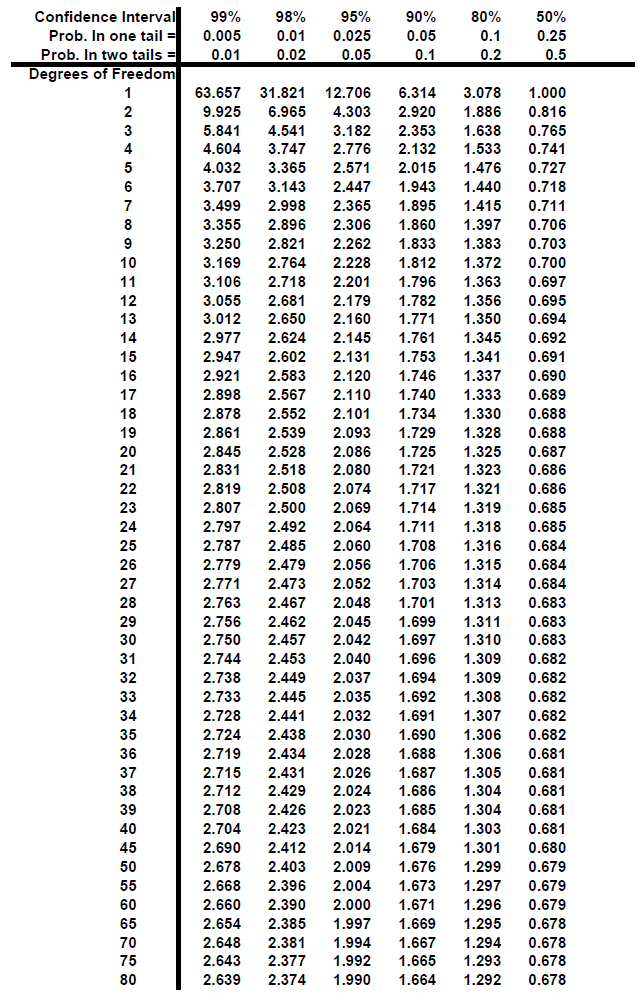
\includegraphics[width=1\textwidth]{pics/tdist-1.png}
\end{center}
\clearpage


\begin{center}
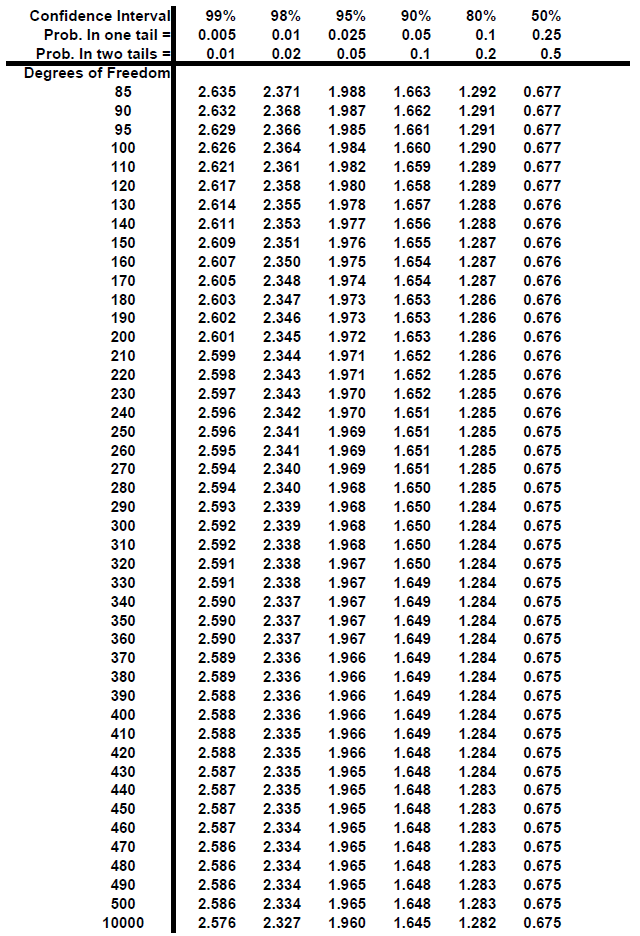
\includegraphics[width=1\textwidth]{pics/tdist-2.png}
\end{center}
\clearpage
   
\addChapter{Hasil Ujicoba}
\chapter*{Hasil Ujicoba}

\end{appendix}

\end{document}